% Generated from Markdown by scripts/build_revision_v8_publication.py; do not edit numeric content manually.
% Options for packages loaded elsewhere
\PassOptionsToPackage{unicode}{hyperref}
\PassOptionsToPackage{hyphens}{url}
\PassOptionsToPackage{dvipsnames,svgnames,x11names}{xcolor}
\documentclass[
  10pt,
]{ctexart}
\usepackage{xcolor}
\usepackage[margin=18mm]{geometry}
\usepackage{amsmath,amssymb}
\setcounter{secnumdepth}{-\maxdimen} % remove section numbering
\usepackage{iftex}
\ifPDFTeX
  \usepackage[T1]{fontenc}
  \usepackage[utf8]{inputenc}
  \usepackage{textcomp} % provide euro and other symbols
\else % if luatex or xetex
  \usepackage{unicode-math} % this also loads fontspec
  \defaultfontfeatures{Scale=MatchLowercase}
  \defaultfontfeatures[\rmfamily]{Ligatures=TeX,Scale=1}
\fi
\usepackage{lmodern}
\ifPDFTeX\else
  % xetex/luatex font selection
\fi
% Use upquote if available, for straight quotes in verbatim environments
\IfFileExists{upquote.sty}{\usepackage{upquote}}{}
\IfFileExists{microtype.sty}{% use microtype if available
  \usepackage[]{microtype}
  \UseMicrotypeSet[protrusion]{basicmath} % disable protrusion for tt fonts
}{}
\makeatletter
\@ifundefined{KOMAClassName}{% if non-KOMA class
  \IfFileExists{parskip.sty}{%
    \usepackage{parskip}
  }{% else
    \setlength{\parindent}{0pt}
    \setlength{\parskip}{6pt plus 2pt minus 1pt}}
}{% if KOMA class
  \KOMAoptions{parskip=half}}
\makeatother
\usepackage{longtable,booktabs,array}
\newcounter{none} % for unnumbered tables
\usepackage{calc} % for calculating minipage widths
% Correct order of tables after \paragraph or \subparagraph
\usepackage{etoolbox}
\makeatletter
\patchcmd\longtable{\par}{\if@noskipsec\mbox{}\fi\par}{}{}
\makeatother
% Allow footnotes in longtable head/foot
\IfFileExists{footnotehyper.sty}{\usepackage{footnotehyper}}{\usepackage{footnote}}
\makesavenoteenv{longtable}
\usepackage{graphicx}
\makeatletter
\newsavebox\pandoc@box
\newcommand*\pandocbounded[1]{% scales image to fit in text height/width
  \sbox\pandoc@box{#1}%
  \Gscale@div\@tempa{\textheight}{\dimexpr\ht\pandoc@box+\dp\pandoc@box\relax}%
  \Gscale@div\@tempb{\linewidth}{\wd\pandoc@box}%
  \ifdim\@tempb\p@<\@tempa\p@\let\@tempa\@tempb\fi% select the smaller of both
  \ifdim\@tempa\p@<\p@\scalebox{\@tempa}{\usebox\pandoc@box}%
  \else\usebox{\pandoc@box}%
  \fi%
}
% Set default figure placement to htbp
\def\fps@figure{htbp}
\makeatother
% definitions for citeproc citations
\NewDocumentCommand\citeproctext{}{}
\NewDocumentCommand\citeproc{mm}{%
  \begingroup\def\citeproctext{#2}\cite{#1}\endgroup}
\makeatletter
 % allow citations to break across lines
 \let\@cite@ofmt\@firstofone
 % avoid brackets around text for \cite:
 \def\@biblabel#1{}
 \def\@cite#1#2{{#1\if@tempswa , #2\fi}}
\makeatother
\newlength{\cslhangindent}
\setlength{\cslhangindent}{1.5em}
\newlength{\csllabelwidth}
\setlength{\csllabelwidth}{3em}
\newenvironment{CSLReferences}[2] % #1 hanging-indent, #2 entry-spacing
 {\begin{list}{}{%
  \setlength{\itemindent}{0pt}
  \setlength{\leftmargin}{0pt}
  \setlength{\parsep}{0pt}
  % turn on hanging indent if param 1 is 1
  \ifodd #1
   \setlength{\leftmargin}{\cslhangindent}
   \setlength{\itemindent}{-1\cslhangindent}
  \fi
  % set entry spacing
  \setlength{\itemsep}{#2\baselineskip}}}
 {\end{list}}
\usepackage{calc}
\newcommand{\CSLBlock}[1]{\hfill\break\parbox[t]{\linewidth}{\strut\ignorespaces#1\strut}}
\newcommand{\CSLLeftMargin}[1]{\parbox[t]{\csllabelwidth}{\strut#1\strut}}
\newcommand{\CSLRightInline}[1]{\parbox[t]{\linewidth - \csllabelwidth}{\strut#1\strut}}
\newcommand{\CSLIndent}[1]{\hspace{\cslhangindent}#1}
\setlength{\emergencystretch}{3em} % prevent overfull lines
\providecommand{\tightlist}{%
  \setlength{\itemsep}{0pt}\setlength{\parskip}{0pt}}
\usepackage{bookmark}
\IfFileExists{xurl.sty}{\usepackage{xurl}}{} % add URL line breaks if available
\urlstyle{same}
\hypersetup{
  pdftitle={面向视觉 Transformer 内部目标的双索引局部 Jacobian 扫描与结构审计},
  colorlinks=true,
  linkcolor={Maroon},
  filecolor={Maroon},
  citecolor={Blue},
  urlcolor={Blue},
  pdfcreator={LaTeX via pandoc}}

\title{面向视觉 Transformer 内部目标的双索引局部 Jacobian
扫描与结构审计}
\author{}
\date{}

\begin{document}
\hypersetup{pdfauthor={},pdfsubject={},pdfkeywords={}}
\maketitle

\section{摘要}\label{ux6458ux8981}

当神经网络扫描器（Neural Network
Scanner，NNS）使用当前点的精确局部导数且不作额外重分配时，标量 learning
image 等于同目标的 Gradient × Input；本文将归一化输入坐标下的这一量称为
Endpoint。普通 Gradient × Input
保留输入坐标，却不显式区分同一中间表示被哪个后续算子及其哪个输入槽使用。为此，本文面向固定
Vision
Transformer（ViT）计算图，提出同时索引输入坐标与具体张量使用位置的局部微分表示。该表示将标量目标分解为
attention head、Q/K/V、routing/value 与 residual identity/branch
等结构分项，并分别在分支切面和全局切面上重构对应的局部微分。面向实际 ViT
拓扑的图结构认证、数值闭合、独立解析实现和故障注入共同验证了分解的完整性与实现正确性。

在两个固定模型检查点上，双索引图揭示了清晰的层深空间组织。单元目标的输入依赖总体向更广空间扩展，K/V
分项熵随深度下降，attention 与 MLP residual
呈现可区分的空间重组和尺度轨迹。低总质量分层与截尾分析均保持空间扩展方向，三种输入坐标量保留多数主要趋势；独立图像队列和四个公开模型检查点进一步复现了单元扩展、路由分配与残差轨迹。由此，双索引表示能够在统一输入坐标中比较不同内部模块的空间依赖，并定位总图或单一成分标量无法恢复的结构差异。

本文由此建立了面向 ViT 内部目标的 Endpoint
扫描框架：以统一输入坐标呈现标量目标的局部依赖，以具体张量 use 保留
attention、MLP 与 residual
的结构身份，并用合法切面将分项重构到同一目标。该框架把内部目标可视化推进为可分解、可闭合验证和可跨模块比较的结构分析。有限替换实验进一步界定了它的使用方式：Endpoint
适合描述当前状态的结构化局部依赖；涉及特定参考状态的干预排序时，可在同一分析框架中加入实际位移信息。

关键词：视觉 Transformer；Neural Network Scanner；Gradient × Input；局部
Jacobian；结构审计

\section{1. 引言}\label{ux5f15ux8a00}

视觉 Transformer（ViT）将图像划分为 patch
tokens，随后通过自注意力和前馈网络逐层建立表示（Dosovitskiy et al.,
2021）。这一结构能够处理不同位置间的关系，也使内部计算的解释更加复杂：token-channel
单元描述特定位置的响应，attention head
在多个位置间传递信息，残差连接又将输入与分支输出叠加。要理解这些对象之间的联系，需要一种能够保留输入空间位置、并适用于不同内部对象的表示。

现有可视化通常展示特征图、注意力权重或类别相关区域。这些视图各有用途，但其空间分辨率、目标和传播规则不同。前向特征图说明一个通道在
token 网格上的响应，attention 权重说明 token
间的分配关系；它们与某个内部标量关于原始图像的依赖并不是同一个对象。将内部目标映射回统一输入坐标，可以为跨模块比较提供共同的观察基础。本文所称``路径图''是指定
tensor use 的局部微分分项，不是唯一因果路径。

Neural Network Scanner（NNS）为神经元关联一张保留输入位置的 learning
image（Dou et al.,
2023）。原方法的逐层尺度传播在使用实际局部导数时可以写成 Jacobian
链式法则；对标量目标，其终点学习图像就是 Input ×
Gradient。这个恒等式确定了本文的局部测量原语。本文进一步保留两个自由索引。输入坐标
\(i\) 记录局部依赖出现在哪里，实际 consumer-use edge \(e\)
记录该项经过哪一次具体使用。总图对 \(e\) 求和，无法区分 Q/K/V 或
identity/branch 的空间分配；edge scalar 对 \(i\)
求和，无法计算分项熵、空间 TV 或空间抵消。目标 registry 固定条件
\(s\)，结构合法切面把分项绑定回同一总局部微分。双索引图组由此回答同一局部微分如何在指定
use 与输入位置之间重新分配，并检查声明的切面合同。

\refstepcounter{figure}\label{fig:zh-manuscript-001}
\pandocbounded{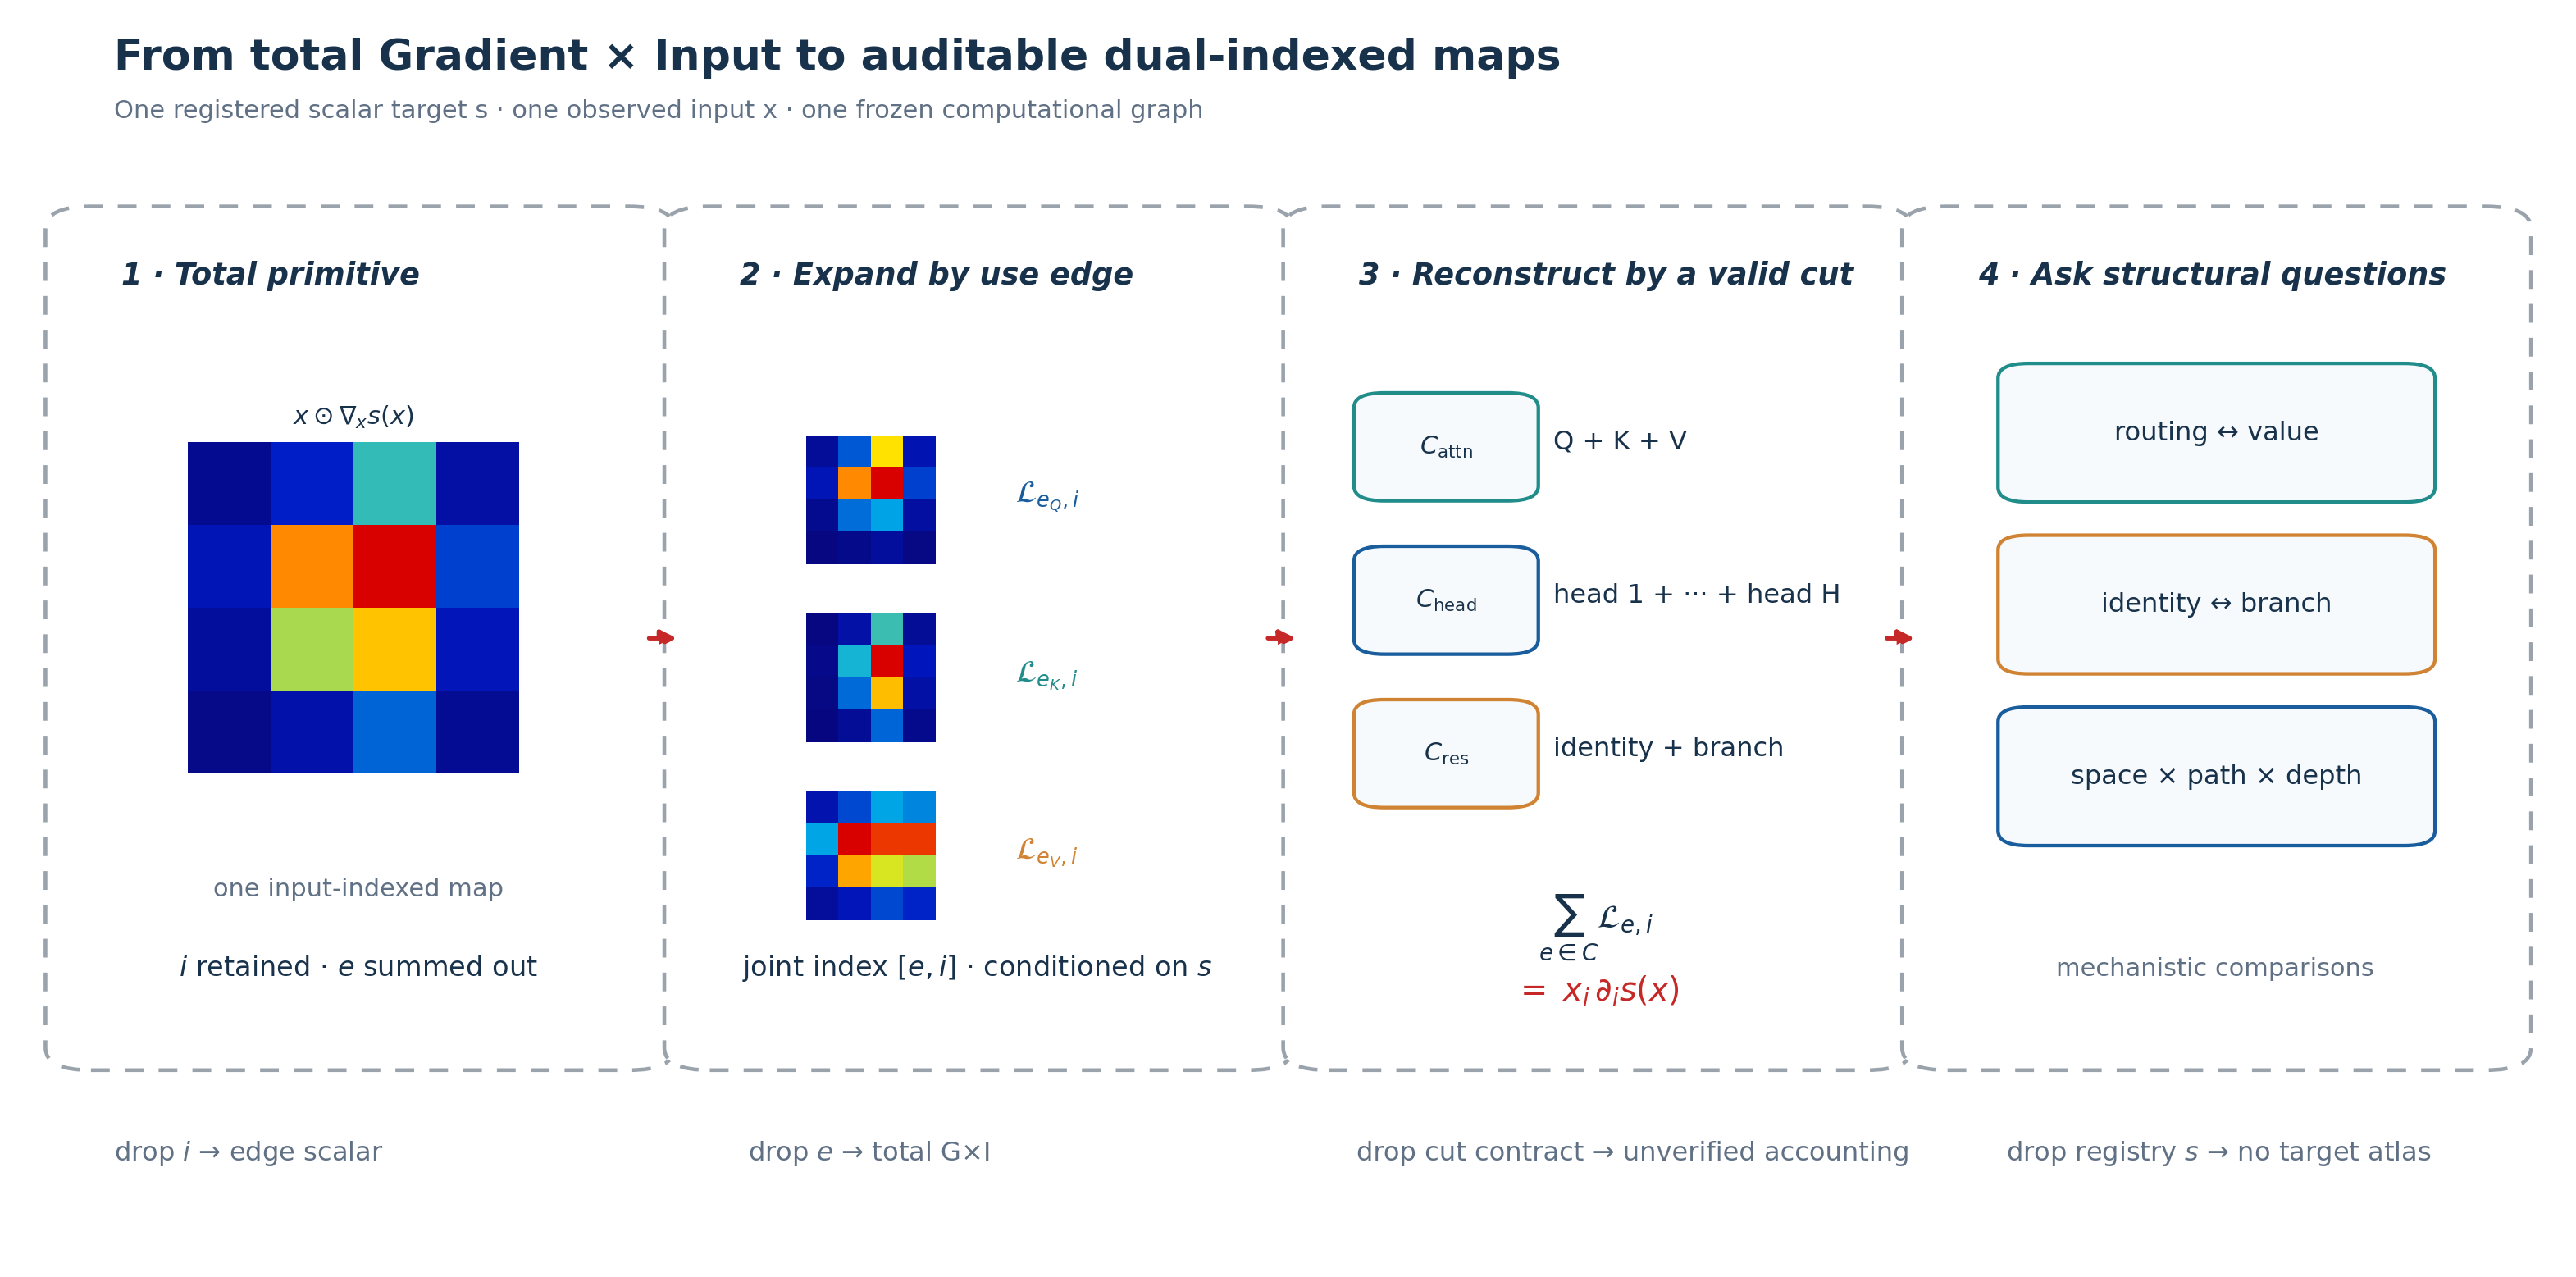
\includegraphics[keepaspectratio,alt={Figure 1}]{../figures/png/fig_01_concept_overview.png}}

\textbf{Figure 1.} 左侧为固定目标和输入点的 Total Endpoint。中间保留原生
use 身份与输入坐标，并将 attention
分支内部的微分分组单独定义。右侧分别比较空间分布与规定有限替换效应。全局闭合须包含
residual bypass；分支分组只重构 attention branch contribution。

本文的总体问题是：如何在 NNS 框架下，将 ViT
内部目标对输入的局部依赖表示为可计算、可分解和可验证的结构路径图，并评价其层深分布轨迹及在规定有限替换任务中的排序能力？具体研究四个问题：

\begin{enumerate}
\def\labelenumi{\arabic{enumi}.}
\tightlist
\item
  \textbf{数学对象：NNS 学习图像表示什么？} 明确逐层尺度传播、Jacobian
  链式法则与 Input × Gradient 的关系，以及非齐次项、固定 token
  和输入坐标原点带来的限制。
\item
  \textbf{结构推广：如何将 NNS 用于 ViT 计算图？}
  定义内部标量目标、真实计算边、合法计算切面及 attention、multi-head 和
  residual 的可加局部微分路径。
\item
  \textbf{空间分布：结构分项如何随深度变化？} 在两个固定预训练
  checkpoint 的冻结抽样目标上分析空间扩展、routing/value 与
  identity/branch
  的层深分布轨迹，并比较训练参数状态和随机参数状态以及目标与抽样控制。
\item
  \textbf{有限替换效用：局部微分分数能否排序规定的有限替换效应？} 比较
  clean-state 路径分数、activation × gradient 和包含实际 activation
  displacement 的一阶 Taylor 分数。
\end{enumerate}

方法贡献有两点。第一，给出目标条件化的双索引局部微分表示，明确全局切面与分支分组各自的闭合对象。第二，建立面向
ViT use
身份、遗漏和重复的结构审计，用架构图认证与独立解析参考逐项检查组件图。经验分析另行回答固定
checkpoint
上的空间分布与有限替换排序问题。总图描述整体空间扩展，成对分项图描述
attention 与 residual 的空间差异；路径图未提高 head
有限替换排序，结构分辨率不等于干预预测能力。

下文先界定相关方法与本文定位，再给出 NNS 的一般 Jacobian 表示和 ViT
结构分解。实验按等价性与闭合、层深分布轨迹、结构路径和有限干预组织，最后讨论证据范围。

\section{2. 相关工作}\label{ux76f8ux5173ux5de5ux4f5c}

\subsection{2.1 NNS
与学习图像}\label{nns-ux4e0eux5b66ux4e60ux56feux50cf}

神经元可视化通过输入模式或实际样本分析内部响应。NNS
将单个神经元的计算组织为输入坐标 learning image，并用
activation-weighted aggregation 表示卷积通道（Dou et al.,
2023）。这种组织方式使不同原生空间结构的内部对象能够映射到同一图像坐标。本文保留``学习图像''这一历史术语；在数学推导中称其为``局部输入依赖图''，以强调它描述当前输入点的一阶响应。

\subsection{2.2 局部梯度、路径积分、FullGrad
与隐藏单元归因}\label{ux5c40ux90e8ux68afux5ea6ux8defux5f84ux79efux5206fullgrad-ux4e0eux9690ux85cfux5355ux5143ux5f52ux56e0}

Gradient × Input 是观测点上的输入加权梯度（Shrikumar et al.,
2017）；Integrated Gradients 沿 reference
到输入的路径平均梯度并满足相应完整性公理（Sundararajan et al.,
2017），conductance 将该路径归因扩展到隐藏单元（Dhamdhere et al.,
2018）。FullGrad 将输入梯度项与各层 bias-gradient
项共同组成完整表示，再聚合为显著图（Srinivas and Fleuret, 2019）。本文的
Endpoint 使用当前点的真实 Jacobian，不进行路径积分，也不把 bias
项加入输入图。因此 conductance 的路径完整性、FullGrad
的函数值完整表示和本文合法切面的局部微分闭合是三个不同对象。

DAVE 将 ViT 输入梯度分为直接 effective input-output transformation 与
local-variation 项，再跨输入分布聚合保留项（Wróbel et al., 2026）。它是
ViT 梯度结构分解和空间归因的直接先例，但不保留按内部 consumer use
索引的一组输入坐标图。

\subsection{2.3 Transformer token contribution 与 relevance
传播}\label{transformer-token-contribution-ux4e0e-relevance-ux4f20ux64ad}

GlobEnc 把 encoder block 的 attention、residual 与 normalization
纳入逐层 token attribution，并跨层聚合（Modarressi et al., 2022）。ALTI
分解包含 residual 与 LayerNorm 的整个 attention block 的 token
interaction，再用 rollout 聚合；其发表版本未纳入 classifier（Ferrando et
al., 2022）。DecompX 传播 token representation
分量，覆盖非线性前馈层和分类头，并按其 bias 分配规则重组 representation
与 logit（Modarressi et al., 2023）。

AttnLRP 为 softmax、双线性 attention、normalization 与 latent
attribution 定义 relevance rule（Achtibat et al., 2024）。LibraGrad 在
FullGrad-completeness 目标下剪枝和缩放反向路径，用于 ViT
attribution（Mehri et al., 2025）。HiLRP 将多类 ViT attention
和分辨率变化模块归约为四类守恒 primitive，并以机器精度验证
conservation；GradSkip 则显式在 attention 与 residual 路径之间动态分配
relevance（Nishankar et al., 2026; Buratti et al., 2026）。Unpack
不依赖梯度即可生成 component interaction、带 K/Q/V composition label
的命名端到端路径和 token attribution（Chen et al.,
2026）。这些工作已经为 Transformer 组件传播、Q/K/V 分析、skip-aware
分配和精确守恒提供直接先例。本文比较的差异因此是保留的索引与闭合对象：不修改模型的真实局部导数、具体
consumer use
的输入坐标分项，以及这些分项在合法切面上对同一局部微分的加和重构。

\subsection{2.4 Activation patching 与 edge
attribution}\label{activation-patching-ux4e0e-edge-attribution}

Activation patching 以 clean/corrupted reference
替换真实内部变量并测量有限输出变化；结果依赖
corruption、替换位置和评价指标（Zhang and Nanda, 2023）。Attribution
patching 以 activation displacement 与局部梯度的内积近似单个组件的
patching effect；Edge attribution patching 将这一近似用于计算图边（Syed
et al., 2024）。AtP* 进一步处理 attention saturation
与抵消造成的近似误差（Kramár et al., 2024）。这些方法直接评价或近似
reference-specified finite effect。本文分别报告 clean-only
路径图、reference-aware Taylor
量和真实替换效应，不用结构闭合代替有限干预效用。

边分析和内部干预也已经进入视觉领域。Vi-CD 通过 activation patching 在
ViT 与 OpenCLIP 中发现并验证稀疏 residual-stream edge circuits（Żukowska
et al., 2026）；CAAP 将源图像 activation 插入中性上下文以构造 ViT patch
attribution（Izadi et al., 2026）。真实边和 ViT activation patching
均为已有先例。

\subsection{2.5
视觉归因与本文定位}\label{ux89c6ux89c9ux5f52ux56e0ux4e0eux672cux6587ux5b9aux4f4d}

Grad-CAM 通过梯度加权特征图获得类别相关定位（Selvaraju et al.,
2017），attention rollout 组合跨层 attention flow（Abnar and Zuidema,
2020），Chefer et al.（2021）则为 Transformer 设计 relevance
传播。它们与 Gradient × Input、token decomposition、LRP
和有限替换面向不同解释对象。Table 1
集中比较五个最近邻方法族；完整方法矩阵移至补充材料。``未报告''只指核验版本没有给出相应对象。本轮在线核验日期为
2026 年 9 月 23 日（PRC）；DAVE、Vi-CD、CAAP、HiLRP、GradSkip 与 Unpack
均按相应 arXiv 版本标为预印本。

\refstepcounter{table}\label{tab:zh-manuscript-001}
\textbf{Table 1. 与五个最近邻方法族的对象级比较}

{\def\LTcaptype{none} % do not increment counter
\begingroup\scriptsize
\setlength{\tabcolsep}{2pt}
\begin{longtable}[]{@{}
  >{\raggedright\arraybackslash}p{(\linewidth - 8\tabcolsep) * \real{0.2000}}
  >{\raggedright\arraybackslash}p{(\linewidth - 8\tabcolsep) * \real{0.2000}}
  >{\raggedright\arraybackslash}p{(\linewidth - 8\tabcolsep) * \real{0.2000}}
  >{\raggedright\arraybackslash}p{(\linewidth - 8\tabcolsep) * \real{0.2000}}
  >{\raggedright\arraybackslash}p{(\linewidth - 8\tabcolsep) * \real{0.2000}}@{}}
\toprule\noalign{}
\begin{minipage}[b]{\linewidth}\raggedright
Method family
\end{minipage} & \begin{minipage}[b]{\linewidth}\raggedright
Primary object
\end{minipage} & \begin{minipage}[b]{\linewidth}\raggedright
Index retained
\end{minipage} & \begin{minipage}[b]{\linewidth}\raggedright
Reconstruction target
\end{minipage} & \begin{minipage}[b]{\linewidth}\raggedright
Empirical role
\end{minipage} \\
\midrule\noalign{}
\endhead
\bottomrule\noalign{}
\endlastfoot
Conductance & Reference-to-input path attribution through hidden units &
Hidden unit and input & Output difference across a layer & Hidden-unit
attribution \\
DecompX / LRP & Token representation or relevance components &
Token/operator, method-dependent & Representation, logit or conserved
relevance & Token attribution and localization \\
EAP / AtP* / Vi-CD & Reference-specific component or edge effects &
Component/edge & Patching effect or circuit fidelity & Circuit
localization and intervention \\
DAVE & Distribution-aware ViT input-gradient decomposition & Input
position and gradient term & Effective input--output map & ViT spatial
attribution \\
Unpack & Component interactions and named K/Q/V paths & Component/path
and token & Method-specific credit decomposition & Composition and token
credit \\
NNS--ViT & Current-point local differential by concrete use and input
position & Consumer use \(e\) and input coordinate \(i\) & Branch
contribution or same-target total differential, according to the
declared cut & Structural audit and spatial comparison \\
\end{longtable}
\endgroup
}

Conductance 用输出差定义路径完整性，DecompX/LRP 重组表示或
relevance，EAP/Vi-CD 面向 reference-specific 边效应，DAVE 分解 ViT
输入梯度，Unpack 保留命名组件路径。本文的技术差异是当前点微分在具体 use
与输入位置上的联合表示及对声明切面合同的实现一致性检查。基础 Gradient ×
Input、组件分解和 activation patching 均为已有方法。

\section{3. NNS 的 Jacobian
解释}\label{nns-ux7684-jacobian-ux89e3ux91ca}

\subsection{3.1 NNS
的一般计算图表示}\label{nns-ux7684ux4e00ux822cux8ba1ux7b97ux56feux8868ux793a}

设网络为有向无环计算图 \(G=(V,E)\)，输入为 \(x\)，目标为标量
\(s(x)\)。一个神经元输出标量值，学习图像则保留该标量所依赖的输入坐标。Figure
1 先区分总 Gradient × Input 与本文的双索引展开；坐标初始化和原始 NNS
逐层传播示意保留在补充图件。本文将最终标量图记为 \(E_s(x)\)，并称为 NNS
局部输入图。

设图像输入为列向量 \(x\in\mathbb R^d\)，标量梯度
\(\nabla_xs\in\mathbb R^d\) 也按列向量记。对
\(u(x)\in\mathbb R^m\)，learning-image 矩阵为
\(\mathcal L(u;x)\in\mathbb R^{m\times d}\)。初始化与传播规则为

\begin{equation}\label{eq:zh-manuscript-001}
\mathcal L(x;x)=\operatorname{diag}(x),\qquad
\mathcal L(v;x)=\sum_aJ_{f,u_a}(x)\mathcal L(u_a;x),\quad v=f(u_1,\ldots,u_r).
\end{equation}

\textbf{命题 1（标量目标等价性）。} 若所有局部 Jacobian
在同一当前前向状态求值，且传播中不引入归一化、截断或相关性重分配，则

\begin{equation}\label{eq:zh-manuscript-002}
\mathcal L(u;x)=J_{u,x}(x)\operatorname{diag}(x),\qquad
\mathcal L(s;x)=\nabla_xs(x)^\top\operatorname{diag}(x),\qquad
E_s(x)=\mathcal L(s;x)^\top=\operatorname{diag}(x)\nabla_xs(x).
\end{equation}

\textbf{证明。} 输入处
\(J_{x,x}=I\)。按计算图拓扑顺序递推，将各前驱的表达式代入传播规则，再使用多输入链式法则，即得到每个节点的结论。对标量节点转置得到列向量
Endpoint。在线性、卷积和当前 ReLU gate 下，该规则恢复原始 NNS
系数；MaxPool 使用当前前向 winner。ReLU 零点和 MaxPool
并列遵循框架的固定导数选择，光滑区域内使用通常导数。

Endpoint 表示当前点上目标关于各输入坐标缩放方向的局部一阶依赖：对
\(x_i\mapsto(1+\epsilon)x_i\)，其一阶响应为 \(\epsilon E_{s,i}\)。一般有

\begin{equation}\label{eq:zh-manuscript-003}
\sum_iE_{s,i}=x^\top\nabla_xs(x)\ne s(x).
\end{equation}

一阶齐次函数在可微点可由 Euler 定理得到等号；含 bias、固定
token、位置编码、LayerNorm、softmax 和 GELU 的一般 ViT
不满足这一条件。Endpoint 重构局部输入 Jacobian
分解，不能作为目标全部来源或函数值的完整分解。CLS token、位置编码和
patch/LN/QKV/MLP/classifier 的偏置没有独立图像坐标项，但会改变当前函数和
Jacobian。

若 \(x=(r-\mu)/\sigma\)，则

\begin{equation}\label{eq:zh-manuscript-004}
x_i\frac{\partial s}{\partial x_i}=(r_i-\mu_i)\frac{\partial s}{\partial r_i}.
\end{equation}

因此 Endpoint 不需要外部选择的 intervention
reference，但依赖模型输入坐标及 normalization origin。

\section{4. ViT
内部目标的双索引局部微分}\label{vit-ux5185ux90e8ux76eeux6807ux7684ux53ccux7d22ux5f15ux5c40ux90e8ux5faeux5206}

\subsection{4.1 Target registry
与双索引对象}\label{target-registry-ux4e0eux53ccux7d22ux5f15ux5bf9ux8c61}

本文将机器合同分成三类。标量目标 registry 固定读出
\(s\)、图中位置和聚合规则；局部微分分解 registry 固定 native
use、解析分组、cut 与重构对象；有限替换 registry
固定可干预变量、reference 和
effect。三类对象不能互换：Q/K/V-induced、routing/value 和 residual
identity/branch 是局部微分分项，不计入标量目标数；attention
probability、value projection、head output 与 residual branch activation
是干预变量，也不因可替换而成为标量读出。对于通道 \(c\) 的 patch
activations，聚合目标可定义为

\begin{equation}\label{eq:zh-manuscript-005}
s_{\mathrm{energy}}=\frac12\sum_{t=1}^{196}h_{t,c}^2,\qquad
\nabla_xs_{\mathrm{energy}}=\sum_th_{t,c}\nabla_xh_{t,c},\qquad
E_{\mathrm{energy}}=\sum_th_{t,c}E_{h_{t,c}}.
\end{equation}

这给出原始 NNS activation-weighted filter aggregation 的 Jacobian
形式；energy 是聚合标量而非单个神经元。每图标量目标包括 192 个
post-block token-channel、48 个 post-block patch sum、48 个 post-block
patch energy、ViT-B/DeiT-S 各 144/72 个 attention-head coordinate、18 个
module patch aggregate、4 个 patch-embedding aggregate、1 个 final-CLS
coordinate 和 2 个类别 logits，合计
457/385。它们是冻结的结构锚点，不是对全部神经元的穷举或统计代表样本。跨模型同编号
channel 不视为同语义单元。

Registry
只声明目标位置和读出语义，不会使某个目标自动获得全部切面。对现有 457/385
个目标的 module、location 与 kind 字段审计得到以下适用规则。

{\def\LTcaptype{none} % do not increment counter
\begingroup\scriptsize
\setlength{\tabcolsep}{2pt}
\begin{longtable}[]{@{}
  >{\raggedright\arraybackslash}p{(\linewidth - 6\tabcolsep) * \real{0.2500}}
  >{\raggedright\arraybackslash}p{(\linewidth - 6\tabcolsep) * \real{0.2500}}
  >{\raggedright\arraybackslash}p{(\linewidth - 6\tabcolsep) * \real{0.2500}}
  >{\raggedright\arraybackslash}p{(\linewidth - 6\tabcolsep) * \real{0.2500}}@{}}
\toprule\noalign{}
\begin{minipage}[b]{\linewidth}\raggedright
目标类型或位置
\end{minipage} & \begin{minipage}[b]{\linewidth}\raggedright
可用的全局切面
\end{minipage} & \begin{minipage}[b]{\linewidth}\raggedright
可用的分支分组
\end{minipage} & \begin{minipage}[b]{\linewidth}\raggedright
不适用条件
\end{minipage} \\
\midrule\noalign{}
\endhead
\bottomrule\noalign{}
\endlastfoot
最终类别 logit & 指定 residual 的 identity 加完整 branch partition & 该
residual 上游的 attention branch & 无 \\
residual 输出之后的内部标量 & 位于目标上游且截断全部输入路径的 residual
cut & 对应上游 branch & 切面位于目标下游 \\
residual 之前或 branch 内部目标 & 仅由目标祖先子图决定的 cut &
仅在目标位于该 branch 下游时 & 不得套用后续 residual 全局等式 \\
energy 或 patch-sum 聚合目标 & 由实际 module/location 读出位置决定 &
由实际祖先关系决定 & 不因进入 registry 自动获得全部切面 \\
\end{longtable}
\endgroup
}

该适用表另由冻结架构图逐项认证。对两个标准 12-block pre-LN ViT，显式展开
patch embedding、Q/K/V、各 head use、attention projection、两次 residual
addition、MLP、final norm 和 classifier；随后对全部 842 个标量目标、12
层和 8 类 cut 做图遍历，共 80,832 个 target--cut 配对。完整 target cut
要求其全部声明边位于目标祖先子图，且每条输入到目标路径恰好穿过一次；branch
partition 则只认证对 attention branch contribution 的完整截断，并要求该
branch 位于目标上游。结果将 26,094 个配对认证为完整 target cut、15,660
个认证为合法 branch-only partition，其余 39,078
个明确记为目标上游或重构对象不适用。该认证针对 registry 绑定的标准
unfused pre-LN 架构，不覆盖带额外分支或不同算子融合的实现。

令实际使用边

\begin{equation}\label{eq:zh-manuscript-006}
e=(p_e,c_e,q_e,\nu_e),
\end{equation}

由 producer \(p_e\)、consumer \(c_e\)、consumer input slot \(q_e\) 与
invocation \(\nu_e\) 联合确定。\(z_e(x)\) 是 producer 输出进入该
consumer use 时的张量。\(\bar z_e^{(s)}\) 是在该 input slot
处、尚未与同一 producer 的其他 fan-out uses 合并的 target
cotangent。本文定义

\begin{equation}\label{eq:zh-manuscript-007}
\boxed{
\mathcal L_{e,i}(s;x)
=x_i\left[J_{z_e,x}(x)^{\mathsf T}\bar z_e^{(s)}\right]_i.
}
\end{equation}

\(i\) 与 \(e\) 是自由索引，\(s\) 是 registry
选定的目标条件。Jacobian、cotangent 和 \(z_e\) 均在同一观测输入 \(x\)
和同一前向状态求值。固定 \(e\) 得到一张保留输入位置的图；固定 \(i\)
可比较同一输入坐标经不同实际使用边的局部项；在全局切面上对 \(e\)
求和则回到总量。该表示同时保留 use 与输入位置。Total Endpoint 仍为已有的
Gradient × Input。

同一 producer tensor 可同时进入多个 consumer，也可进入同一 consumer
的不同 slot，或在重复调用中被多次使用。此时 \(J_{z_e,x}\)
可以共享上游数值，但 \(\bar z_e^{(s)}\) 对应不同下游 use。按 tensor name
合并这些 cotangent 会提前丢失路径身份，因此 edge identity 必须包含
consumer、slot 与 invocation。Figure 2 将这一合同与 ViT 切面实例并列。

\refstepcounter{figure}\label{fig:zh-manuscript-002}
\pandocbounded{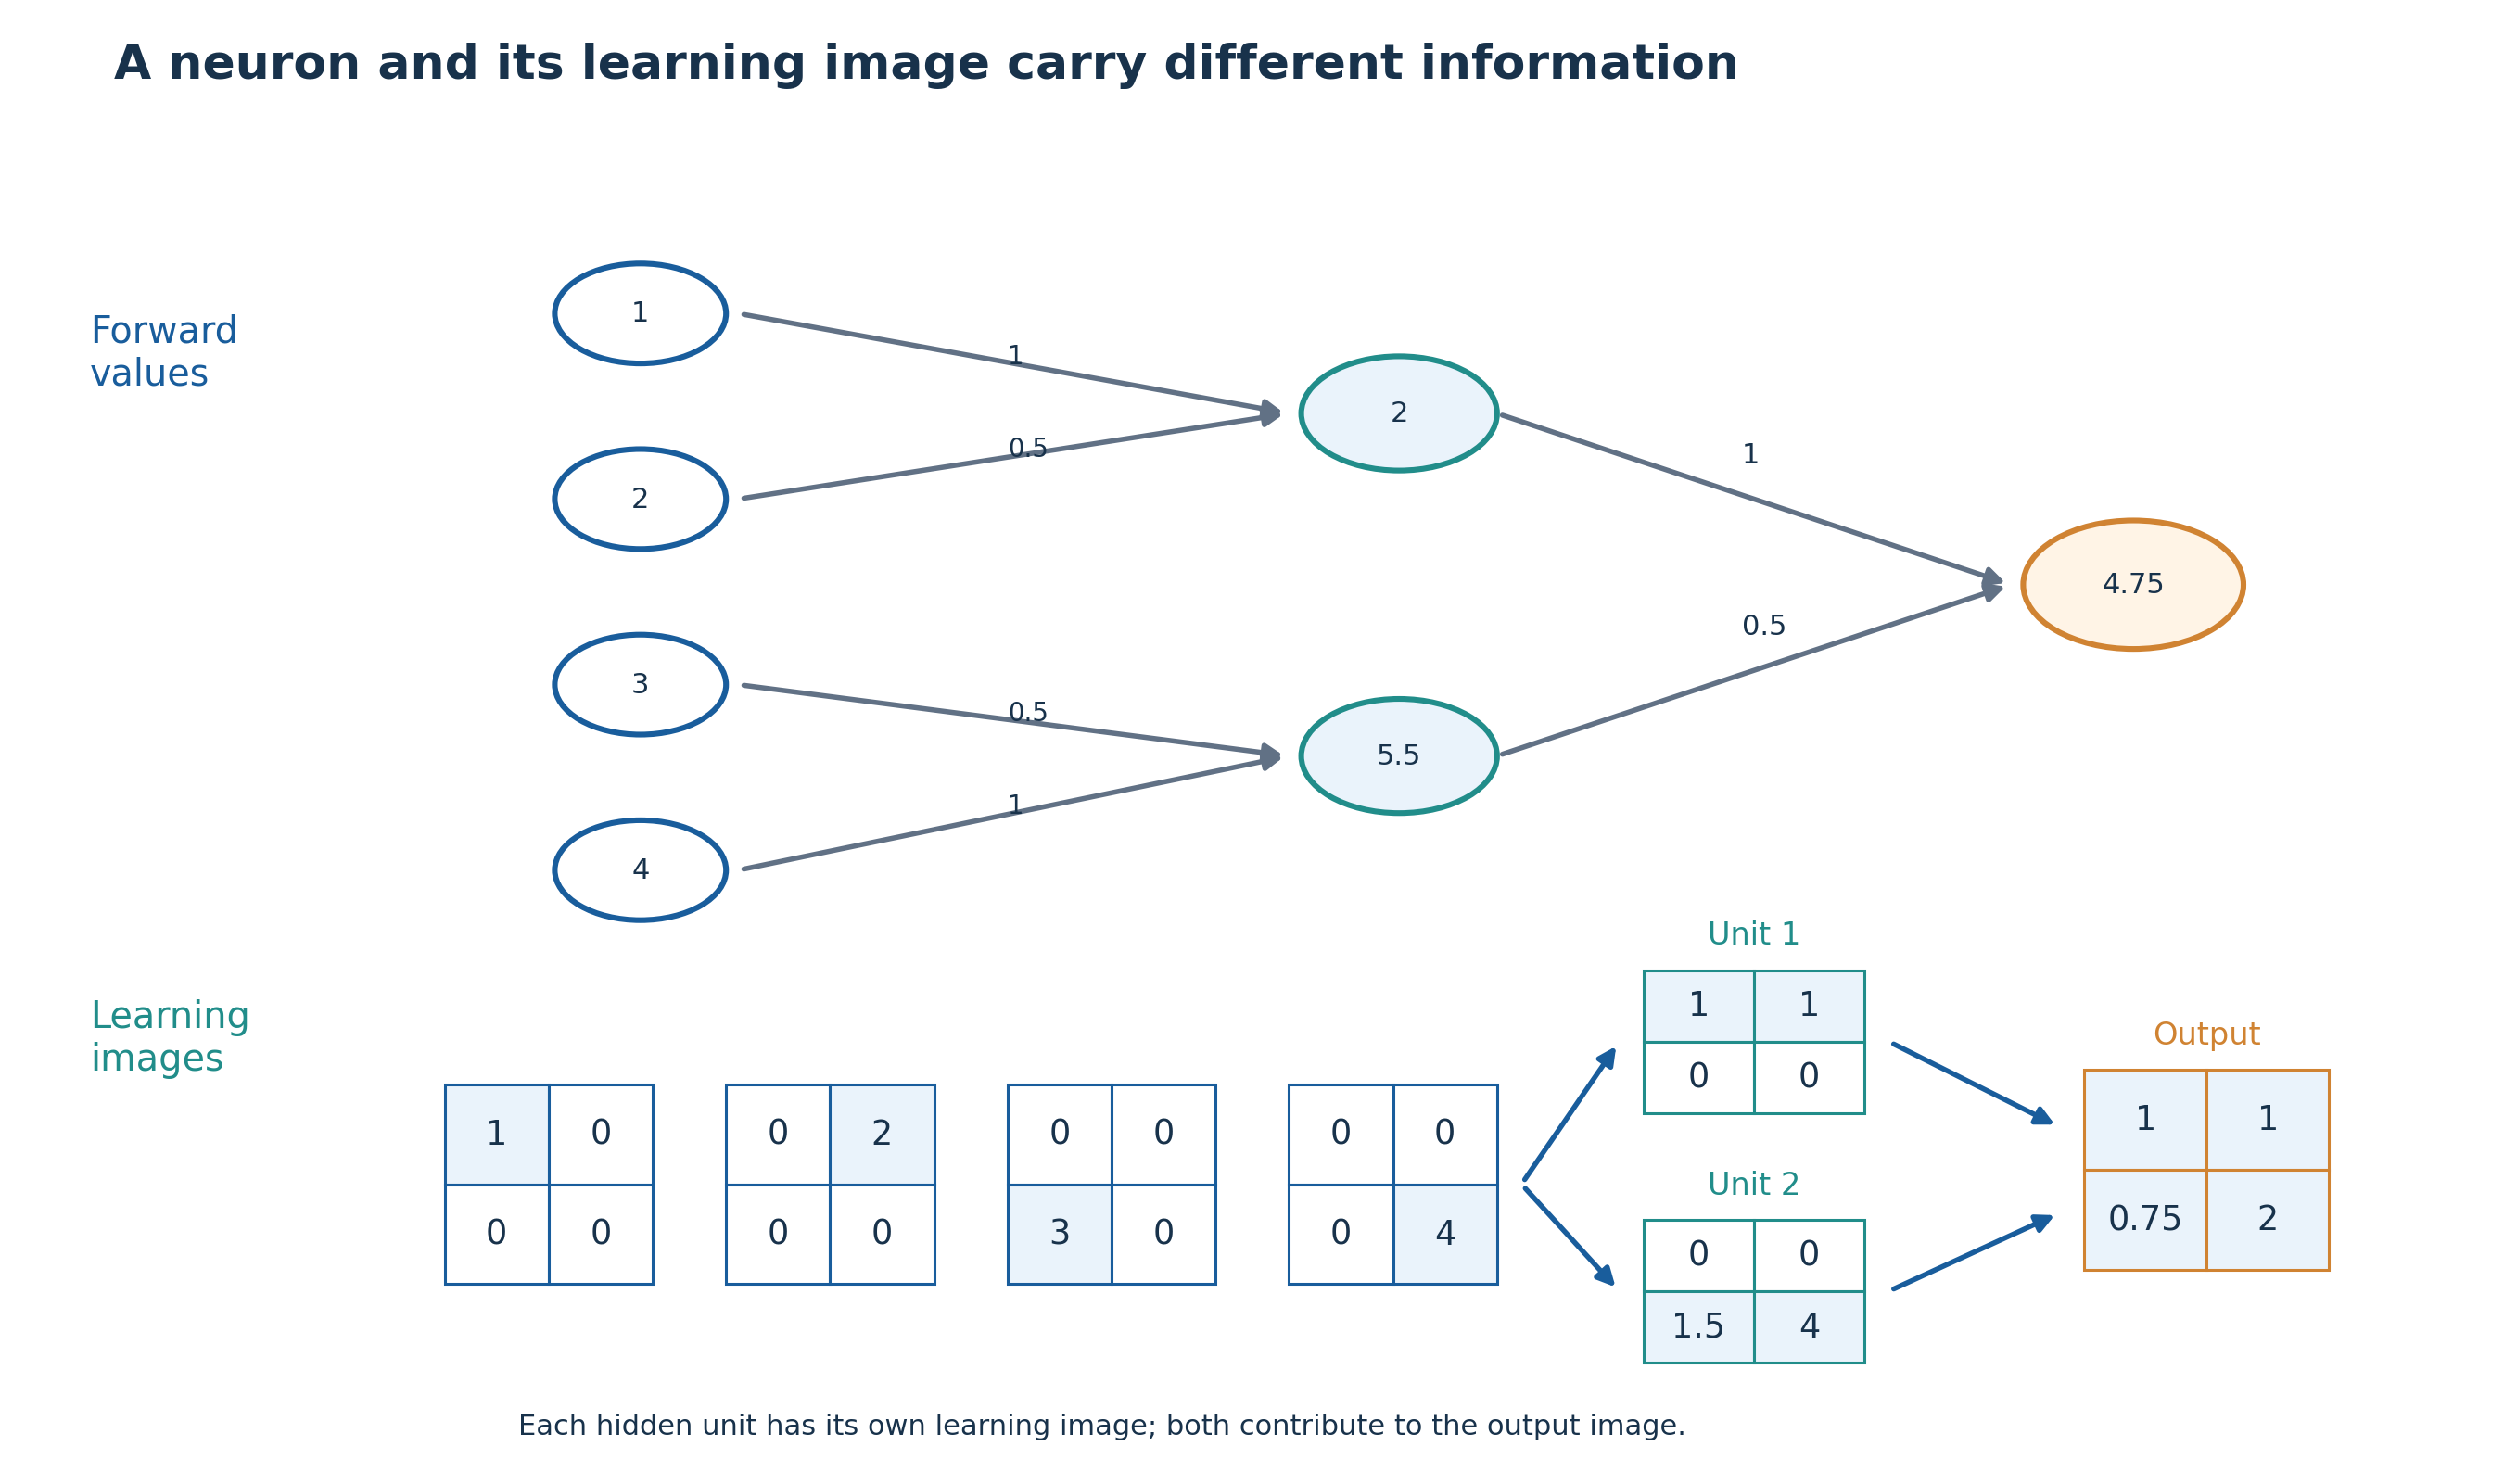
\includegraphics[keepaspectratio,alt={Figure 2}]{../figures/png/fig_02_neuron_learning_image.png}}

\textbf{Figure 2.} 左栏区分共享 producer 的两个 consumer
slots。中栏的蓝色下路是 residual identity bypass，上路为 attention
branch。绿色虚线框只包含 branch partition，闭合到 attention branch
contribution A\_F。红色虚线表示全局切面，包含 identity 及完整 branch
partition，闭合到 Total Endpoint L\_F。右栏列出两种不同的重构目标。

\subsection{4.2 Attention 分支微分与 residual
全局切面}\label{attention-ux5206ux652fux5faeux5206ux4e0e-residual-ux5168ux5c40ux5207ux9762}

Figure 3 只描述 attention branch 内的微分分组。Figure 4 展示 identity 与
branch 两条 residual 输入 use。

\refstepcounter{figure}\label{fig:zh-manuscript-003}
\pandocbounded{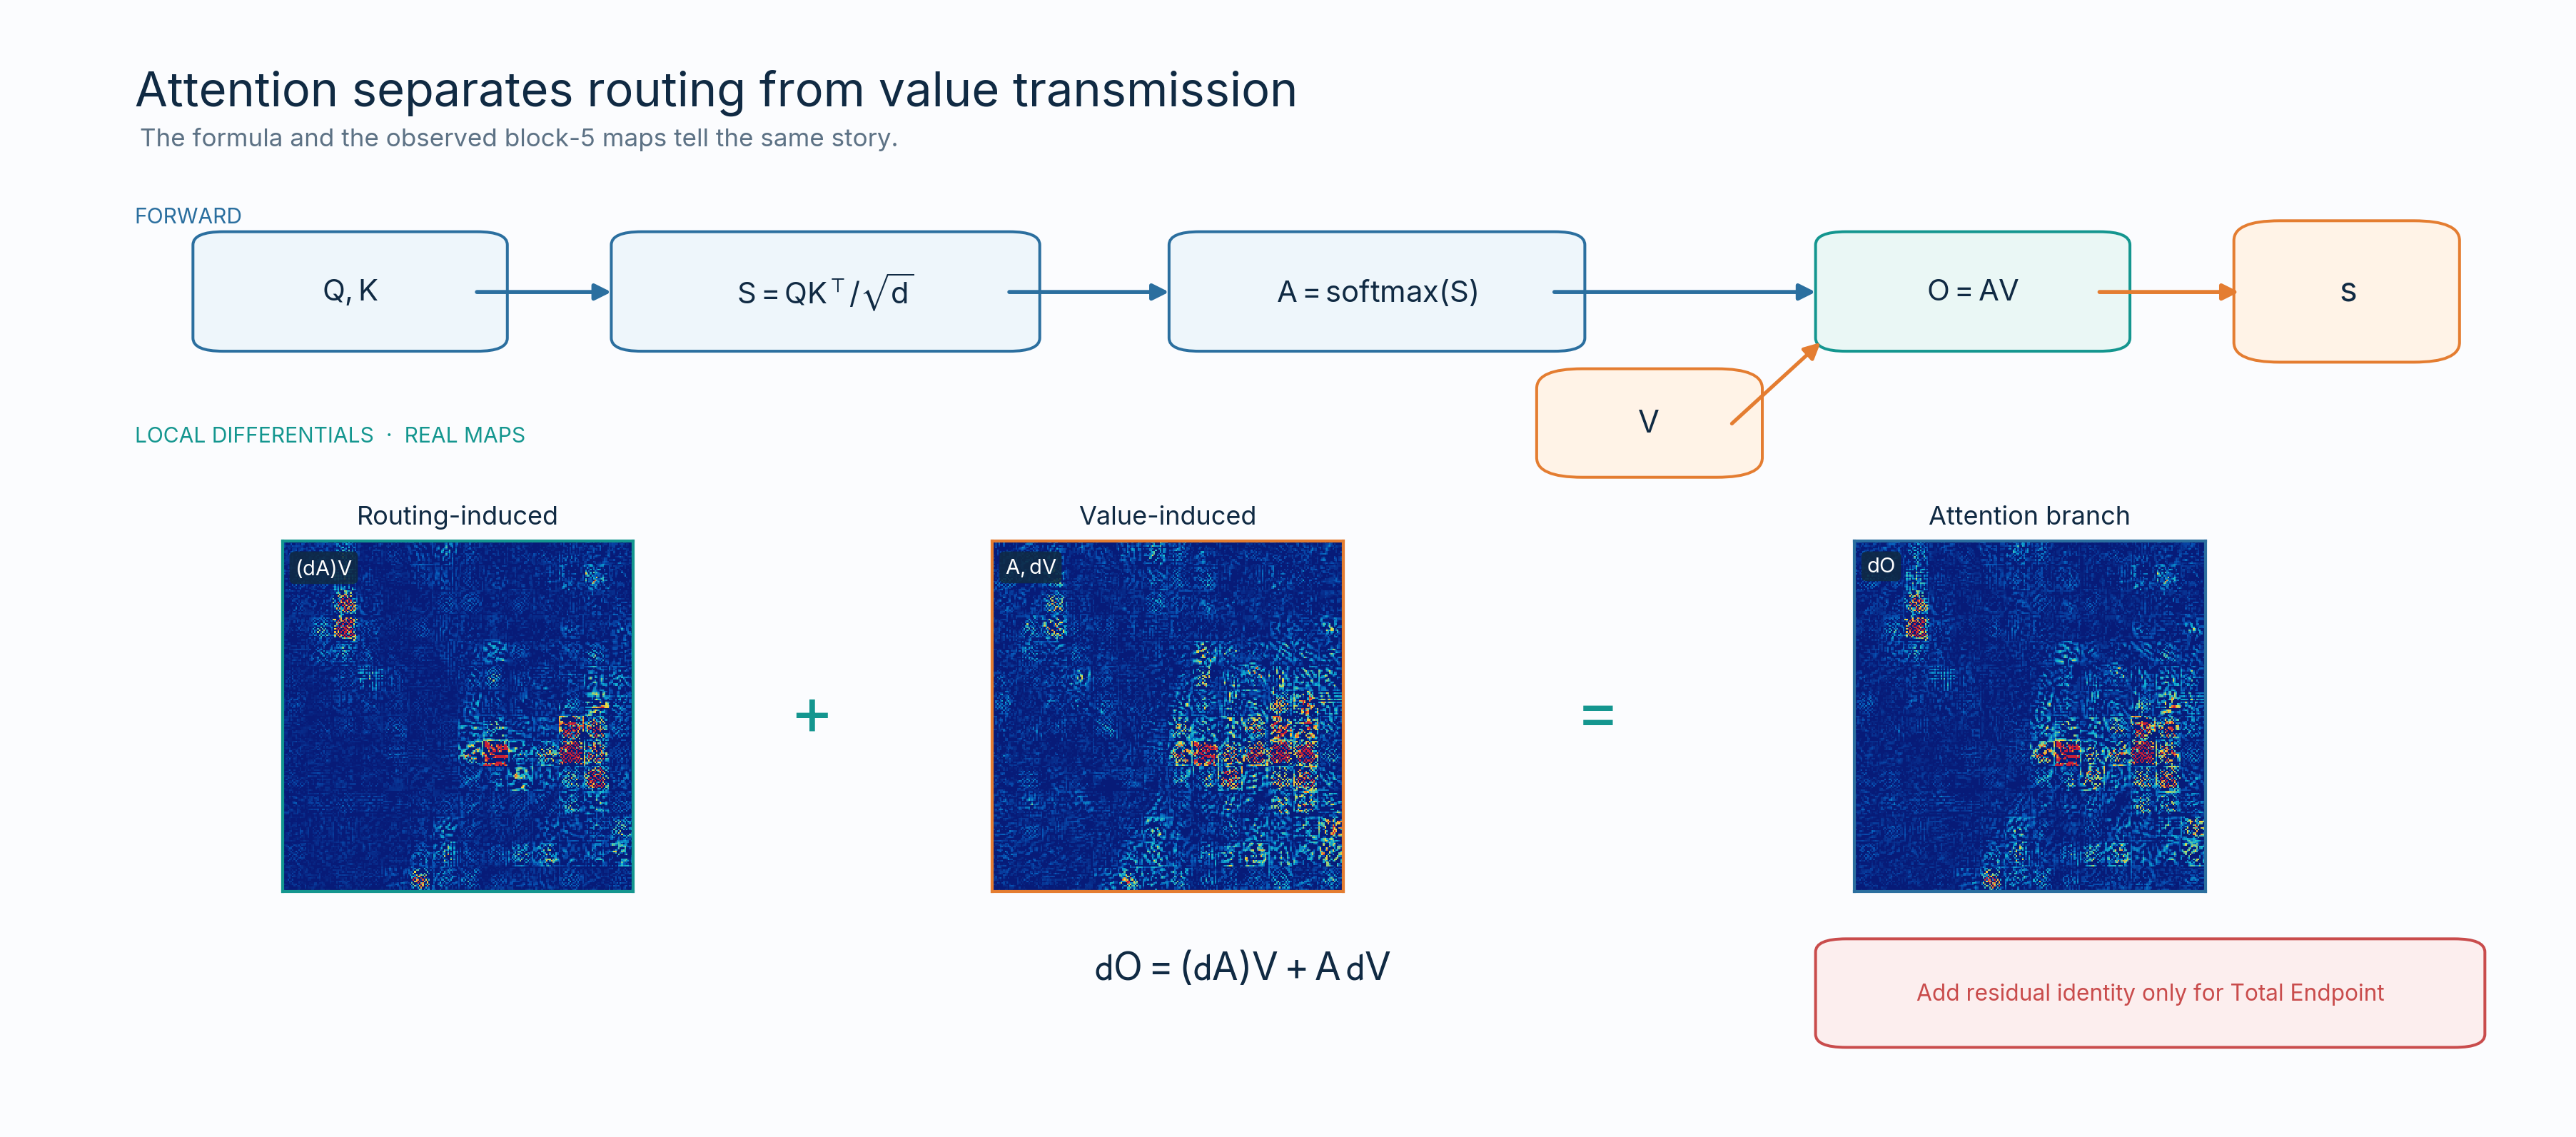
\includegraphics[keepaspectratio,alt={Figure 3}]{../figures/png/fig_06_attention_differential.png}}

\textbf{Figure 3.} 上行是单个 head 的前向计算，\(A\) 为 attention
probability，\(V\) 为 value projection。下行在同一前向点分解
\(\mathrm dO_h=(\mathrm dA)V+A\mathrm dV\)。Q-induced 与 K-induced 合成
routing-induced differential，V-induced 为 value-induced
differential。各 head 经 concat 和 output projection 的下游 cotangent
收缩后，分组重构 attention branch contribution。全局目标还需 residual
bypass。

\refstepcounter{figure}\label{fig:zh-manuscript-004}
\pandocbounded{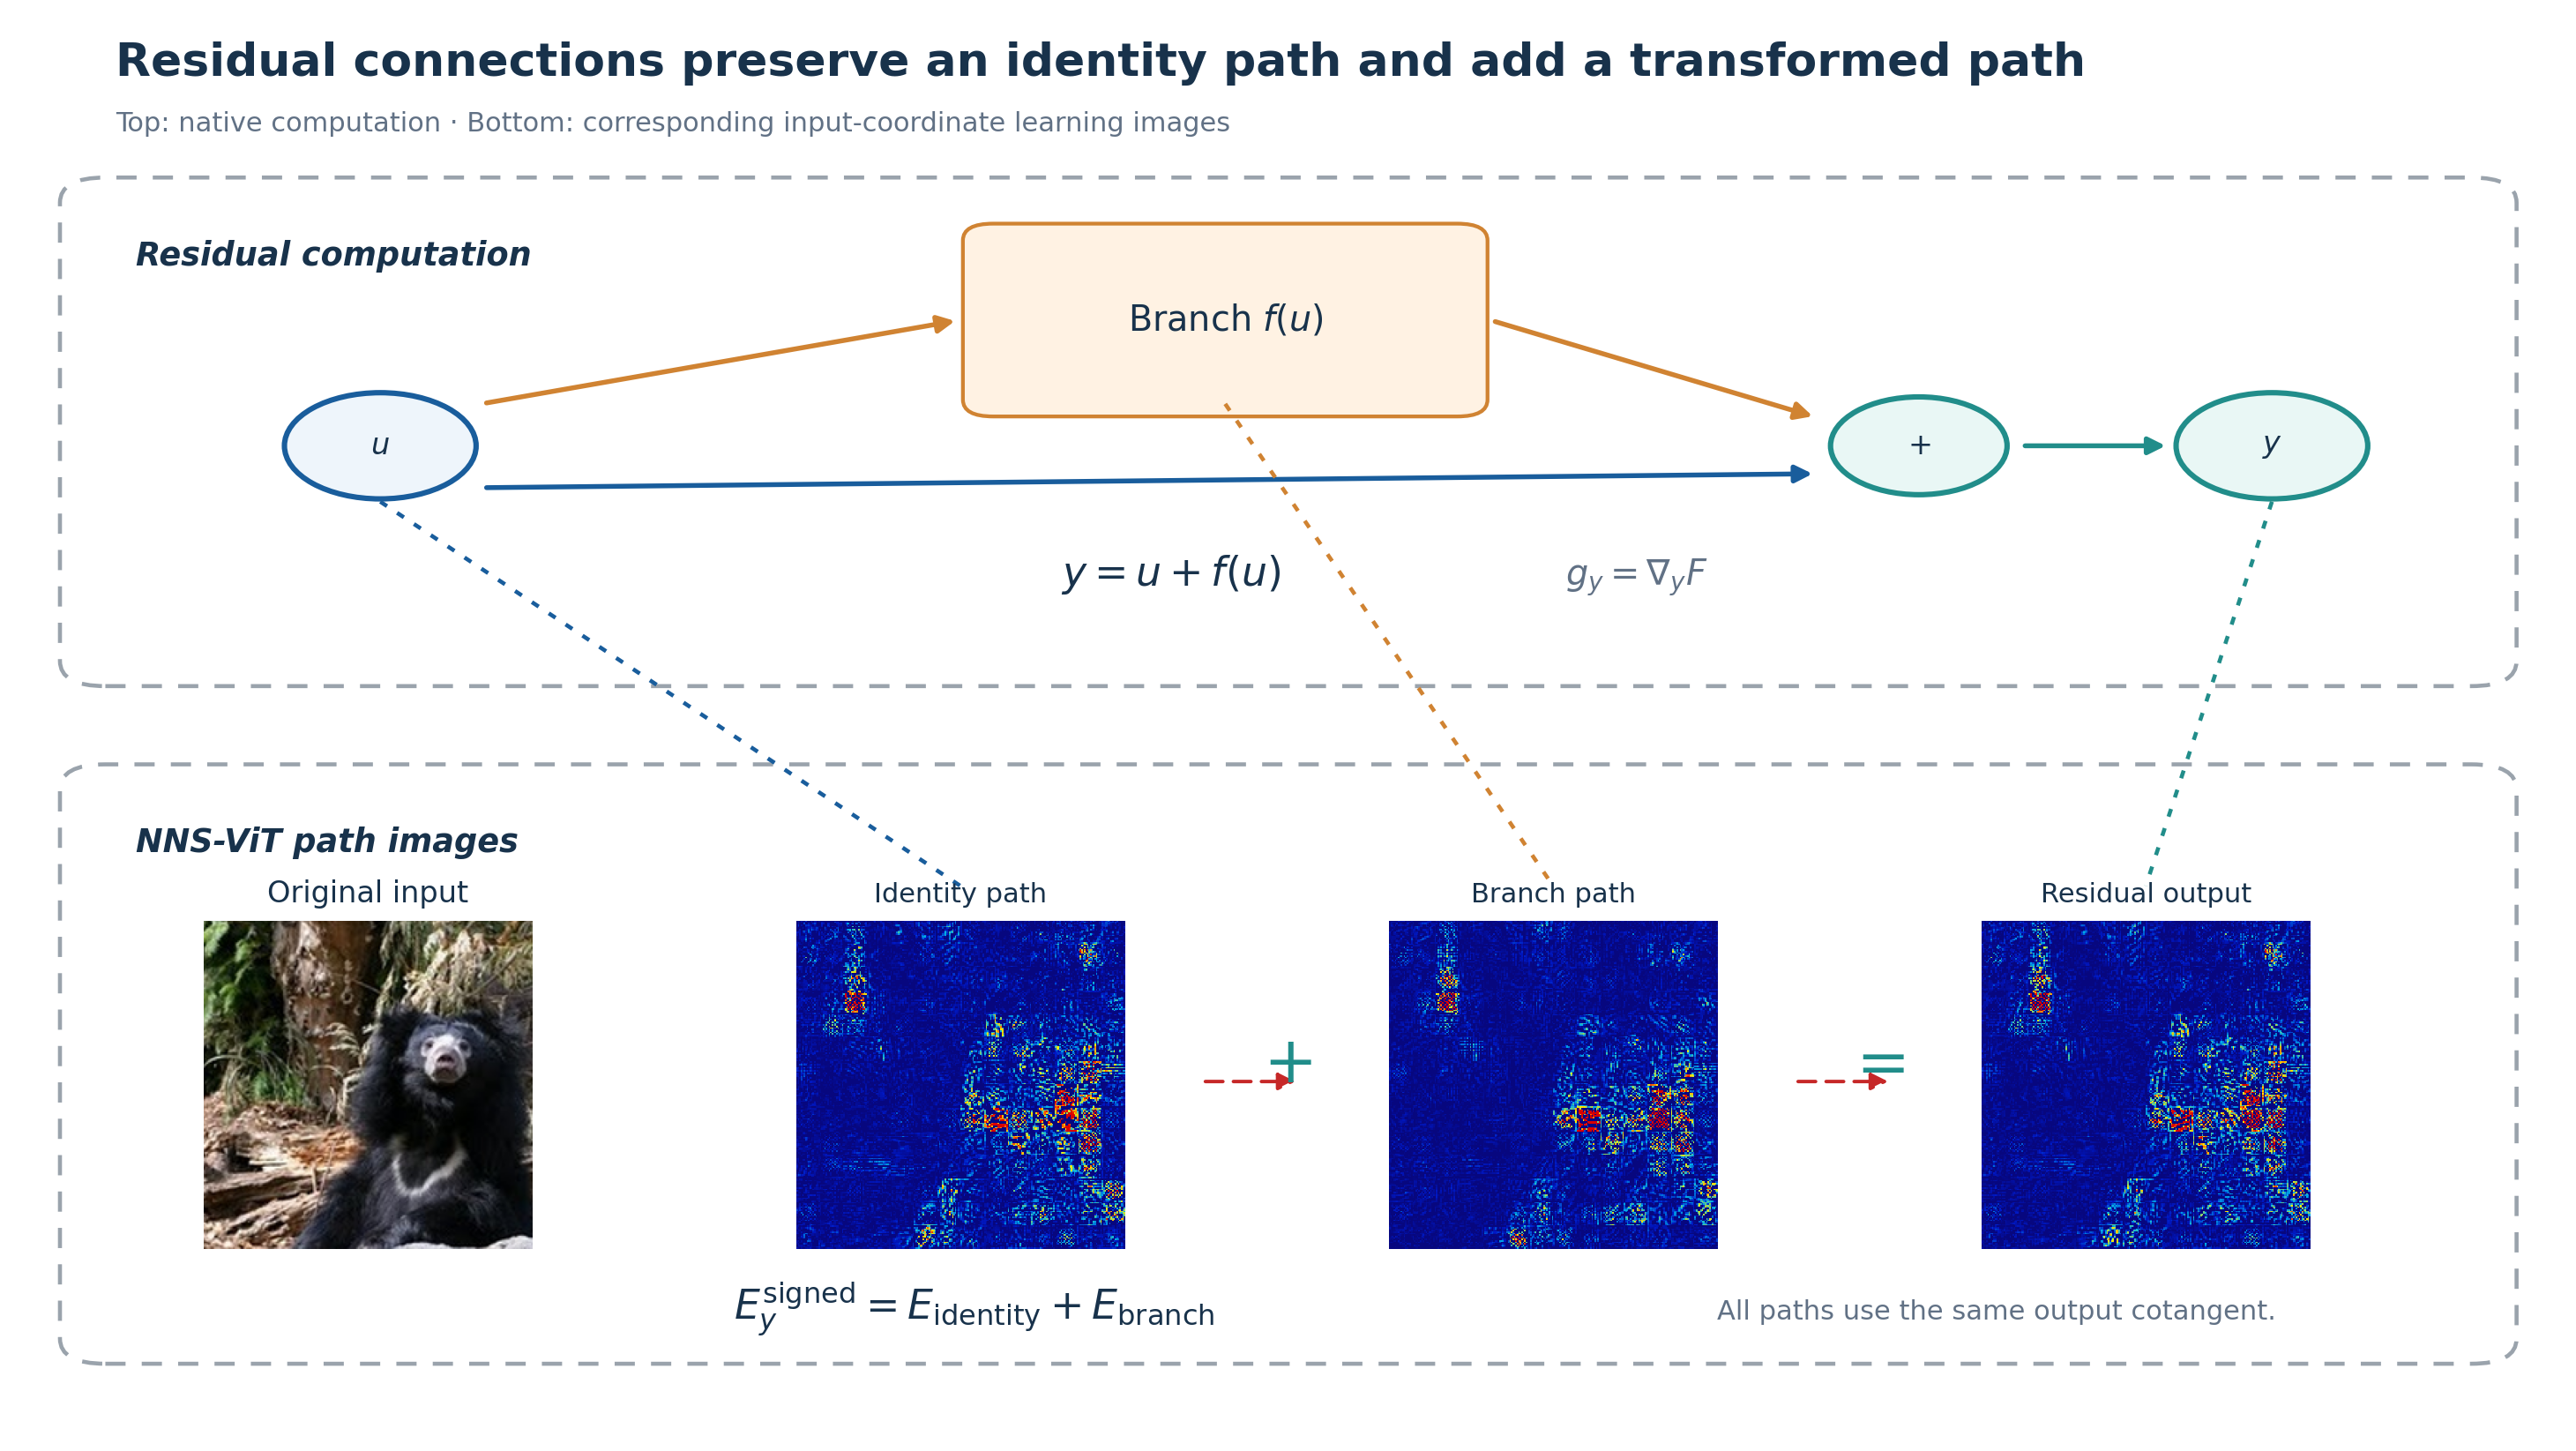
\includegraphics[keepaspectratio,alt={Figure 4}]{../figures/png/fig_07_residual_principle.png}}

\textbf{Figure 4.} Residual addition 的 identity 与 branch
输入分别定义局部图。二者使用同一最终类别目标和 addition 输出
cotangent。完整 signed 图之和为 Total
Endpoint；蓝底正部视图单独归一化，仅用于空间阅读。

对每个 head，\(Q=XW_Q+b_Q\)、\(K=XW_K+b_K\)、\(V=XW_V+b_V\)，且

\begin{equation}\label{eq:zh-manuscript-008}
A=\operatorname{softmax}(QK^\top/\sqrt{d_h}),\quad O_h=AV,\quad
\mathrm dO_h=(\mathrm dA)V+A\mathrm dV.
\end{equation}

这里
\(\mathrm dA=J_{\mathrm{softmax}}(S)\mathrm dS\)，\(\mathrm dS=(\mathrm dQK^\top+Q\mathrm dK^\top)/\sqrt{d_h}\)。令
attention branch 输出 \(a=f(u)\)，residual 输出 \(y=u+a\)，最终目标
\(s\) 在 \(y\) 处的 cotangent 为 \(g_y^{(s)}\)。定义

\begin{equation}\label{eq:zh-manuscript-009}
\mathcal B_i^{\mathrm{attn}}(s;x)
=x_i\left[J_{a,x}(x)^{\mathsf T}g_y^{(s)}\right]_i,
\qquad
\mathcal B_i^{\mathrm{attn}}
=\mathcal B_i^Q+\mathcal B_i^K+\mathcal B_i^V
=\mathcal B_i^{\mathrm{routing}}+\mathcal B_i^{\mathrm{value}}.
\end{equation}

Q/K/V projection slots 是原生计算图 use。Q-induced、K-induced 和
V-induced 是由这些 slots 的局部导数诱导的分项。Routing-induced
differential 是 Q-induced 与 K-induced 的解析合组，value-induced
differential 是 \(A\mathrm dV\)。这些 branch-internal differential
partitions 重构 attention branch contribution，单独不等于完整类别目标
G×I。每个 head map 的 cotangent 包含 concat、output projection \(W_O\)
和到最终目标的后续导数。各分项可在输入空间重叠。

对 residual identity 定义

\begin{equation}\label{eq:zh-manuscript-010}
\mathcal L_i^{\mathrm{identity}}=x_i[J_{u,x}^{\mathsf T}g_y^{(s)}]_i,
\qquad
E_{s,i}=x_i\frac{\partial s}{\partial x_i}
=\mathcal L_i^{\mathrm{identity}}+\mathcal B_i^{\mathrm{attn}}.
\end{equation}

Identity 必须使用 addition 输出处的 cotangent。用已包含 branch 的
\(\nabla_u s\) 替代会重复记账。第二处 residual 同理，carry 加 MLP branch
重构同一 Total Endpoint。表中分别列出数学对象及实际实现的闭合目标。

{\def\LTcaptype{none} % do not increment counter
\begingroup\scriptsize
\setlength{\tabcolsep}{2pt}
\begin{longtable}[]{@{}
  >{\raggedright\arraybackslash}p{(\linewidth - 8\tabcolsep) * \real{0.2000}}
  >{\raggedright\arraybackslash}p{(\linewidth - 8\tabcolsep) * \real{0.2000}}
  >{\raggedright\arraybackslash}p{(\linewidth - 8\tabcolsep) * \real{0.2000}}
  >{\raggedright\arraybackslash}p{(\linewidth - 8\tabcolsep) * \real{0.2000}}
  >{\raggedright\arraybackslash}p{(\linewidth - 8\tabcolsep) * \real{0.2000}}@{}}
\toprule\noalign{}
\begin{minipage}[b]{\linewidth}\raggedright
Object class
\end{minipage} & \begin{minipage}[b]{\linewidth}\raggedright
Examples
\end{minipage} & \begin{minipage}[b]{\linewidth}\raggedright
Native forward tensor/use
\end{minipage} & \begin{minipage}[b]{\linewidth}\raggedright
Direct replacement
\end{minipage} & \begin{minipage}[b]{\linewidth}\raggedright
Reconstruction or estimand
\end{minipage} \\
\midrule\noalign{}
\endhead
\bottomrule\noalign{}
\endlastfoot
Native computational edge & Residual add identity/branch input;
head-to-concat input; Q/K/V projection slot & Yes & Only under a
specified runtime contract & Branch or full-target differential,
depending on the edge set \\
Analytic differential partition & Q-induced, K-induced, routing-induced,
value-induced terms & No; groups of derivative terms & No & Attention
branch contribution \\
Intervenable forward variable & Attention probability \(A\); value
projection \(V\); head output; residual branch activation & Yes & Yes &
Prescribed finite replacement effect \\
Aggregate or ranking score & Map absolute mass; regional map score;
reference-aware Taylor score & No & Not applicable & Specified
statistical estimand \\
\end{longtable}
\endgroup
}

{\def\LTcaptype{none} % do not increment counter
\begingroup\scriptsize
\setlength{\tabcolsep}{2pt}
\begin{longtable}[]{@{}
  >{\raggedright\arraybackslash}p{(\linewidth - 4\tabcolsep) * \real{0.3333}}
  >{\raggedright\arraybackslash}p{(\linewidth - 4\tabcolsep) * \real{0.3333}}
  >{\raggedright\arraybackslash}p{(\linewidth - 4\tabcolsep) * \real{0.3333}}@{}}
\toprule\noalign{}
\begin{minipage}[b]{\linewidth}\raggedright
Named component set
\end{minipage} & \begin{minipage}[b]{\linewidth}\raggedright
Required terms
\end{minipage} & \begin{minipage}[b]{\linewidth}\raggedright
Reconstruction target
\end{minipage} \\
\midrule\noalign{}
\endhead
\bottomrule\noalign{}
\endlastfoot
heads\_branch & All head maps & Attention branch contribution
\(\mathcal B^{\mathrm{attn}}\) (\(A_F\) in code) \\
qkv\_branch & Q-induced + K-induced + V-induced & Attention branch
contribution \(\mathcal B^{\mathrm{attn}}\) (\(A_F\)) \\
routing\_value\_branch & routing-induced + value-induced & Attention
branch contribution \(\mathcal B^{\mathrm{attn}}\) (\(A_F\)) \\
heads\_with\_bypass / qkv\_with\_bypass / routing\_value\_with\_bypass &
Identity + the corresponding complete branch partition & Total Endpoint
\(E_s\) (\(L_F\) in code) \\
residual1 / residual2 & Identity + attention / carry + MLP & Total
Endpoint \(E_s\) (\(L_F\)) \\
\end{longtable}
\endgroup
}

\subsection{4.3
结构合法切面与点态微分闭合}\label{ux7ed3ux6784ux5408ux6cd5ux5207ux9762ux4e0eux70b9ux6001ux5faeux5206ux95edux5408}

对指定的 tensor-use DAG、输入节点 \(x\) 和标量目标 \(s\)，令 \(C\)
为实际 use edge 集合。若在目标的输入祖先子图中，每条从 \(x\) 到 \(s\)
的有向 use-path 恰好穿过 \(C\) 中一条边，则 \(C\)
是相对于该图和目标的\textbf{结构合法切面}。该性质只由图结构、目标位置和
use 身份决定，与当前输入数值或当前点导数是否为零无关。

在固定输入、参数和导数约定下，若 use-specific cotangent 分组满足

\begin{equation}\label{eq:zh-manuscript-011}
\nabla_x s=\sum_{e\in C}J_{z_e,x}^{\mathsf T}\bar z_e^{(s)},
\end{equation}

则称 \(C\)
在该点对目标形成\textbf{点态微分闭合}。数值闭合只检查该点上的实现一致性；它不能发现一条结构存在但恰在当前点具有零导数的遗漏路径。

\textbf{命题 2（结构合法切面充分保证点态微分闭合）。}
设标量目标位于切面下游，从输入到该目标的全部结构路径都经过所声明切面。若计算图在
\(x\) 处按固定导数约定可微，各成分使用同一前向状态，且 \(C\)
是该目标祖先子图中的结构合法切面，则对每个输入坐标 \(i\)，

\begin{equation}\label{eq:zh-manuscript-012}
\boxed{
\sum_{e\in C^{\mathrm{global}}}\mathcal L_{e,i}(s;x)
=x_i\frac{\partial s(x)}{\partial x_i}.
}
\end{equation}

多输入算子的输入边分别计入；同一张量被多次使用时按四元组 \(e\) 而不是
tensor name
区分。命题不适用于切面下游、切面之外或有输入路径绕过该切面的目标。

\textbf{证明。} 将切面上的 tensor uses 视为同一多变量映射
\(z_C(x)=(z_e(x))_{e\in C}\) 的分量，并在每个 consumer input slot
保留独立 cotangent。结构合法性保证目标祖先子图可写为
\(s=\tilde s(z_C(x))\)，且没有输入路径绕过 \(C\)，也没有路径在 \(C\)
中重复计数。多变量链式法则给出

\begin{equation}\label{eq:zh-manuscript-013}
\nabla_xs=J_{z_C,x}^{\mathsf T}\nabla_{z_C}\tilde s
=\sum_{e\in C}J_{z_e,x}^{\mathsf T}\bar z_e^{(s)}.
\end{equation}

其中 \(\bar z_e^{(s)}\) 是分配到该具体 use 的 cotangent；共享 producer
的不同 consumer、slot 或 invocation 不先合并。逐坐标乘以 \(x_i\)
即得所示 Endpoint
等式。把链式法则展开为坐标乘积时可以得到路径直觉，但证明不需要枚举张量计算图中的路径。只切
\(f(u)\) 会遗漏 \(y=u+f(u)\) 的 identity bypass；以已经包含 branch 的
\(\nabla_us\) 作为 identity 项后再加入 branch 则会重复计数。

最小反例为 \(s(x)=x+x^2\)。在 \(x=0\)
处，遗漏平方支路后保留支路的导数仍为
\(1=\mathrm ds/\mathrm dx\)，点态数值闭合误差为零；但该支路从 \(x\) 到
\(s\)
的结构路径仍存在，所以遗漏它的边集不是结构合法切面。这一区分阻止用单点数值相等反推结构完整。

\textbf{方法消融表：索引必要性与对象退化}

{\def\LTcaptype{none} % do not increment counter
\begingroup\scriptsize
\setlength{\tabcolsep}{2pt}
\begin{longtable}[]{@{}
  >{\raggedright\arraybackslash}p{(\linewidth - 6\tabcolsep) * \real{0.2500}}
  >{\raggedright\arraybackslash}p{(\linewidth - 6\tabcolsep) * \real{0.2500}}
  >{\raggedright\arraybackslash}p{(\linewidth - 6\tabcolsep) * \real{0.2500}}
  >{\raggedright\arraybackslash}p{(\linewidth - 6\tabcolsep) * \real{0.2500}}@{}}
\toprule\noalign{}
\begin{minipage}[b]{\linewidth}\raggedright
Retained structure
\end{minipage} & \begin{minipage}[b]{\linewidth}\raggedright
Observable
\end{minipage} & \begin{minipage}[b]{\linewidth}\raggedright
Lost when removed
\end{minipage} & \begin{minipage}[b]{\linewidth}\raggedright
Degeneration
\end{minipage} \\
\midrule\noalign{}
\endhead
\bottomrule\noalign{}
\endlastfoot
\([e,i]\) with registered \(s\) and valid \(C\) & Path-specific spatial
maps that reconstruct one total local differential & Nothing in the
declared object & Auditable dual-indexed map family \\
no \(i\) & Per-edge aggregate magnitude or score & Spatial allocation
and signed spatial cancellation & Edge scalar \\
no \(e\) & Total input-coordinate dependence & Routing/value, head, and
identity/branch identity & Total Gradient × Input \\
no registered \(s\) & Maps from ad hoc scalar readouts & Comparable
target semantics and reproducible atlas coverage & Unregistered target
collection \\
no valid-cut contract & Named component maps & Detection of omitted or
duplicated live paths & Unverified component list \\
\end{longtable}
\endgroup
}

该表给出结构消融而非经验性能消融。删除 \(i\)
后，空间扩展和同一路径的空间重分配不可见；删除 \(e\)
后，不同路径在总图中相加；删除 \(s\) 的 registry
后，跨目标比较失去固定语义；删除合法切面后，图组即使外观合理也不能证明不漏不重。

\textbf{结构审计覆盖}

{\def\LTcaptype{none} % do not increment counter
\begingroup\scriptsize
\setlength{\tabcolsep}{2pt}
\begin{longtable}[]{@{}
  >{\raggedright\arraybackslash}p{(\linewidth - 6\tabcolsep) * \real{0.2500}}
  >{\raggedright\arraybackslash}p{(\linewidth - 6\tabcolsep) * \real{0.2500}}
  >{\raggedright\arraybackslash}p{(\linewidth - 6\tabcolsep) * \real{0.2500}}
  >{\raggedright\arraybackslash}p{(\linewidth - 6\tabcolsep) * \real{0.2500}}@{}}
\toprule\noalign{}
\begin{minipage}[b]{\linewidth}\raggedright
Audit layer
\end{minipage} & \begin{minipage}[b]{\linewidth}\raggedright
Reconstruction / question
\end{minipage} & \begin{minipage}[b]{\linewidth}\raggedright
Direct evidence
\end{minipage} & \begin{minipage}[b]{\linewidth}\raggedright
Scope
\end{minipage} \\
\midrule\noalign{}
\endhead
\bottomrule\noalign{}
\endlastfoot
Formula identity & Same-target Total Endpoint & 5,000 numerical
comparisons; 88 operator directions & Declared exact local-derivative
rules \\
Branch closure & Attention branch contribution A\_F & 28,800
branch-partition closures & Fixed tested attention graphs \\
Global closure & Total Endpoint L\_F & 48,000 bypass-inclusive or
residual closures & Fixed tested global cuts \\
Existing mutations & Omitted head/routing, duplicate identity & 9,600 of
each error, all rejected & Three prescribed fault classes \\
Independent analytic reference & Q/K/V, routing/value, heads, identity,
branch, full & 32 component comparisons and 9 central-difference
directions & Three tiny attention/residual graphs; float64 \\
Use-identity mutations & Wrong slot and merged fan-out & Four mutations
rejected after correct controls pass & Shared-producer toy and Q/K slot
exchange \\
Numerical directions and summaries & Local correctness & 6,144 analytic
JVP; 384 attention-detach consistency checks; 230,400 summary fields &
Directional/summary checks, not fully independent component
construction \\
\end{longtable}
\endgroup
}

本轮解析实现独立于主扫描器，比较驱动调用真实扫描器逐项对照。其非零非对称
fixture 能区分错误 slot 和提前合并的
use。正确性结论限于已测图与故障类型。完整数组、每项误差和 mutation
记录见\href{supplement.md\#v6-coordinate}{补充 S17}。

\subsection{4.4
计算图依赖与分解非唯一性}\label{ux8ba1ux7b97ux56feux4f9dux8d56ux4e0eux5206ux89e3ux975eux552fux4e00ux6027}

命题 2 的闭合是相对于指定计算图、切面和内部坐标成立的。端到端函数及总
Endpoint
可以在等价重参数化下保持不变，但逐坐标或逐路径项不必保持不变。考虑
\(x=(x_1,x_2)^\top\)、隐藏变量 \(h=x\) 和输出
\(s=(1,1)h=x_1+x_2\)。按隐藏坐标切分时，两个路径图分别为

\begin{equation}\label{eq:zh-manuscript-014}
E_1=(x_1,0)^\top,\qquad E_2=(0,x_2)^\top.
\end{equation}

令可逆变换 \(R=\begin{bmatrix}1&1\\0&1\end{bmatrix}\)，并以
\(h'=Rh\)、\(w'=R^{-\top}(1,1)^\top=(1,0)^\top\) 重写同一函数
\(s=w'^\top h'\)。新隐藏坐标下的路径图变为

\begin{equation}\label{eq:zh-manuscript-015}
E'_1=(x_1,x_2)^\top,\qquad E'_2=(0,0)^\top.
\end{equation}

两种实现都有
\(E_1+E_2=E'_1+E'_2=(x_1,x_2)^\top\)，但分项不同。类似地，改变合法切面会改变被命名和汇总的路径组。因此本文的
Q/K/V、head 和 residual 图是对冻结 ViT
实现中指定真实边的分解，不是仅由端到端函数决定的唯一解释，也不具有一般实现不变性。数值闭合在所测图、切面和
mutation 类型上检查遗漏或重复，不证明该分解跨等价图表示唯一。

\subsection{4.5 质量、抵消与 Value-only
近似}\label{ux8d28ux91cfux62b5ux6d88ux4e0e-value-only-ux8fd1ux4f3c}

在原始 normalized-input RGB 张量坐标上，以像素 \(p\) 的 RGB absolute
mass

\begin{equation}\label{eq:zh-manuscript-016}
M(p)=\sum_{c\in\{R,G,B\}}|E_{p,c}|,
\end{equation}

作为主空间度量，并保留 \(M^+(p)=\sum_c\max(E_{p,c},0)\) 与
\(M^-(p)=\sum_c\max(-E_{p,c},0)\) 分析符号。Patch 质量为
\(m_j=\sum_{p\in P_j}M(p)\)，非零总质量时归一化为
\(p_j=m_j/\sum_km_k\)；零质量样本传播为 NA，不用 \(\varepsilon\)
伪造分布。定义归一化空间熵 \(H=-\sum_jp_j\log p_j/\log196\)。Patch-token
的 own-token locality 取目标 patch 的 Chebyshev 半径 1
邻域质量并减去同面积均匀基线，CLS 不计算该指标；normalized distance
以目标 patch 到其他 patch 中心的欧氏距离除以 \(13\sqrt2\)
后作质量加权平均。

对完整 RGB 张量另定义
\(m(E)=\sum_i|E_i|\)、\(a(E)=\sum_iE_i\)。单图抵消和两路径抵消分别为

\begin{equation}\label{eq:zh-manuscript-017}
C^{\mathrm{map}}=1-\frac{|\sum_iE_i|}{\sum_i|E_i|},\qquad
C^{\mathrm{path}}=1-\frac{\|E^{(1)}+E^{(2)}\|_1}{\|E^{(1)}\|_1+\|E^{(2)}\|_1}.
\end{equation}

Routing scale 为
\(\|E^{\mathrm{routing}}\|_1/(\|E^{\mathrm{routing}}\|_1+\|E^{\mathrm{value}}\|_1)\)；identity
scale 同理。除比例外，实验同时报告 routing/value/full 与
identity/branch/output 的 absolute mass。Value-only 近似保留
\(A\mathrm dV\)，遗漏 \((\mathrm dA)V\)，其 Endpoint 相对误差为
\(\|E^{\mathrm{full}}-E^V\|_2/\|E^{\mathrm{full}}\|_2\)；JVP discrepancy
在冻结方向上使用对应的完整方向响应为分母。约 0.95
的误差表示与完整响应同量级的差异。

这些 scale 都是当前点局部微分的 absolute-mass
比，不是因果贡献率或功能权重。Own-token locality 的 Chebyshev 半径 1
对应 14×14 patch 网格上的一步邻域；半径 0/1/2
的事后敏感性只检查这一描述性选择。

统计在完整 signed RGB 张量上计算，零分母或零范数记为
NA。蓝底显示规则在实验设置中说明。

\subsection{4.6 有限替换与区域诱导的指定-head activation
替换}\label{ux6709ux9650ux66ffux6362ux4e0eux533aux57dfux8bf1ux5bfcux7684ux6307ux5b9a-head-activation-ux66ffux6362}

成分有限效应定义为
\(e_k=s(x)-s(x;z_k\leftarrow z_k^{\mathrm{ref}})\)。Table 6 比较图内
\(m_k\) 与 \(|e_k|\) 的 Spearman 相关。可替换变量是 attention
probability \(A\)、value projection \(V\)、head output 和 residual
branch activation。Routing-induced 与 value-induced differential
仅提供相应局部图，不能作为前向张量替换。

统一使用五类名称。Total Endpoint 是完整目标图 \(E_s\)。Edge-conditioned
local map 是固定 use 的 \(\mathcal L_{e,:}\)。Branch contribution map
是完整 branch partition 的加和。Regional map score
在候选区域内汇总指定图。Reference-aware Taylor score 使用 clean
cotangent 和实际 activation displacement。Tables 6--10
使用以下公式，其中 \(k\) 可以指原生 use 或已声明微分分组，\(x_P\)
只在区域 \(P\) 使用 reference 像素。

\begin{equation}\label{eq:zh-manuscript-018}
E_s=x\odot\nabla_xs,\qquad
m_k=\sum_i|\mathcal L_{k,i}|,\qquad
R_k(P)=\sum_{i\in P}|\mathcal L_{k,i}|,\qquad
R_{\mathrm{total}}(P)=\sum_{i\in P}|E_{s,i}|,
\end{equation}

\begin{equation}\label{eq:zh-manuscript-019}
R_{\nabla_x}(P)=\sum_{i\in P}|\partial_i s|,\qquad
T_k=\left|\langle g_k,z_k(x)-z_k^{\mathrm{ref}}\rangle\right|,\qquad
T_k(P)=\left|\langle g_k,z_k(x)-z_k(x_P)\rangle\right|.
\end{equation}

{\def\LTcaptype{none} % do not increment counter
\begingroup\scriptsize
\setlength{\tabcolsep}{2pt}
\begin{longtable}[]{@{}
  >{\raggedright\arraybackslash}p{(\linewidth - 4\tabcolsep) * \real{0.3333}}
  >{\raggedright\arraybackslash}p{(\linewidth - 4\tabcolsep) * \real{0.3333}}
  >{\raggedright\arraybackslash}p{(\linewidth - 4\tabcolsep) * \real{0.3333}}@{}}
\toprule\noalign{}
\begin{minipage}[b]{\linewidth}\raggedright
Table
\end{minipage} & \begin{minipage}[b]{\linewidth}\raggedright
Method or quantity
\end{minipage} & \begin{minipage}[b]{\linewidth}\raggedright
Formula and information
\end{minipage} \\
\midrule\noalign{}
\endhead
\bottomrule\noalign{}
\endlastfoot
6 & Component-map association & Spearman\((m_k,\lvert e_k\rvert)\) over
the fixed component family within each image; clean-only map mass \\
7 & Local-map / Taylor head rank & Rank \(m_k\) / \(T_k\); Capture@K is
top-K absolute effect divided by the candidate top-K effect; Regret@1 is
the best minus selected effect \\
8 & Paired regional AUC difference & AUC ranked by \(R_k\) minus AUC
ranked by \(R_{\mathrm{total}}\), \(R_{\nabla_x}\), \(T_k(P)\), or
random order \\
9 & Absolute isolated-effect AUC & Trapezoid over replaced area 0, 1/16,
2/16, 4/16; divide by 0.25; average heads within image \\
10 & Candidate regret / logit ratio &
\(1-\mathrm{AUC}/\mathrm{AUC}_{\mathrm{oracle}}\) /
\(\mathrm{AUC}/\lvert s(x)\rvert\); zero denominator is NA \\
\end{longtable}
\endgroup
}

Normalized-coordinate gradient baseline 使用 \(\nabla_xs\)，本文称为
normalized-coordinate gradient baseline。Raw-pixel gradient 为
\(\nabla_rs=\nabla_xs/\sigma\)，另在坐标敏感性中检查。区域任务固定 block
5 的三个 heads，共用 4×4 候选网格和 1、2、4 区域预算。Block 5
与每个模型的首、中、末 head 在结果访问前选定，用于覆盖该层的不同 head
索引，不代表全部 heads，也不是按效果筛选。先用混合输入获取目标 head
activation，再放入 clean forward；其他 heads 与 identity 保持
clean，替换后的下游节点全部重算。Random 对每次重复先取 absolute effect
并积分，再平均 20 次 AUC。Clean-only 图分数与 reference-aware Taylor
使用不同信息。比较估计的是指定 head 的两阶段 activation replacement
效应，不是总像素干预效应。

\href{supplement.md\#v6-intervention}{完整替换伪代码和变量表见补充
S16}。

\section{5.
实验设置与数值验证}\label{ux5b9eux9a8cux8bbeux7f6eux4e0eux6570ux503cux9a8cux8bc1}

\subsection{5.1 模型与图像}\label{ux6a21ux578bux4e0eux56feux50cf}

图像来自 ImageNet ILSVRC2012 的 50,000 图公开验证集，以官方 WNID
标签、原文件名、字节数和 SHA-256 标识。排除已有访问后，固定 SHA-256
排序选择 528 类各一图，分为 64 图 discovery、64 图 calibration 和 400 图
evaluation，三队列不重叠。100 图 unit study 是 evaluation
的固定子集，每层含 CLS、15 个分层 patch tokens 和 32 个 channels，共
6,144 个单元。正确性和置信度不参与入选，错误分类和低置信度图像均保留。

独立队列使用另 400 类各一图，与旧队列和同轮 500 图队列零重叠。四个公开
checkpoint
包括原模型与两个额外训练方案。它们是固定参数状态，非独立训练种子，也非团队外部复现。精确
timm
名称、训练来源、大小、SHA-256、重叠矩阵和随机规则见\href{supplement.md\#v6-data}{补充
S15}。

\refstepcounter{table}\label{tab:zh-manuscript-002}
\textbf{Table 2. 固定模型设置，描述性范围}

{\def\LTcaptype{none} % do not increment counter
\begingroup\scriptsize
\setlength{\tabcolsep}{2pt}
\begin{longtable}[]{@{}lll@{}}
\toprule\noalign{}
Model / setting & ViT-B/16 & DeiT-S/16 \\
\midrule\noalign{}
\endhead
\bottomrule\noalign{}
\endlastfoot
Blocks / heads / hidden dimension & 12 / 12 / 768 & 12 / 6 / 384 \\
Registered scalar targets/image & 457 & 385 \\
Evaluation images & 400 & 400 (same IDs) \\
Resize / crop & 248 / 224 & 248 / 224 \\
Normalization mean & {[}0.5, 0.5, 0.5{]} & {[}0.485, 0.456, 0.406{]} \\
Normalization std & {[}0.5, 0.5, 0.5{]} & {[}0.229, 0.224, 0.225{]} \\
\end{longtable}
\endgroup
}

\subsection{5.2 可视化设置}\label{ux53efux89c6ux5316ux8bbeux7f6e}

概念和层间图使用主体可辨的懒熊样本，方法对比另外使用螳螂和小蓝鹭。样本按展示可读性选择，总体结论仍来自完整样本。为对应学习图像与前向特征，每层按
patch activation 的空间方差选择通道，并将该通道的 energy
定义为标量目标。图中同时给出通道编号及实际 14×14 前向 feature
map；不同层可以选择不同通道。

主学习图像采用深蓝至青、黄、红的正部视图。设
\(P=\max(\sum_cE_c,0)\)，显示值为 \(\sqrt{\min(P/q_{.99},1)}\)，其中
\(q_{.99}\)
在正值像素上计算。该变换提高弱细节的可见性，并保持像素位置；它不参与任何统计。补充图件同时显示
signed 与 absolute 视图，并另列 patch-max
加双线性插值的显示变体，明确区分原生细粒度图与平滑区域图。

\subsection{5.3
统计总体与分析身份}\label{ux7edfux8ba1ux603bux4f53ux4e0eux5206ux6790ux8eabux4efd}

图像是主统计单位。图内按固定规则汇总，再用 10,000 次图像 bootstrap
给出中位数的逐项 95\% 区间。该 bootstrap 不产生 p 值，也不决定极小 p
值的分辨率。一类一图结果是对固定选样规则下类别---图像对的条件性重采样，不覆盖类内变异；独立
E5 队列与旧队列图像零重叠，不等于类别零重叠。区间条件于固定
checkpoint、目标集合、reference
和替换合同，不能直接推广到新神经元、heads 或架构。补充分析同时重采样
target strata 与图像。四 checkpoint
检查针对固定公开模型。区间为逐项区间，Holm 校正不将其变为同时区间。

原成分与区域研究共 28 项检验联合 Holm
校正。单元深度每模型五项，attention 每模型四项，residual
每模型和类型各两项。事后 residual TV 四项另作 Holm。独立队列 H1--H4
在每个 checkpoint
内校正四项。完整成员、冻结时间及身份见\href{supplement.md\#v6-data}{补充
S15}。这些本地计划在对应结果访问前冻结，未提供外部注册记录。

{\def\LTcaptype{none} % do not increment counter
\begingroup\scriptsize
\setlength{\tabcolsep}{2pt}
\begin{longtable}[]{@{}
  >{\raggedright\arraybackslash}p{(\linewidth - 16\tabcolsep) * \real{0.1111}}
  >{\raggedright\arraybackslash}p{(\linewidth - 16\tabcolsep) * \real{0.1111}}
  >{\raggedright\arraybackslash}p{(\linewidth - 16\tabcolsep) * \real{0.1111}}
  >{\raggedright\arraybackslash}p{(\linewidth - 16\tabcolsep) * \real{0.1111}}
  >{\raggedright\arraybackslash}p{(\linewidth - 16\tabcolsep) * \real{0.1111}}
  >{\raggedright\arraybackslash}p{(\linewidth - 16\tabcolsep) * \real{0.1111}}
  >{\raggedright\arraybackslash}p{(\linewidth - 16\tabcolsep) * \real{0.1111}}
  >{\raggedright\arraybackslash}p{(\linewidth - 16\tabcolsep) * \real{0.1111}}
  >{\raggedright\arraybackslash}p{(\linewidth - 16\tabcolsep) * \real{0.1111}}@{}}
\toprule\noalign{}
\begin{minipage}[b]{\linewidth}\raggedright
Analysis
\end{minipage} & \begin{minipage}[b]{\linewidth}\raggedright
Unit
\end{minipage} & \begin{minipage}[b]{\linewidth}\raggedright
Image-level value
\end{minipage} & \begin{minipage}[b]{\linewidth}\raggedright
Interval
\end{minipage} & \begin{minipage}[b]{\linewidth}\raggedright
Test
\end{minipage} & \begin{minipage}[b]{\linewidth}\raggedright
Sidedness
\end{minipage} & \begin{minipage}[b]{\linewidth}\raggedright
Zero handling
\end{minipage} & \begin{minipage}[b]{\linewidth}\raggedright
Multiplicity
\end{minipage} & \begin{minipage}[b]{\linewidth}\raggedright
Identity
\end{minipage} \\
\midrule\noalign{}
\endhead
\bottomrule\noalign{}
\endlastfoot
原成分关联 & image & 图内 Spearman\((m_k,|e_k|)\) & 10,000 次 percentile
bootstrap 中位数区间 & 精确符号检验 & 双侧 & \(|v|\le10^{-12}\) 为
tie；留在总样本和区间，排除于二项计数 & 与区域检验合计 28 项 Holm &
结果访问前本地冻结的主分析 \\
原区域比较 & image & 三个固定 heads 的配对 AUC 差 & 同上 & 精确符号检验
& 双侧 & 同上 & 同一 28 项 Holm & 结果访问前本地冻结的主分析 \\
H1--H4 & image & 每图固定聚合后的假设值 & 同上 & 精确符号检验 & 双侧 &
同上 & 每 checkpoint 四项 Holm & 预先规定的稳健性分析 \\
v7 分层诊断 & image & 分类型、分层或残差化相关 & 同上 &
若报告则为精确符号检验 & 双侧 & 同上 & 独立 post-hoc Holm family &
事后诊断 \\
\end{longtable}
\endgroup
}

精确符号检验的原假设是非零差中正负号概率相等。它直接检验符号概率；只有在相应分布条件下才可解释为中位数为零。正文表格的
p 值列明确为 Holm 调整后 p，机器证据保留原始值与全精度调整值。只有真实
Holm 调整值小于 \(10^{-6}\) 时才显示 \(p<10^{-6}\)。

0.10 相关和 0.05
区域增益是研究者设定的操作阈值。原复合条件要求完整尝试范围、至少 360
个有效图像、至少 300 个非零差、CI 宽度不超过
0.30/0.50、正点估计达到阈值、原 Holm p 不超过
0.05。区域条件还要求全部四基线通过。这与 CI 下限超过阈值不同。相关阈值
0.05/0.10/0.15 的点估计达标数为 12/11/9，CI 下限达标数为 12/10/7。相对
Taylor 或正确绝对值顺序随机基线的八项区域增益，在 0.025、0.05、0.10
下均未达标。敏感性分析不改变原冻结判断。

Table 3 报告固定数值测试的误差和覆盖，不作图像总体推断。原 float32
失败与同坐标 float64 复核均保留。

\refstepcounter{table}\label{tab:zh-manuscript-003}
\textbf{Table 3. 数值一致性与结构检查}

{\def\LTcaptype{none} % do not increment counter
\begingroup\scriptsize
\setlength{\tabcolsep}{2pt}
\begin{longtable}[]{@{}
  >{\raggedright\arraybackslash}p{(\linewidth - 6\tabcolsep) * \real{0.2500}}
  >{\raggedright\arraybackslash}p{(\linewidth - 6\tabcolsep) * \real{0.2500}}
  >{\raggedright\arraybackslash}p{(\linewidth - 6\tabcolsep) * \real{0.2500}}
  >{\raggedright\arraybackslash}p{(\linewidth - 6\tabcolsep) * \real{0.2500}}@{}}
\toprule\noalign{}
\begin{minipage}[b]{\linewidth}\raggedright
Compatible network
\end{minipage} & \begin{minipage}[b]{\linewidth}\raggedright
Max relative L2: float64
\end{minipage} & \begin{minipage}[b]{\linewidth}\raggedright
Max relative L2: float32
\end{minipage} & \begin{minipage}[b]{\linewidth}\raggedright
Comparisons
\end{minipage} \\
\midrule\noalign{}
\endhead
\bottomrule\noalign{}
\endlastfoot
fcn & 4.371e-16 & 1.964e-07 & 1,000 \\
cnn & 4.289e-16 & 2.189e-07 & 1,000 \\
cnn\_maxpool & 4.769e-16 & 2.427e-07 & 1,000 \\
residual\_mlp & 2.686e-16 & 2.155e-07 & 1,000 \\
residual\_cnn & 2.923e-16 & 1.692e-07 & 1,000 \\
\end{longtable}
\endgroup
}

{\def\LTcaptype{none} % do not increment counter
\begingroup\scriptsize
\setlength{\tabcolsep}{2pt}
\begin{longtable}[]{@{}lll@{}}
\toprule\noalign{}
Structural / directional check & Count & Result \\
\midrule\noalign{}
\endhead
\bottomrule\noalign{}
\endlastfoot
Positive closures & 76,800 & All pass \\
Omission/duplication controls & 28,800 & All rejected \\
Analytic JVP & 6,144 & All pass \\
Operator directions & 88 & All pass \\
Atlas float32 finite differences & 57,600 & 36 outside tolerance \\
Same-coordinate float64 review & 36 & All pass \\
\end{longtable}
\endgroup
}

\subsection{5.4
结果顺序与证据范围}\label{ux7ed3ux679cux987aux5e8fux4e0eux8bc1ux636eux8303ux56f4}

先报告身份和计算正确性，再报告 normalized-input Endpoint
的空间轨迹、独立队列检查和坐标敏感性，最后评价规定有限替换。闭合说明局部微分记账，空间分布是固定
checkpoint 的描述，替换效应则依赖具体 reference 与干预变量。

\section{6. ViT
内部局部依赖的层深分布轨迹}\label{vit-ux5185ux90e8ux5c40ux90e8ux4f9dux8d56ux7684ux5c42ux6df1ux5206ux5e03ux8f68ux8ff9}

\subsection{6.1 NNS
等价性与结构路径闭合}\label{nns-ux7b49ux4ef7ux6027ux4e0eux7ed3ux6784ux8defux5f84ux95edux5408}

Table 3 的 5,000 个原始 NNS 兼容网络比较表明，逐层 learning-image
propagation 与同目标 Input × Gradient 的最大 relative L2 error 在
float64 下不超过 \(4.769\times10^{-16}\)，在 float32 下不超过
\(2.427\times10^{-7}\)。结构验证进一步覆盖 76,800 项正向闭合、28,800
项遗漏/重复负控、6,144 项解析 JVP 和 88
个算子方向。所有正向闭合与解析方向检查通过，所有负控被拒绝；36 个
float32 有限差分超差点在相同坐标的 float64
复核中全部通过。这些结果分别建立命题 1 的数值身份和命题 2
的结构记账；有限干预效用由 Section 7 单独评价。

本轮独立解析参考的 32 个逐分量比较与 9
个中心有限差分方向均通过，最大分量绝对误差为
\(1.11\times10^{-16}\)。四类新增 use mutation 均拒绝，详见补充 S17。

\subsection{6.2
固定目标的空间分布}\label{ux56faux5b9aux76eeux6807ux7684ux7a7aux95f4ux5206ux5e03}

Figure 5 展示同一图像不同目标的 normalized-input Endpoint。前向 feature
描述 token-grid 响应，局部图描述该 scalar
对输入坐标缩放的当前点响应。总体统计使用固定抽样目标，不从展示图选择目标。

\refstepcounter{figure}\label{fig:zh-manuscript-005}
\pandocbounded{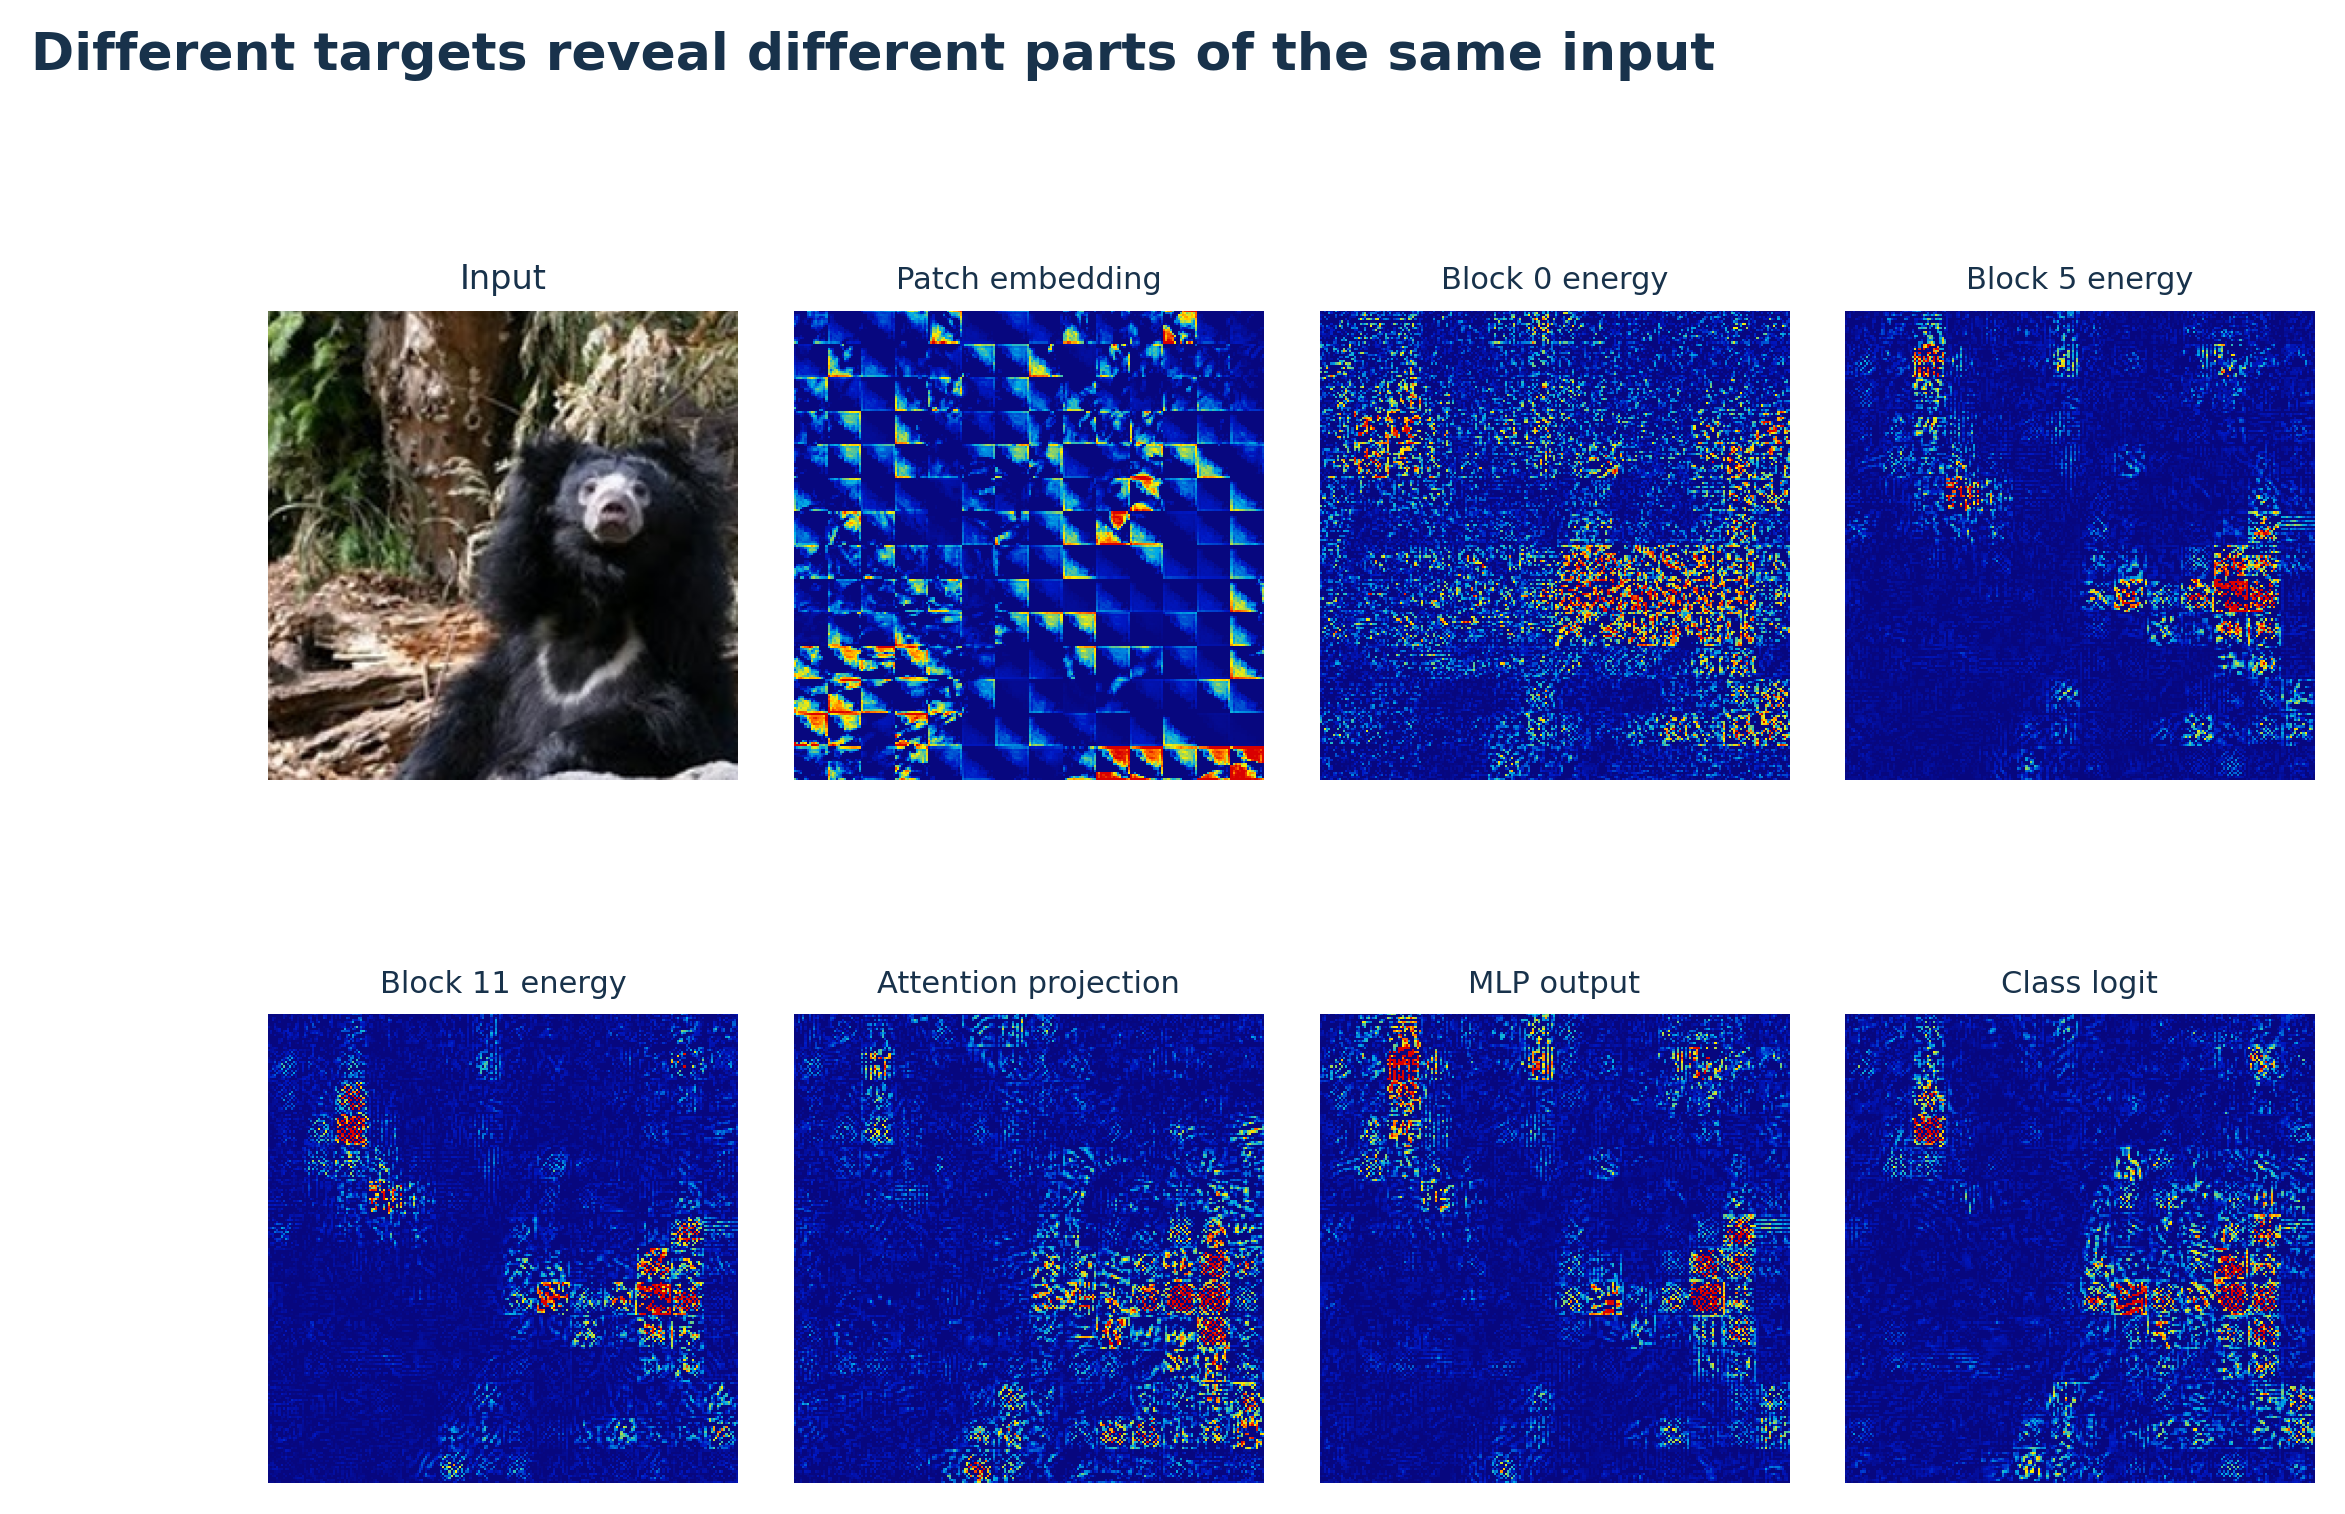
\includegraphics[keepaspectratio,alt={Figure 5}]{../figures/png/fig_08_internal_targets.png}}

\textbf{Figure 5.} 从左至右、从上至下为同一懒熊输入、patch embedding
energy、blocks 0/5/11 energy、block 5 attention projection energy、MLP
output energy 和 ground-truth class logit 的 normalized-input
Endpoint。模型为 DeiT-S/16。每个 energy 使用相应前向空间方差最大 channel
的半平方和目标。每个 map panel 取 signed RGB sum 的正部，以正值 P99
截断并开方，各 panel 独立缩放；单个展示样本，无统计区间或总体推断。

每模型 100 图的 late-minus-early 图像级中位差和 95\% 区间如下，顺序为
ViT-B/16 与 DeiT-S/16。entropy 0.220 {[}0.211, 0.227{]} / 0.225
{[}0.212, 0.228{]}；locality -0.356 {[}-0.363, -0.350{]} / -0.342
{[}-0.353, -0.333{]}；distance 0.131 {[}0.129, 0.136{]} / 0.122
{[}0.120, 0.128{]}。每图先在 blocks 8--11 与 0--3
的固定单元内分别取中位数，再求差。Locality 与 distance 排除 CLS。这是
normalized-input Endpoint 的分布轨迹，不识别深度的因果效应。

空间熵对低幅值的事后敏感性分析使用每个 model--block 的总 L1 mass
分位点，不按熵结果选阈值。剔除最低 1\%、5\% 和 10\% mass 后，ViT-B 的
late-minus-early entropy 中位差依次为 0.222、0.229 和 0.234，DeiT-S 为
0.226、0.230 和 0.233；各设置仍为 100/100
图像正向。按质量四分位分层后，两模型四组中位差均为正，最低质量组为 0.090
和 0.112。与此同时，同图同层 log1p(total mass) 与 entropy 的平均
Spearman 中位数为 −0.729 和
−0.760，表明熵确实依赖图质量；因此这里只支持空间扩展方向不由最低质量图单独驱动，而不将归一化熵解释为幅值无关量。完整区间、有效数和
8 个 typed-NA image--quartile 单元见补充 S19。

\refstepcounter{figure}\label{fig:zh-manuscript-006}
\pandocbounded{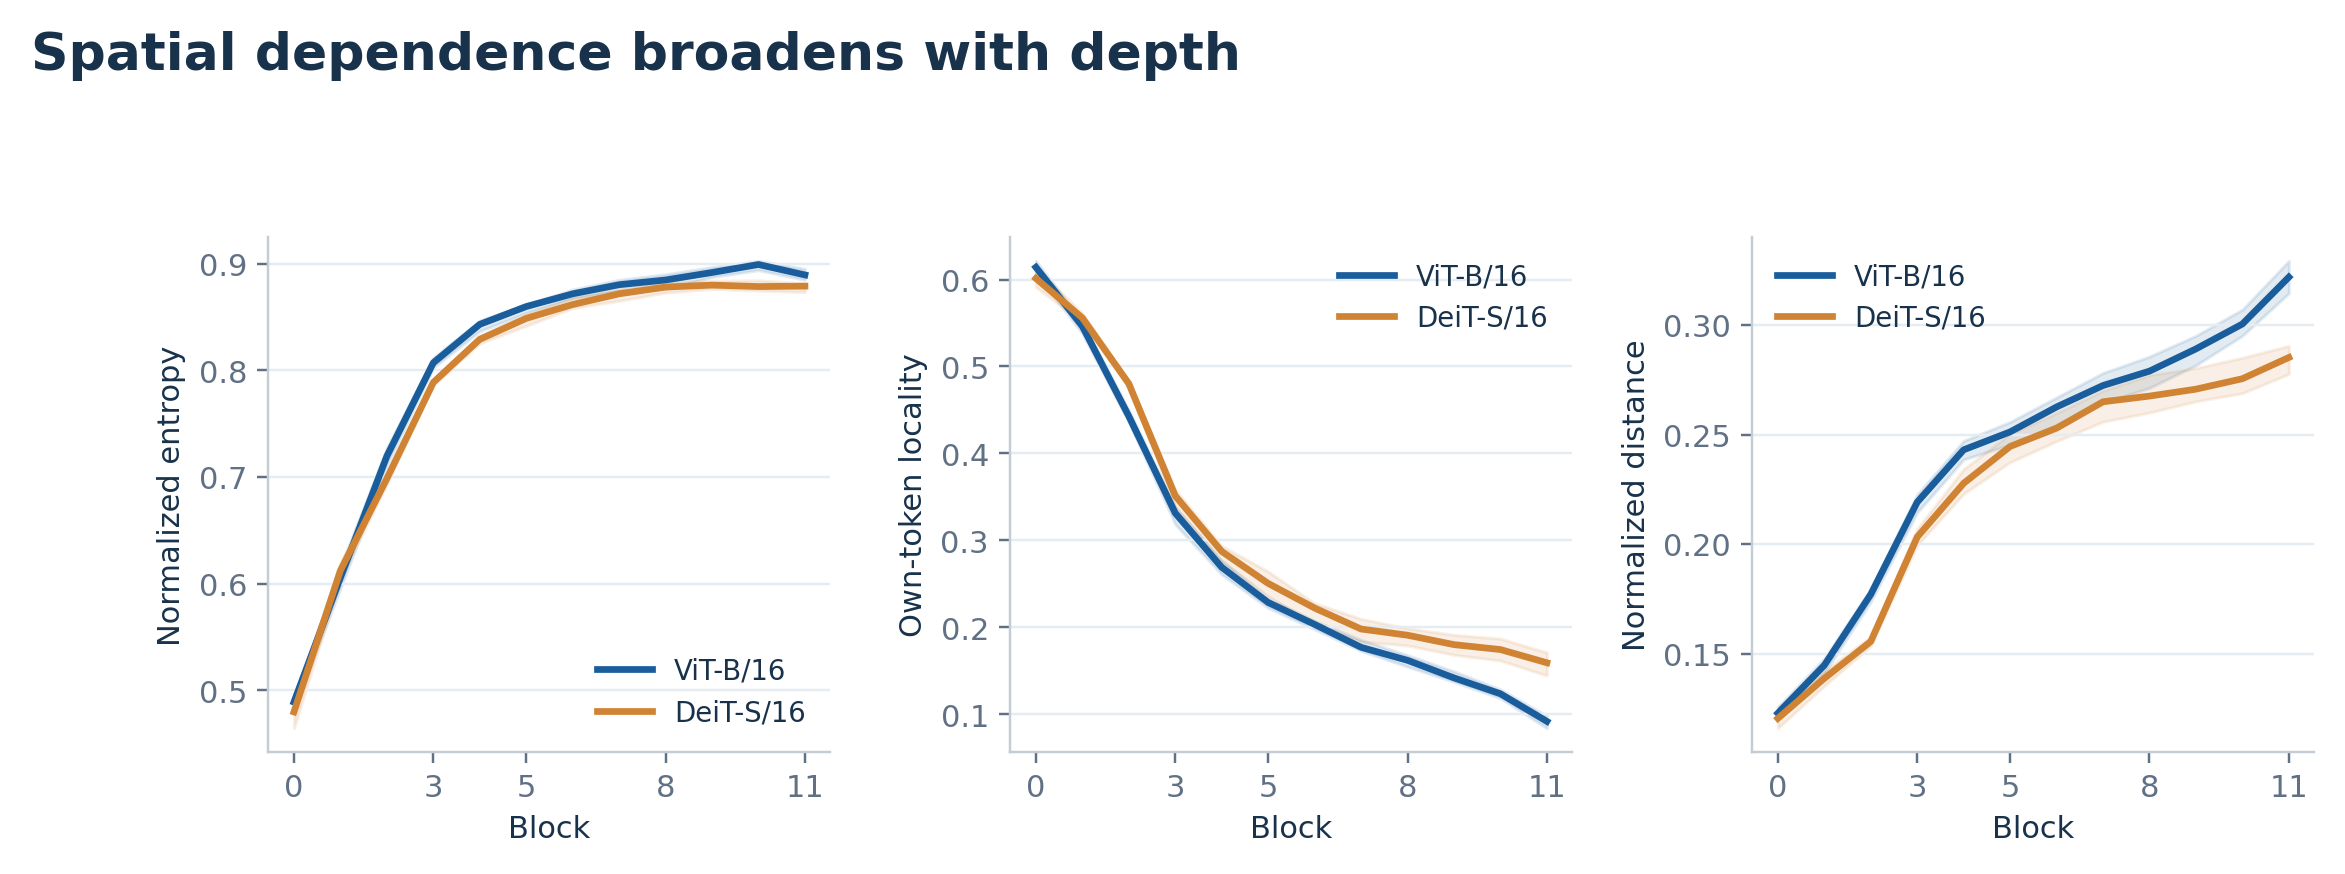
\includegraphics[keepaspectratio,alt={Figure 6}]{../figures/png/fig_12_spatial_broadening.png}}

\textbf{Figure 6.} 左、中、右 panel 分别为 normalized-input Endpoint
的空间熵、own-token locality 和 normalized distance。每个 block
先在图内取固定 token-channel 目标的中位数，再汇总 100 张 evaluation
子集图像的中位数。CLS 仅进入熵统计；locality 扣除同面积均匀基线。阴影为
10,000 次图像 bootstrap 的 95\% 区间。两条曲线对应两个固定
checkpoint。曲线为描述性 block 轨迹，late-minus-early
检验属于结果访问前冻结的五项 family。

\subsection{6.3
联合索引必要性}\label{ux8054ux5408ux7d22ux5f15ux5fc5ux8981ux6027}

总 Gradient × Input、edge scalar 和双索引图组保留的信息不同。Table 4
将三者对应到本文的实际结果。层深空间扩展只需要总图，因此作为背景规律；routing
share 与 identity share 只需要 edge-level absolute
mass，因此作为支持性尺度结果。Attention 的 Full--Value 空间差异和
residual 的 output--identity 空间差异同时要求路径身份 \(e\) 与输入位置
\(i\)，构成需要两个索引的空间结果。

\refstepcounter{table}\label{tab:zh-manuscript-004}
\textbf{Table 4. 表示信息与统计范围}

{\def\LTcaptype{none} % do not increment counter
\begingroup\scriptsize
\setlength{\tabcolsep}{2pt}
\begin{longtable}[]{@{}
  >{\raggedright\arraybackslash}p{(\linewidth - 6\tabcolsep) * \real{0.2500}}
  >{\raggedright\arraybackslash}p{(\linewidth - 6\tabcolsep) * \real{0.2500}}
  >{\raggedright\arraybackslash}p{(\linewidth - 6\tabcolsep) * \real{0.2500}}
  >{\raggedright\arraybackslash}p{(\linewidth - 6\tabcolsep) * \real{0.2500}}@{}}
\toprule\noalign{}
\begin{minipage}[b]{\linewidth}\raggedright
Representation
\end{minipage} & \begin{minipage}[b]{\linewidth}\raggedright
Retained indices
\end{minipage} & \begin{minipage}[b]{\linewidth}\raggedright
Recoverable quantity
\end{minipage} & \begin{minipage}[b]{\linewidth}\raggedright
Evidence / inference scope
\end{minipage} \\
\midrule\noalign{}
\endhead
\bottomrule\noalign{}
\endlastfoot
Total Endpoint & \(i\) & Entropy, locality, distance & 100 images/model;
fixed sampled targets; image-level inference \\
Component scalar & use or differential-group label & \(m_k\) and
relative mass & 400 images/model; fixed checkpoint and class target \\
Dual-indexed map set & label and \(i\) & Q/K/V entropy; output--identity
TV & 400 images/model; QKV prospective robustness; residual TV
post-hoc \\
\end{longtable}
\endgroup
}

替代解释审计采用与正文主张相同的信息边界。总图保留 \(i\) 但求和消去
\(e\)，不能恢复 routing/value 或 identity/branch 的分别空间分布；edge
scalar 保留 \(e\) 但求和消去 \(i\)，不能计算归一化 patch
distribution、spatial TV 或 signed spatial cancellation。总 absolute
mass 和 activation norm
可解释整体尺度，却不能重建这些位置条件差异。Full--Value 与
output--identity TV 均在各自绝对质量归一化后比较空间分布，因此不是总
mass 的重述。由此，空间重组结论依赖 \([e,i]\)；routing share、identity
share 和总体空间扩展均不单独承担联合索引必要性主张。

\subsection{6.4 Attention
分支的空间分项}\label{attention-ux5206ux652fux7684ux7a7aux95f4ux5206ux9879}

Figure 7 区分 Q-induced、K-induced、routing-induced 与 value-induced
differential。各项的完整 signed 图重构 attention branch
contribution，图中正部仅作显示。

\refstepcounter{figure}\label{fig:zh-manuscript-007}
\pandocbounded{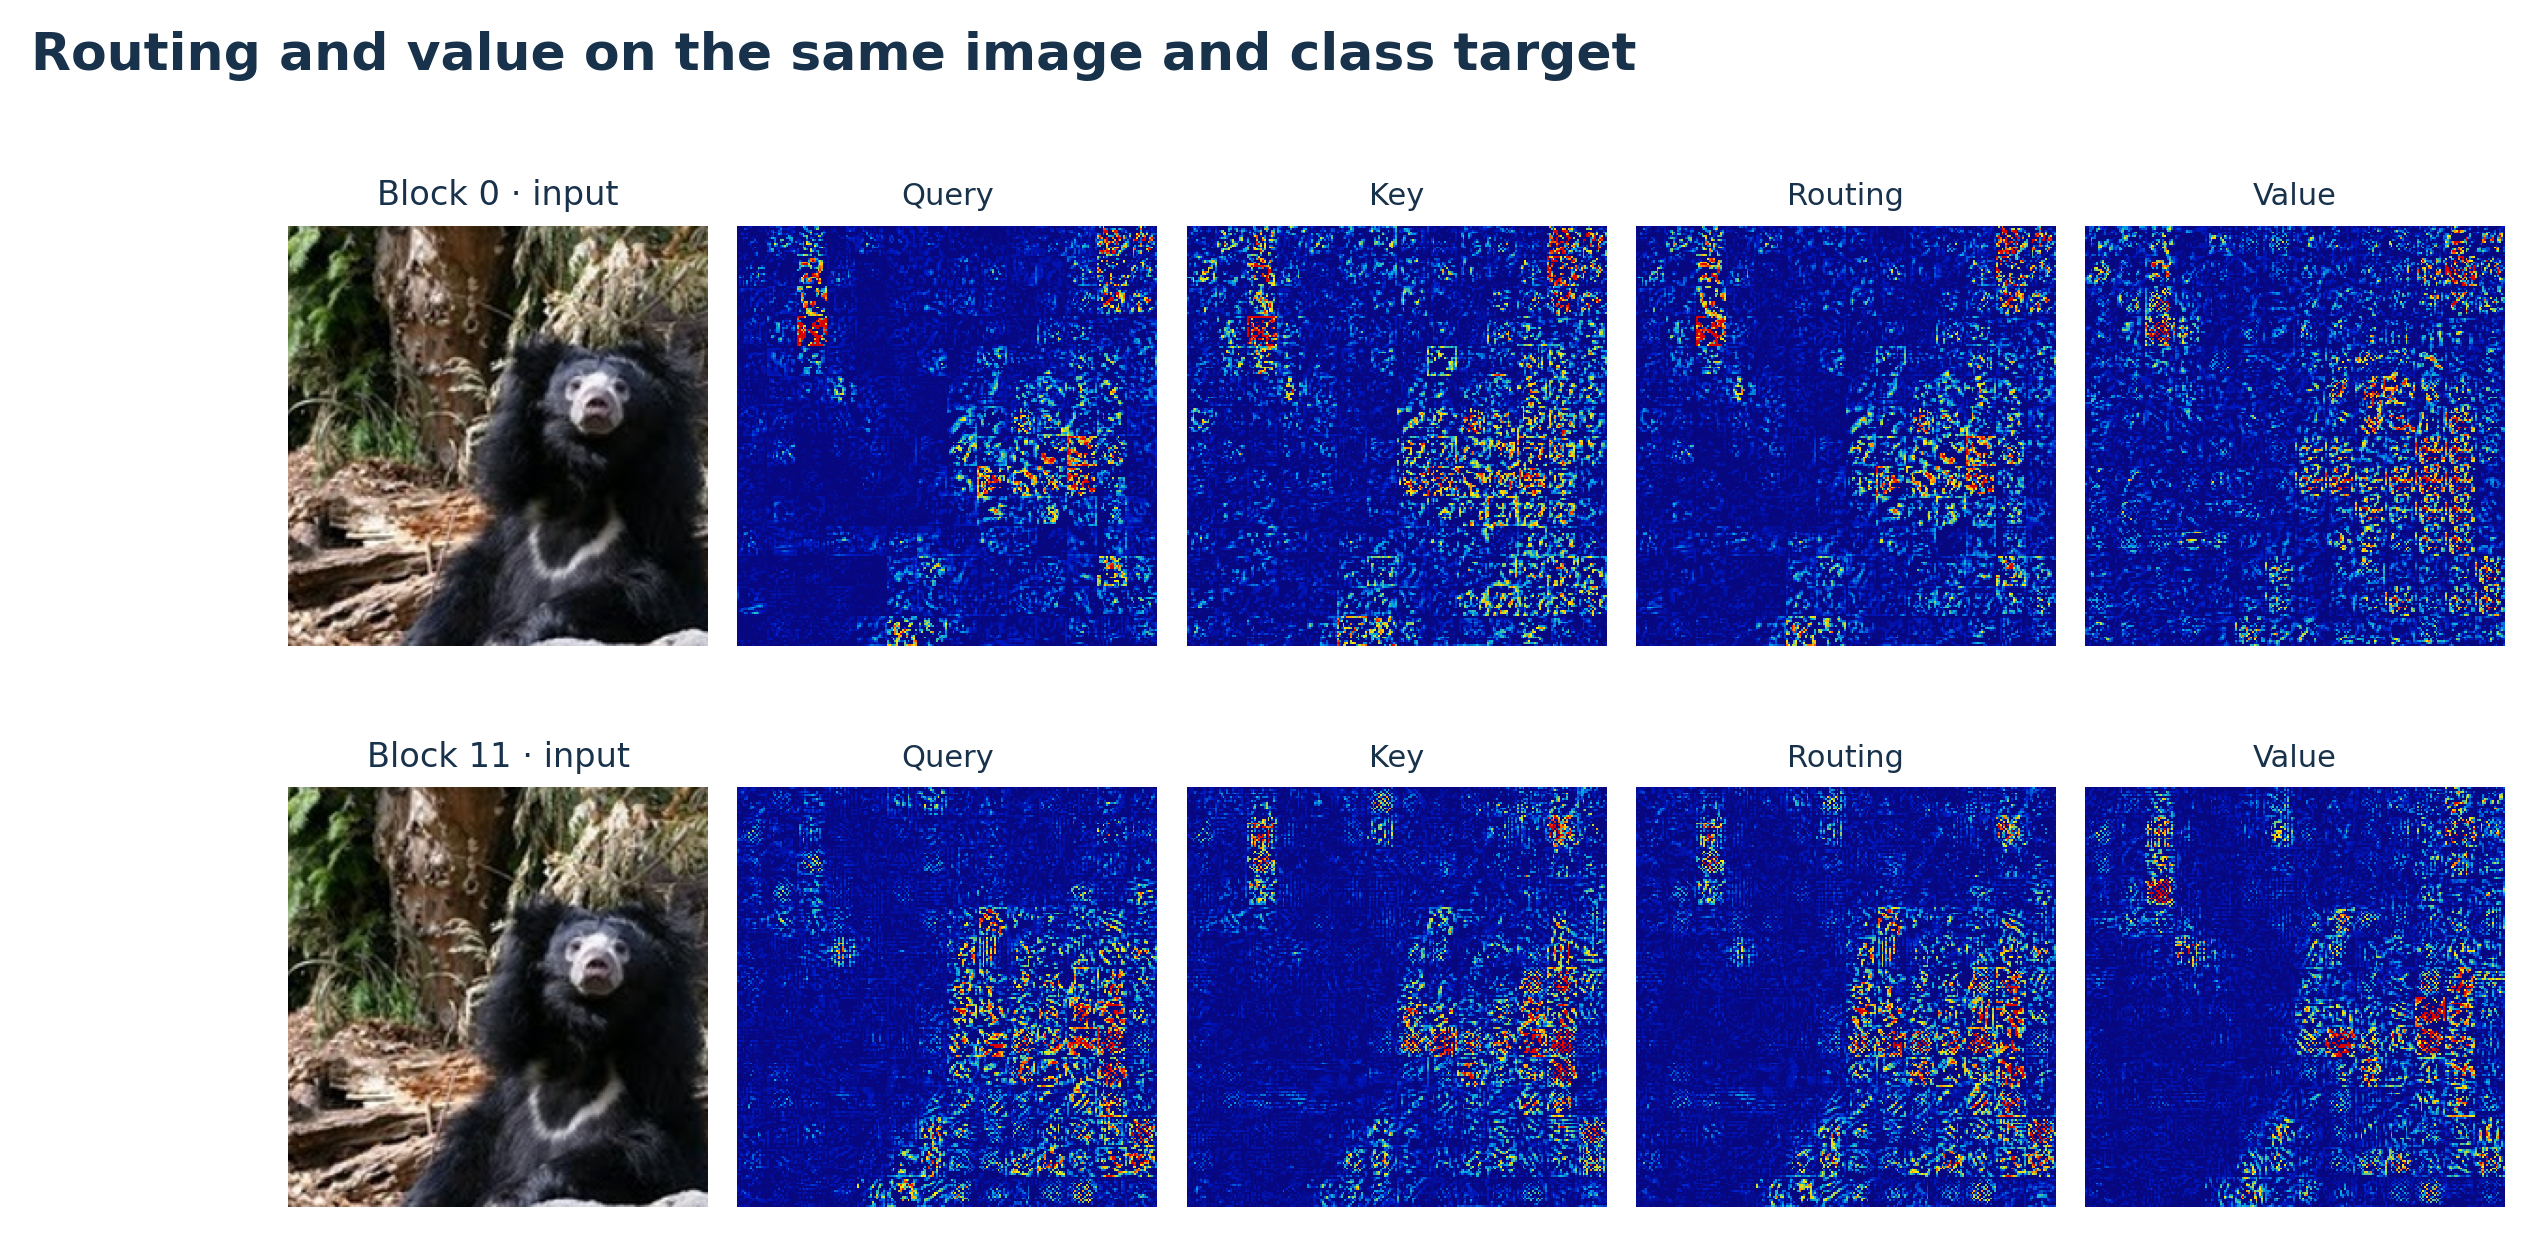
\includegraphics[keepaspectratio,alt={Figure 7}]{../figures/png/fig_15_routing_value_examples.png}}

\textbf{Figure 7.} 上下两行分别为 DeiT-S/16 blocks 0 和
11，同一懒熊输入和 ground-truth
logit。每行从左至右为输入、Q-induced、K-induced、routing-induced 与
value-induced 图，routing-induced 是 Q 与 K 图之和。图为
normalized-input 坐标的正部显示，正值 P99 截断、开方并独立缩放；没有跨
panel 幅值可比性。单例描述，无误差带。

每模型 400 图的 routing-relative local differential scale 随 block index
上升，late-minus-early 中位差为 0.052 {[}0.047, 0.059{]} / 0.135
{[}0.128, 0.143{]}。Value-only 相对完整 attention branch 图的 L2 error
增量为 0.144 {[}0.133, 0.152{]} / 0.290 {[}0.279,
0.301{]}。这些尺度量只需 component
scalar，空间分布比较则需保留输入位置。

Q/K/V 的完整 400 图对比为 B11−B0，不能与四层 phase medians
混用。Normalized entropy 的中位差和本轮描述性图像 bootstrap 区间为
vit\_b16: Q 0.027 {[}0.022, 0.031{]}, K -0.059 {[}-0.064, -0.053{]}, V
-0.053 {[}-0.059, -0.047{]}; deit\_s16: Q -0.004 {[}-0.008, 0.001{]}, K
-0.067 {[}-0.074, -0.059{]}, V -0.067 {[}-0.075, -0.061{]}。K/V
在两模型下降；Q 的模型依赖及 DeiT-S 跨零区间保留。

\refstepcounter{figure}\label{fig:zh-manuscript-008}
\pandocbounded{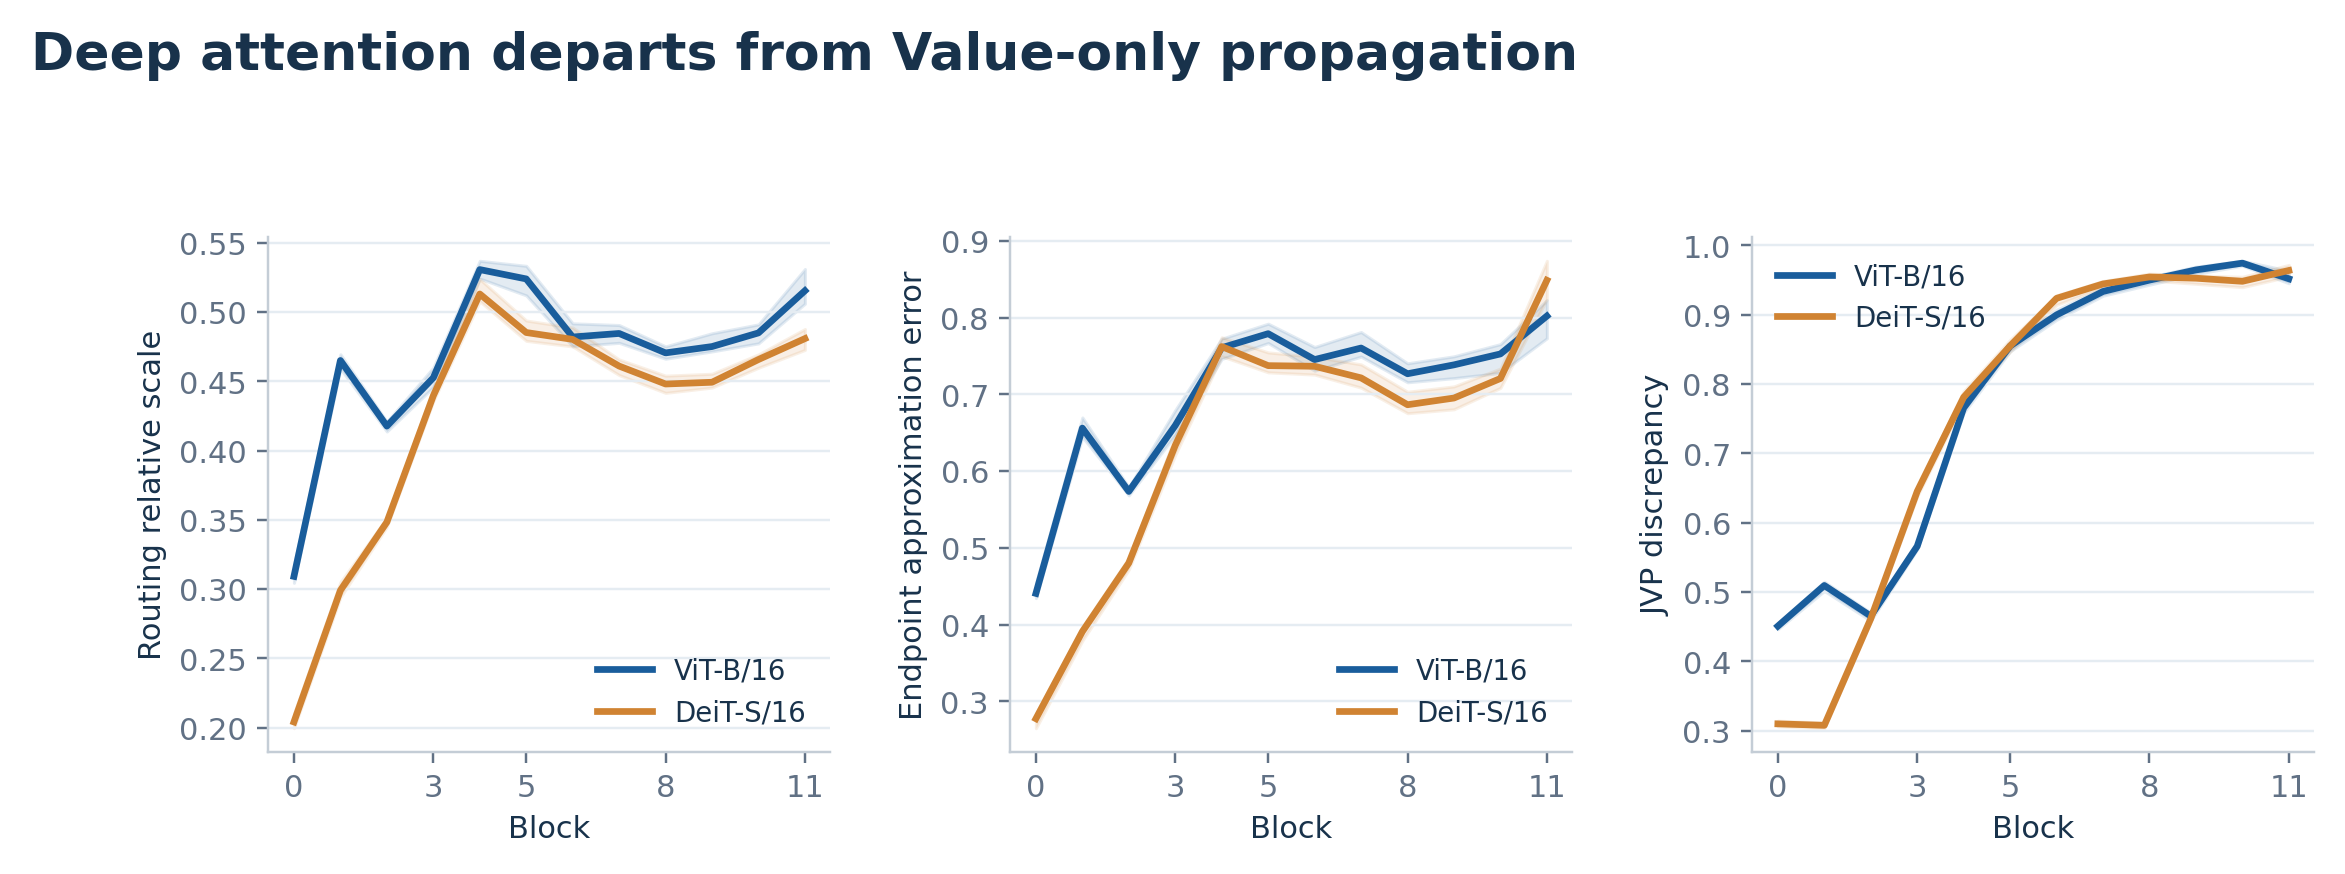
\includegraphics[keepaspectratio,alt={Figure 8}]{../figures/png/fig_16_attention_depth.png}}

\textbf{Figure 8.} 左 panel 为 routing-induced 相对 absolute mass，中
panel 为 Value-only 与完整 attention branch 图的 relative L2 error，右
panel 为冻结方向上的 JVP discrepancy。每个 block 先对图内全部 heads
取中位数，再汇总每 checkpoint 400 图的中位数。阴影为 10,000 次图像
bootstrap 的 95\% 区间。空间图使用 normalized-input 坐标，JVP
使用八个冻结方向。曲线描述固定
checkpoint，层深对比按各模型结果访问前冻结的 family 检验。

\subsection{6.5 Residual identity 与
branch}\label{residual-identity-ux4e0e-branch}

Figure 9 展示两次 residual addition 对同一类别目标的分项。Identity
的输入位置不同，均使用相应 addition 输出处的 cotangent。

\refstepcounter{figure}\label{fig:zh-manuscript-009}
\pandocbounded{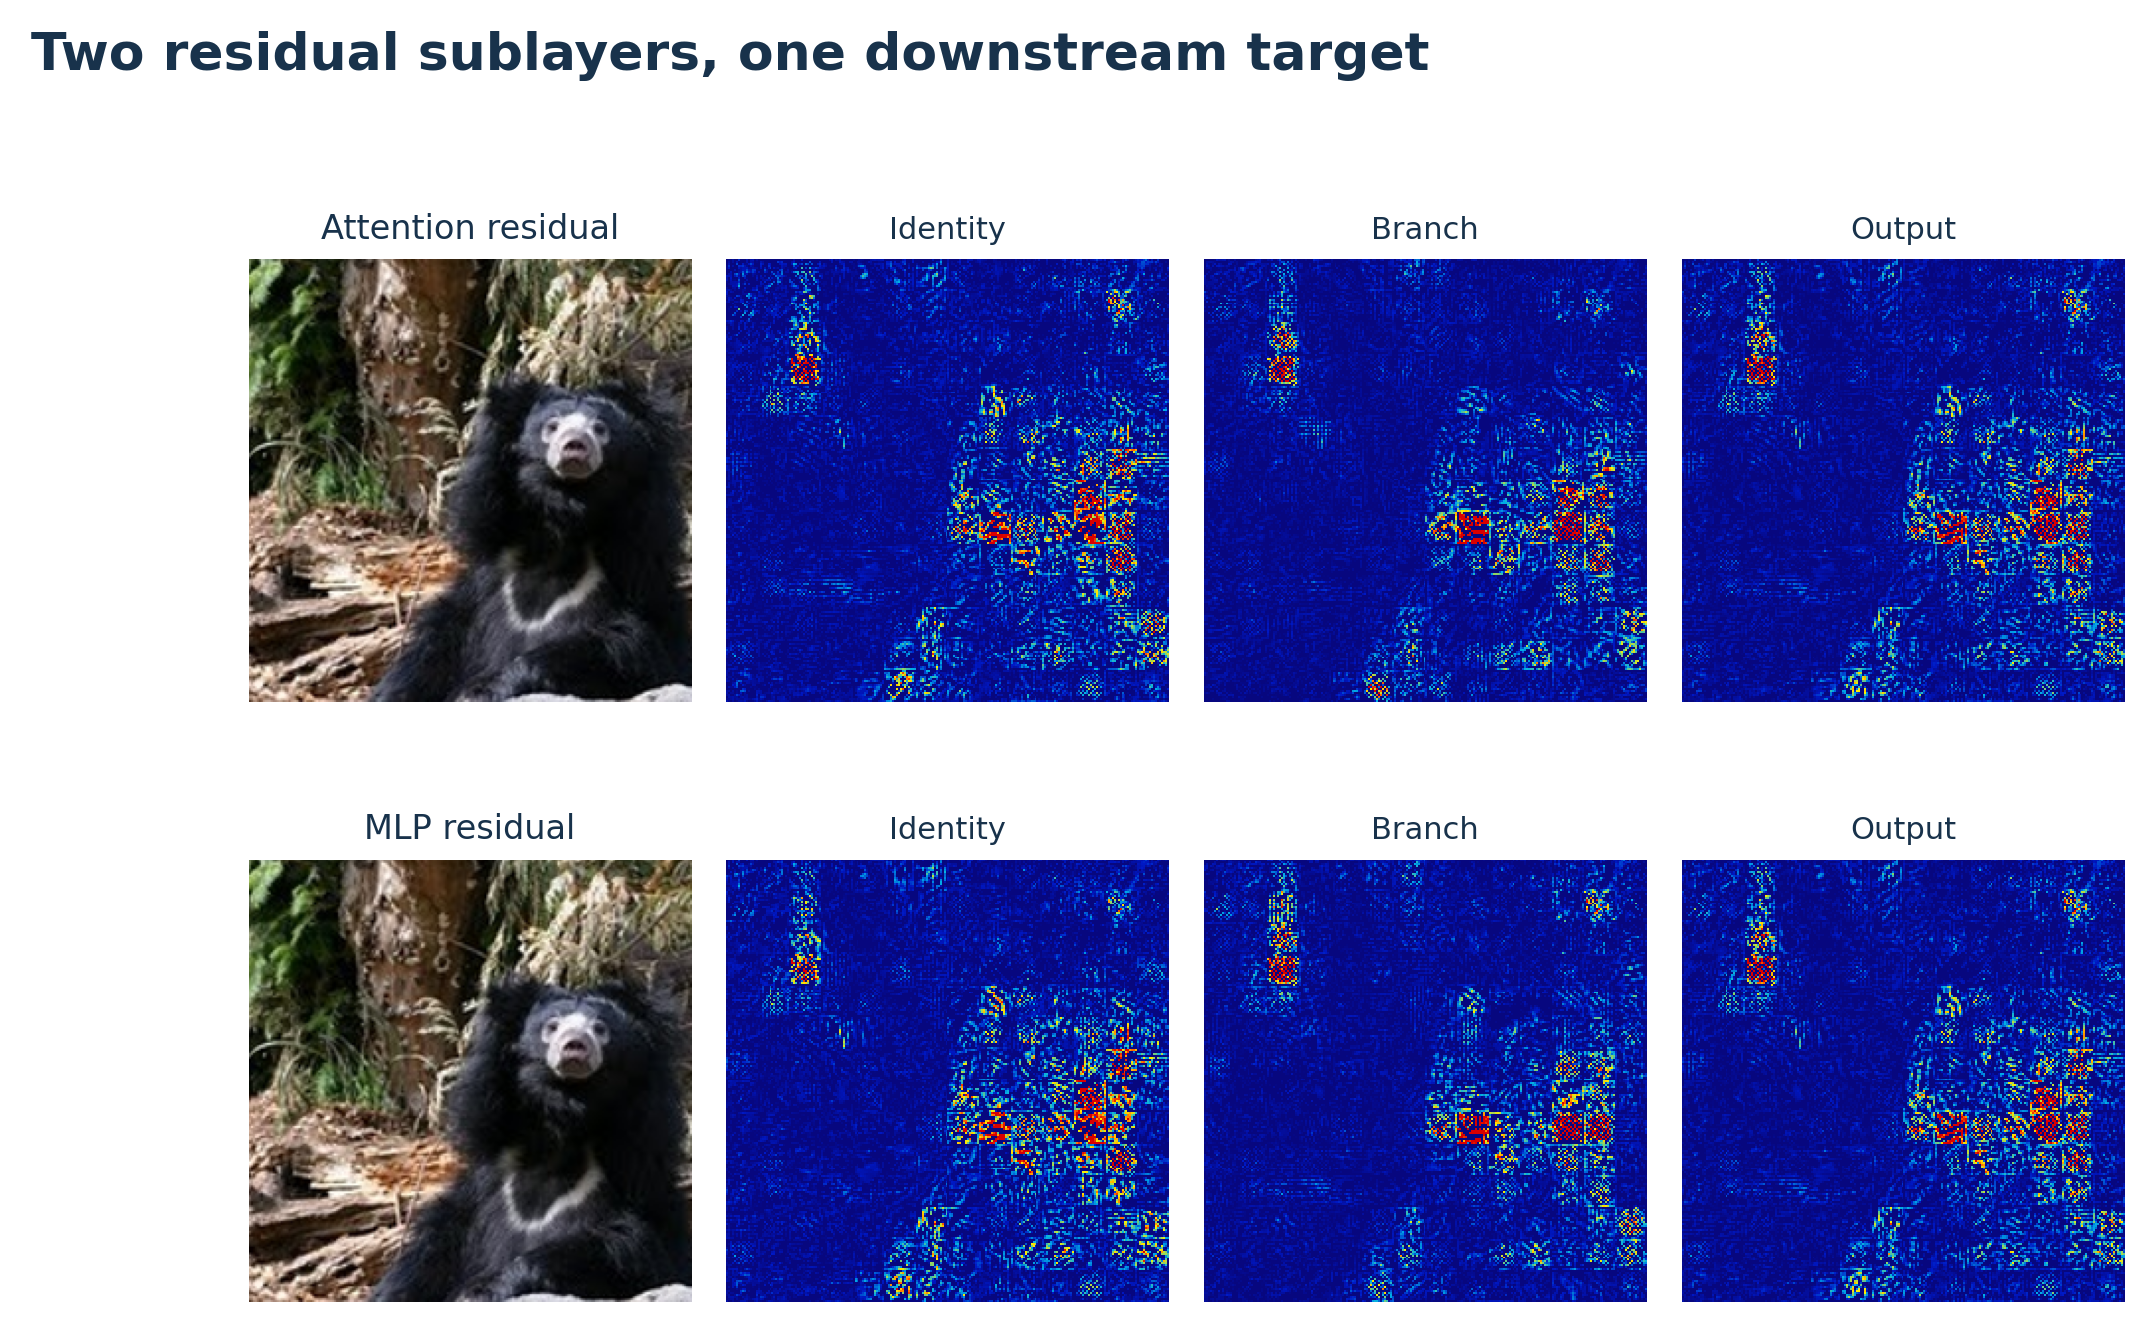
\includegraphics[keepaspectratio,alt={Figure 9}]{../figures/png/fig_17_residual_examples.png}}

\textbf{Figure 9.} 上下两行分别为 DeiT-S/16 block 5 的 attention 与 MLP
residual，同一懒熊输入和 ground-truth
logit。各行从左至右为输入、identity/carry 局部图、branch contribution
和完整目标 Total Endpoint。两种 identity 对应不同 residual 输入；完整
signed 图满足 identity 加 branch 等于 Total Endpoint。正部 panel 按 P99
独立缩放并开方，不能直接相加。单例展示，无统计区间。

Identity relative scale 的 late-minus-early 中位差依次为 attention
-0.124 {[}-0.134, -0.116{]} / -0.045 {[}-0.049, -0.039{]}; MLP 0.180
{[}0.167, 0.189{]} / 0.178 {[}0.166, 0.188{]}。每模型 400 图。

\refstepcounter{figure}\label{fig:zh-manuscript-010}
\pandocbounded{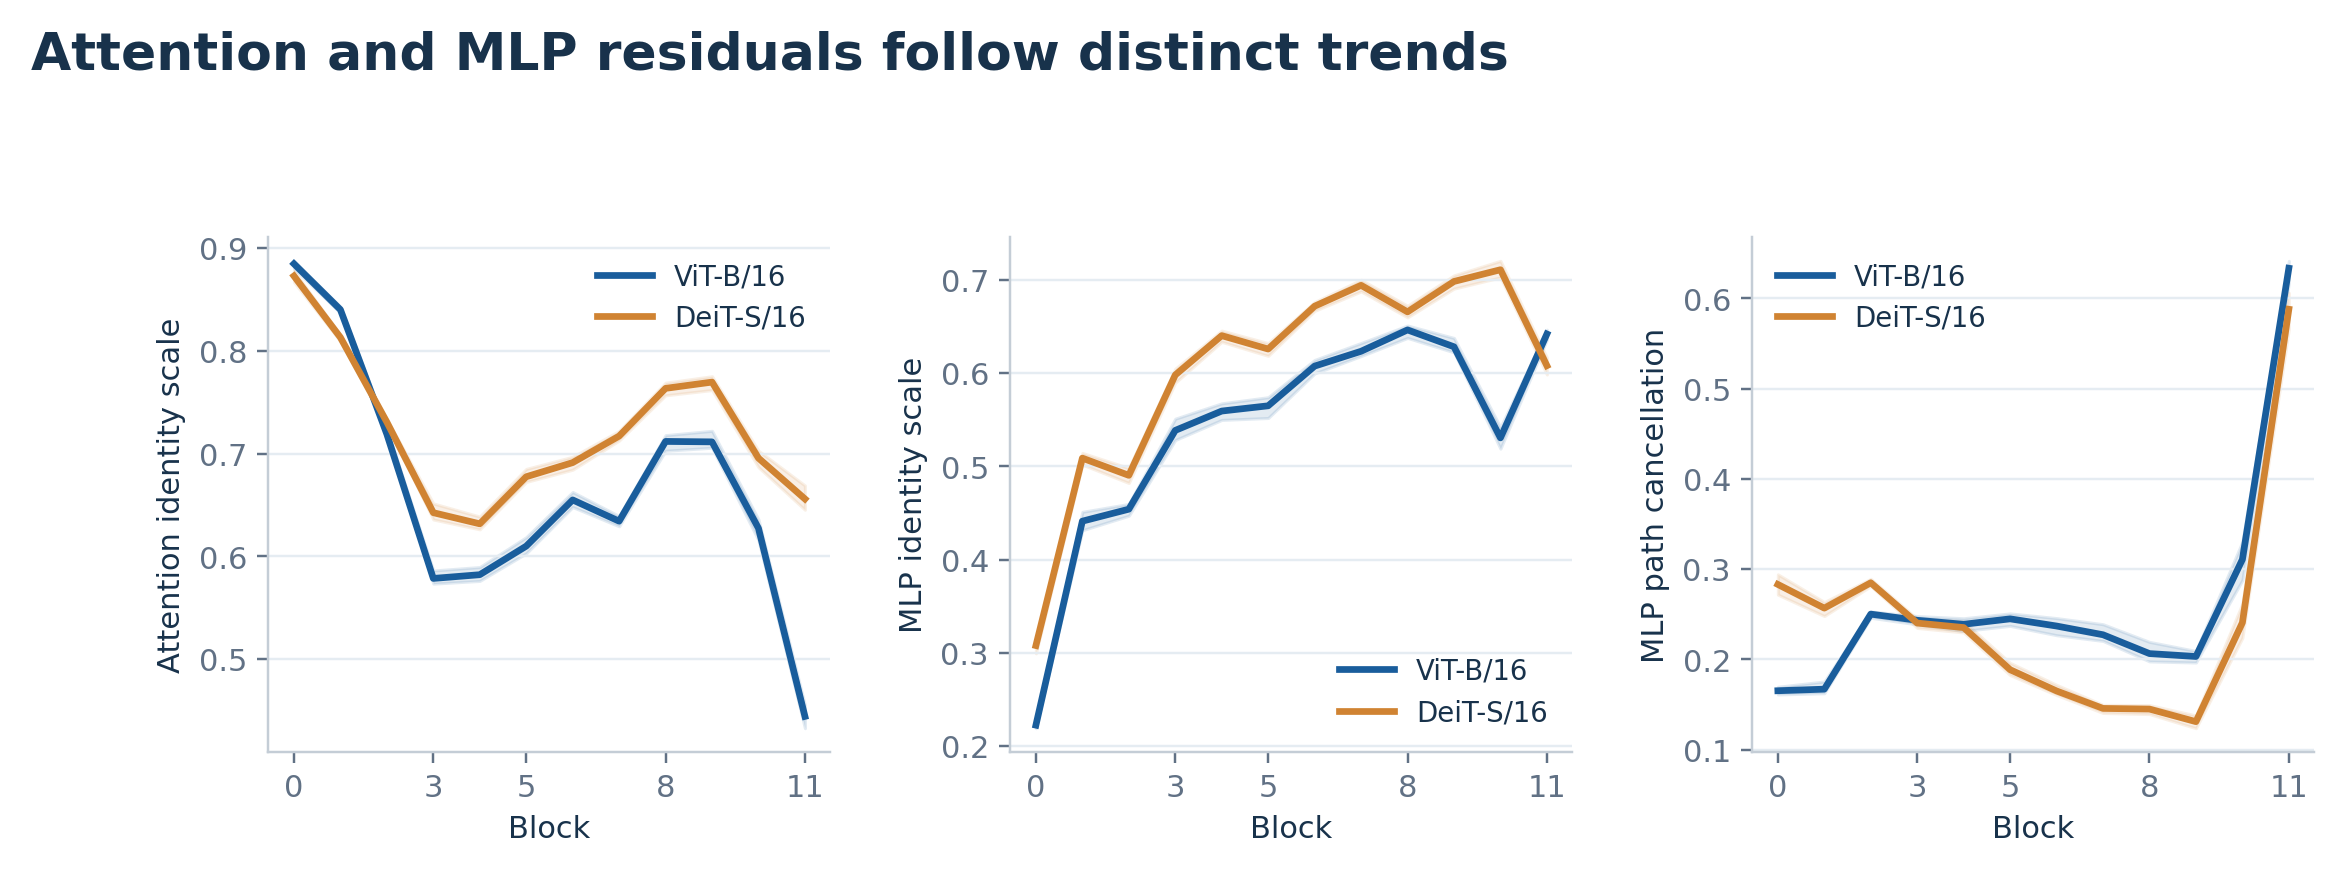
\includegraphics[keepaspectratio,alt={Figure 10}]{../figures/png/fig_18_residual_depth.png}}

\textbf{Figure 10.} 左、中 panel 分别为 attention 和 MLP residual 的
identity relative absolute mass，右 panel 为 MLP identity/branch signed
图的 path cancellation。每图每 block 各有一个对应 residual 值，再取每
checkpoint 400 图的中位数。阴影为 10,000 次图像 bootstrap 的 95\%
区间。全部图使用 normalized-input Endpoint。曲线为固定 checkpoint
描述，层深对比属于结果访问前冻结的分模型 family；后续 output--identity
spatial TV 为单独的事后分析。

独立标为事后的空间 TV 分析比较归一化 output 与 identity patch
mass。Late-minus-early 中位差及 95\% 区间为 vit\_b16 attention 0.052
{[}0.049, 0.055{]}; vit\_b16 mlp -0.019 {[}-0.022, -0.015{]}; deit\_s16
attention 0.028 {[}0.026, 0.030{]}; deit\_s16 mlp -0.046 {[}-0.052,
-0.041{]}。四项检验在单独 Holm family 中通过。总图缺少 identity
身份，edge scalar 缺少空间位置；这项比较同时需要两个索引。

\subsection{6.6 独立队列与四 checkpoint
稳健性检查}\label{ux72ecux7acbux961fux5217ux4e0eux56db-checkpoint-ux7a33ux5065ux6027ux68c0ux67e5}

独立队列在与原始队列和同轮 500 图队列零重叠的 400
张图像上检验四项事前冻结假设。H1 是 32 个 post-block 神经元的 entropy 在
block 11 相对 block 0 的差；H2 是 routing 相对 Q/K-routing 与 V
总质量的比例差；H3 是 MLP residual identity 轨迹减 attention residual
identity 轨迹；H4 是四个代表 block 中，路径图相对 activation × gradient
的 head 排序相关增量。Table 5 报告图像级中位数和 95\% bootstrap 区间。

\refstepcounter{table}\label{tab:zh-manuscript-005}
\textbf{Table 5. 独立队列四 checkpoint 检查；中位数 {[}95\% CI{]}}

{\def\LTcaptype{none} % do not increment counter
\begingroup\scriptsize
\setlength{\tabcolsep}{2pt}
\begin{longtable}[]{@{}
  >{\raggedright\arraybackslash}p{(\linewidth - 10\tabcolsep) * \real{0.1667}}
  >{\raggedright\arraybackslash}p{(\linewidth - 10\tabcolsep) * \real{0.1667}}
  >{\raggedright\arraybackslash}p{(\linewidth - 10\tabcolsep) * \real{0.1667}}
  >{\raggedright\arraybackslash}p{(\linewidth - 10\tabcolsep) * \real{0.1667}}
  >{\raggedright\arraybackslash}p{(\linewidth - 10\tabcolsep) * \real{0.1667}}
  >{\raggedright\arraybackslash}p{(\linewidth - 10\tabcolsep) * \real{0.1667}}@{}}
\toprule\noalign{}
\begin{minipage}[b]{\linewidth}\raggedright
Checkpoint
\end{minipage} & \begin{minipage}[b]{\linewidth}\raggedright
H1
\end{minipage} & \begin{minipage}[b]{\linewidth}\raggedright
H2
\end{minipage} & \begin{minipage}[b]{\linewidth}\raggedright
H3
\end{minipage} & \begin{minipage}[b]{\linewidth}\raggedright
H4
\end{minipage} & \begin{minipage}[b]{\linewidth}\raggedright
Inference
\end{minipage} \\
\midrule\noalign{}
\endhead
\bottomrule\noalign{}
\endlastfoot
vit\_b16 & 0.413 {[}0.405, 0.420{]} & 0.239 {[}0.221, 0.259{]} & 0.851
{[}0.839, 0.865{]} & -0.114 {[}-0.128, -0.091{]} & 400 images; fixed
checkpoint; prospective robustness \\
deit\_s16 & 0.378 {[}0.370, 0.383{]} & 0.322 {[}0.310, 0.329{]} & 0.522
{[}0.495, 0.543{]} & -0.186 {[}-0.229, -0.157{]} & 400 images; fixed
checkpoint; prospective robustness \\
vit\_b16\_in1k & 0.336 {[}0.330, 0.340{]} & 0.241 {[}0.218, 0.255{]} &
0.632 {[}0.620, 0.648{]} & -0.186 {[}-0.205, -0.168{]} & 400 images;
fixed checkpoint; prospective robustness \\
vit\_s16\_augreg & 0.390 {[}0.384, 0.399{]} & 0.276 {[}0.256, 0.296{]} &
0.867 {[}0.840, 0.891{]} & -0.136 {[}-0.171, -0.114{]} & 400 images;
fixed checkpoint; prospective robustness \\
\end{longtable}
\endgroup
}

H4 使用 ground-truth logit 和 normalized-zero reference。对图像
\(j\)、block \(b\) 和 head \(h\)，令 \(z_{jbh}\) 为 \texttt{attn.proj}
输入的 head-channel slice，定义

\begin{equation}\label{eq:zh-manuscript-020}
M_{jbh}=\sum_i|\mathcal L_{jbh,i}|,\qquad
G^{\mathrm{AG}}_{jbh}=|\langle z_{jbh},\nabla_{z_{jbh}}s_j\rangle|,
\end{equation}

\begin{equation}\label{eq:zh-manuscript-021}
Y_{jbh}=|s_j(x)-s_j(x;z_{jbh}\leftarrow z_{jbh}^{\mathrm{normalized\text{-}zero}})|,
\qquad
H4_j=\frac14\sum_{b\in\{0,3,7,11\}}[\rho_h(M_{jbh},Y_{jbh})-\rho_h(G^{\mathrm{AG}}_{jbh},Y_{jbh})].
\end{equation}

\(G^{\mathrm{AG}}\) 先对整个 head
张量作点积再取绝对值，不是逐元素绝对值求和，也不是 attention probability
\(A\)。Spearman 使用平均秩；少于四个有效 heads、非有限或常量向量记为
NA。先在每个 block 的 heads 内计算两项相关之差，再对四个 block
作算术平均；最后在 400 张图像上报告中位数、bootstrap
区间和双侧精确符号检验，并与同 checkpoint 的 H1--H3 一起做四项 Holm
校正。

H1--H3 在四个 checkpoint 中均为正，checkpoint 内 Holm 调整后
\(p<10^{-6}\)。H4 在四个 checkpoint 中均为相反方向，路径图的图内 head
排序相关比 activation × gradient 低 0.114--0.186，Holm 调整后
\(p<10^{-6}\)。空间扩展、routing 与 residual
轨迹在独立图像队列和额外公开 checkpoint 上保持同方向；稳定的路径图 head
排序增量未获支持。新增权重不是独立训练种子。

双索引增加结构分辨率与可审计性；H4 未优于 activation ×
gradient，结构分辨率增加不自动转化为有限干预预测增益。

原 H4 的 path score 先对输入坐标取绝对值再求和，而 activation × gradient
对照先在整个 head tensor 内求和再取绝对值。匹配聚合敏感性将 path score
改为 \(M^{\mathrm{sum}}_{jbh}=|\sum_i\mathcal L_{jbh,i}|\)，其余
target、reference、blocks、effect 与图像级聚合不变。四个 checkpoint
的中位增量仍为负：vit\_b16 −0.124 {[}−0.147, −0.102{]}、deit\_s16 −0.114
{[}−0.157, −0.079{]}、vit\_b16\_in1k −0.226 {[}−0.253,
−0.205{]}、vit\_s16\_augreg −0.171 {[}−0.200,
−0.143{]}。聚合顺序差异因而不能解释原 H4
的阴性方向；该事后分析不替换原注册估计量。

\subsection{6.7
坐标参数化与控制分析}\label{ux5750ux6807ux53c2ux6570ux5316ux4e0eux63a7ux5236ux5206ux6790}

本轮在同一输入点比较 normalized-input Endpoint、raw-pixel gradient 与
RGB 零原点 weighted gradient。完整范围为每模型 100 图固定单元和 400
图结构项，图像是配对统计单位。48 个 phase-summary
组均无缺失，主要方向一致。另报 B11−B0 时，DeiT-S Q 的中位差依次为
−0.004、0.003、0.002，三个区间均跨零，点估计符号改变。完整 96
行中位差、区间及方向见\href{supplement.md\#v6-coordinate}{补充
S17}。主文结论继续限定 normalized-input
Endpoint，对象级方向保持作为补充稳健性结果。

\refstepcounter{table}\label{tab:zh-manuscript-006}
\textbf{Table 5a. 八类核心坐标结果；late-minus-early 中位差（ViT-B /
DeiT-S）。} 三列分别是 normalized-input Endpoint、raw-pixel gradient 和
zero-origin raw-pixel weighted gradient，不统称为三种 Endpoint。

{\def\LTcaptype{none} % do not increment counter
\begingroup\scriptsize
\setlength{\tabcolsep}{2pt}
\begin{longtable}[]{@{}
  >{\raggedright\arraybackslash}p{(\linewidth - 6\tabcolsep) * \real{0.2500}}
  >{\raggedright\arraybackslash}p{(\linewidth - 6\tabcolsep) * \real{0.2500}}
  >{\raggedright\arraybackslash}p{(\linewidth - 6\tabcolsep) * \real{0.2500}}
  >{\raggedright\arraybackslash}p{(\linewidth - 6\tabcolsep) * \real{0.2500}}@{}}
\toprule\noalign{}
\begin{minipage}[b]{\linewidth}\raggedright
Object / metric
\end{minipage} & \begin{minipage}[b]{\linewidth}\raggedright
Normalized-input Endpoint
\end{minipage} & \begin{minipage}[b]{\linewidth}\raggedright
Raw-pixel gradient
\end{minipage} & \begin{minipage}[b]{\linewidth}\raggedright
Zero-origin raw-pixel weighted gradient
\end{minipage} \\
\midrule\noalign{}
\endhead
\bottomrule\noalign{}
\endlastfoot
Unit entropy & 0.220 / 0.225 & 0.240 / 0.245 & 0.217 / 0.221 \\
Unit own-token locality & -0.356 / -0.342 & -0.367 / -0.359 & -0.356 /
-0.356 \\
Unit normalized distance & 0.131 / 0.122 & 0.138 / 0.129 & 0.134 /
0.127 \\
Q entropy & 0.037 / 0.018 & 0.039 / 0.018 & 0.034 / 0.015 \\
K entropy & -0.021 / -0.028 & -0.019 / -0.029 & -0.019 / -0.027 \\
V entropy & -0.010 / -0.013 & -0.009 / -0.016 & -0.010 / -0.015 \\
Attention output--identity TV & 0.052 / 0.028 & 0.054 / 0.028 & 0.053 /
0.027 \\
MLP output--identity TV & -0.019 / -0.046 & -0.017 / -0.044 & -0.018 /
-0.039 \\
\end{longtable}
\endgroup
}

Table 5a 报告轨迹的 phase contrast；DeiT-S Q 的坐标敏感例外来自另一个
B11−B0 estimand，二者不可互换。

训练与随机初始化、GT 与其他类别目标、前向 feature
配对、target-stratum/image
重采样和可视化对比集中于\href{supplement_experiments_v1.md}{补充实验}。随机参数也出现空间扩展，训练状态比较不能识别训练过程因果效应。跨层与全-head
区域替换同样作为补充分析，与原 block-5 本地预先规定分析分开。

\section{7.
规定有限替换任务中的排序能力}\label{ux89c4ux5b9aux6709ux9650ux66ffux6362ux4efbux52a1ux4e2dux7684ux6392ux5e8fux80fdux529b}

\subsection{7.1 规定成分替换与区域诱导的指定-head activation
替换}\label{ux89c4ux5b9aux6210ux5206ux66ffux6362ux4e0eux533aux57dfux8bf1ux5bfcux7684ux6307ux5b9a-head-activation-ux66ffux6362}

成分替换实验的原 12 个 pooled family 作为冻结 provenance
保留；其连续相关、区间和 Holm 调整后 p 值见补充材料。原复合条件中 11/12
达标，但全部成分族的联合判断未获支持。Table 6 优先报告 A 与 V、attention
与 MLP
的事后分层连续结果及类型/层级混合诊断，不用复合计数概括两种不同操作。

\refstepcounter{table}\label{tab:zh-manuscript-007}
\textbf{Table 6. 成分关联的类型与层级诊断；图像级中位数 {[}95\% CI{]}}

{\def\LTcaptype{none} % do not increment counter
\begingroup\scriptsize
\setlength{\tabcolsep}{2pt}
\begin{longtable}[]{@{}
  >{\raggedright\arraybackslash}p{(\linewidth - 14\tabcolsep) * \real{0.1250}}
  >{\raggedright\arraybackslash}p{(\linewidth - 14\tabcolsep) * \real{0.1250}}
  >{\raggedright\arraybackslash}p{(\linewidth - 14\tabcolsep) * \real{0.1250}}
  >{\raggedright\arraybackslash}p{(\linewidth - 14\tabcolsep) * \real{0.1250}}
  >{\raggedright\arraybackslash}p{(\linewidth - 14\tabcolsep) * \real{0.1250}}
  >{\raggedright\arraybackslash}p{(\linewidth - 14\tabcolsep) * \real{0.1250}}
  >{\raggedright\arraybackslash}p{(\linewidth - 14\tabcolsep) * \real{0.1250}}
  >{\raggedright\arraybackslash}p{(\linewidth - 14\tabcolsep) * \real{0.1250}}@{}}
\toprule\noalign{}
\begin{minipage}[b]{\linewidth}\raggedright
Model
\end{minipage} & \begin{minipage}[b]{\linewidth}\raggedright
Reference
\end{minipage} & \begin{minipage}[b]{\linewidth}\raggedright
A-only
\end{minipage} & \begin{minipage}[b]{\linewidth}\raggedright
V-only
\end{minipage} & \begin{minipage}[b]{\linewidth}\raggedright
Attention branch
\end{minipage} & \begin{minipage}[b]{\linewidth}\raggedright
MLP branch
\end{minipage} & \begin{minipage}[b]{\linewidth}\raggedright
Type+block-adjusted A/V
\end{minipage} & \begin{minipage}[b]{\linewidth}\raggedright
Type+block-adjusted residual
\end{minipage} \\
\midrule\noalign{}
\endhead
\bottomrule\noalign{}
\endlastfoot
vit\_b16 & normalized\_zero & 0.049 {[}0.007, 0.091{]} & 0.224 {[}0.192,
0.259{]} & -0.028 {[}-0.056, -0.003{]} & 0.287 {[}0.266, 0.318{]} &
0.030 {[}-0.003, 0.071{]} & -0.128 {[}-0.164, -0.084{]} \\
vit\_b16 & blur\_rgb & 0.073 {[}0.028, 0.112{]} & 0.311 {[}0.266,
0.350{]} & 0.000 {[}-0.021, 0.042{]} & 0.378 {[}0.336, 0.402{]} & -0.018
{[}-0.063, 0.016{]} & 0.042 {[}-0.007, 0.083{]} \\
deit\_s16 & normalized\_zero & 0.091 {[}0.049, 0.119{]} & 0.035
{[}-0.021, 0.087{]} & -0.157 {[}-0.189, -0.119{]} & 0.378 {[}0.346,
0.406{]} & 0.089 {[}0.056, 0.120{]} & -0.091 {[}-0.120, -0.059{]} \\
deit\_s16 & blur\_rgb & 0.101 {[}0.056, 0.133{]} & 0.147 {[}0.112,
0.182{]} & -0.024 {[}-0.070, 0.014{]} & 0.371 {[}0.332, 0.395{]} & 0.095
{[}0.055, 0.128{]} & 0.142 {[}0.096, 0.176{]} \\
\end{longtable}
\endgroup
}

A-only、V-only、attention branch 与 MLP branch 均在每图跨 12 blocks
计算。末两列先对 24 个观测的 predictor 和 effect 分别取秩，再同时控制
operation 与 block；全部结果是事后诊断。A/V 的分层方向和量级依赖模型与
reference；residual pooled 相关主要由 MLP branch 驱动，attention branch
在三项设置中区间覆盖零或为负。类型和层级同时控制后，相关在 ViT-B 两种
reference 下接近零或为负，在 DeiT-S 中随 reference 改变方向。因此旧
pooled 相关只描述混合 family，不能解释为 A、V、attention 或 MLP
类型内部统一的排序能力。完整逐层、仅控制一种因素、Fisher-z head
汇总、A/V concordance、尺度诊断和原 pooled provenance 见补充 S18。

补充同层 head 比较中，Taylor 具有更高 Spearman 与 Capture、更低
Regret（Table 7）。跨层 residual identity 的 Endpoint−Taylor Spearman
差为 0.086--0.421，但 Capture@1 中位差为零，表明增量价值依赖任务和指标。

\refstepcounter{table}\label{tab:zh-manuscript-008}
\textbf{Table 7. 同层 head 排序；图像均值的中位数 {[}95\% CI{]}}

{\def\LTcaptype{none} % do not increment counter
\begingroup\scriptsize
\setlength{\tabcolsep}{2pt}
\begin{longtable}[]{@{}
  >{\raggedright\arraybackslash}p{(\linewidth - 14\tabcolsep) * \real{0.1250}}
  >{\raggedright\arraybackslash}p{(\linewidth - 14\tabcolsep) * \real{0.1250}}
  >{\raggedright\arraybackslash}p{(\linewidth - 14\tabcolsep) * \real{0.1250}}
  >{\raggedright\arraybackslash}p{(\linewidth - 14\tabcolsep) * \real{0.1250}}
  >{\raggedright\arraybackslash}p{(\linewidth - 14\tabcolsep) * \real{0.1250}}
  >{\raggedright\arraybackslash}p{(\linewidth - 14\tabcolsep) * \real{0.1250}}
  >{\raggedright\arraybackslash}p{(\linewidth - 14\tabcolsep) * \real{0.1250}}
  >{\raggedright\arraybackslash}p{(\linewidth - 14\tabcolsep) * \real{0.1250}}@{}}
\toprule\noalign{}
\begin{minipage}[b]{\linewidth}\raggedright
Model
\end{minipage} & \begin{minipage}[b]{\linewidth}\raggedright
Reference
\end{minipage} & \begin{minipage}[b]{\linewidth}\raggedright
Score
\end{minipage} & \begin{minipage}[b]{\linewidth}\raggedright
rho
\end{minipage} & \begin{minipage}[b]{\linewidth}\raggedright
Capture@1
\end{minipage} & \begin{minipage}[b]{\linewidth}\raggedright
Capture@3
\end{minipage} & \begin{minipage}[b]{\linewidth}\raggedright
Regret@1
\end{minipage} & \begin{minipage}[b]{\linewidth}\raggedright
Inference
\end{minipage} \\
\midrule\noalign{}
\endhead
\bottomrule\noalign{}
\endlastfoot
vit\_b16 & normalized\_zero & local\_map & 0.281 {[}0.272, 0.297{]} &
0.517 {[}0.504, 0.535{]} & 0.615 {[}0.609, 0.625{]} & 0.170 {[}0.161,
0.182{]} & 400 images; fixed heads; exploratory \\
vit\_b16 & normalized\_zero & taylor & 0.674 {[}0.666, 0.684{]} & 0.804
{[}0.796, 0.812{]} & 0.857 {[}0.851, 0.862{]} & 0.057 {[}0.052, 0.062{]}
& 400 images; fixed heads; exploratory \\
vit\_b16 & blur\_rgb & local\_map & 0.273 {[}0.259, 0.286{]} & 0.507
{[}0.495, 0.520{]} & 0.618 {[}0.610, 0.626{]} & 0.116 {[}0.112, 0.123{]}
& 400 images; fixed heads; exploratory \\
vit\_b16 & blur\_rgb & taylor & 0.686 {[}0.676, 0.694{]} & 0.820
{[}0.808, 0.835{]} & 0.866 {[}0.860, 0.871{]} & 0.035 {[}0.032, 0.037{]}
& 400 images; fixed heads; exploratory \\
deit\_s16 & normalized\_zero & local\_map & 0.195 {[}0.176, 0.214{]} &
0.561 {[}0.546, 0.574{]} & 0.712 {[}0.705, 0.721{]} & 0.238 {[}0.208,
0.266{]} & 400 images; fixed heads; exploratory \\
deit\_s16 & normalized\_zero & taylor & 0.610 {[}0.600, 0.629{]} & 0.803
{[}0.796, 0.812{]} & 0.889 {[}0.882, 0.895{]} & 0.086 {[}0.079, 0.092{]}
& 400 images; fixed heads; exploratory \\
deit\_s16 & blur\_rgb & local\_map & 0.148 {[}0.133, 0.162{]} & 0.551
{[}0.539, 0.566{]} & 0.710 {[}0.702, 0.716{]} & 0.133 {[}0.117, 0.146{]}
& 400 images; fixed heads; exploratory \\
deit\_s16 & blur\_rgb & taylor & 0.624 {[}0.610, 0.638{]} & 0.843
{[}0.835, 0.852{]} & 0.897 {[}0.893, 0.902{]} & 0.044 {[}0.039, 0.048{]}
& 400 images; fixed heads; exploratory \\
\end{longtable}
\endgroup
}

区域诱导的指定-head activation 替换实验固定 block 5 的三个
heads，所有方法共用 4×4 候选区域及最高 25\% 面积。Figure 11 和 Tables
8--10 给出配对差、绝对 AUC 与归一化 regret。Endpoint−regional Taylor
的配对中位差为 −0.023、−0.024、−0.030、−0.036；四个 family
都未满足相对全部基线的 +0.05
条件。候选集合包络仅取实际评价集合的最优效果，不能视为全部可能区域的全局最优。Clean-only
local map 在该任务中未表现出稳定或实用排序增益；Taylor
较好，但使用了实际位移，信息预算不同，且仍有候选集合包络差距。

\refstepcounter{figure}\label{fig:zh-manuscript-011}
\pandocbounded{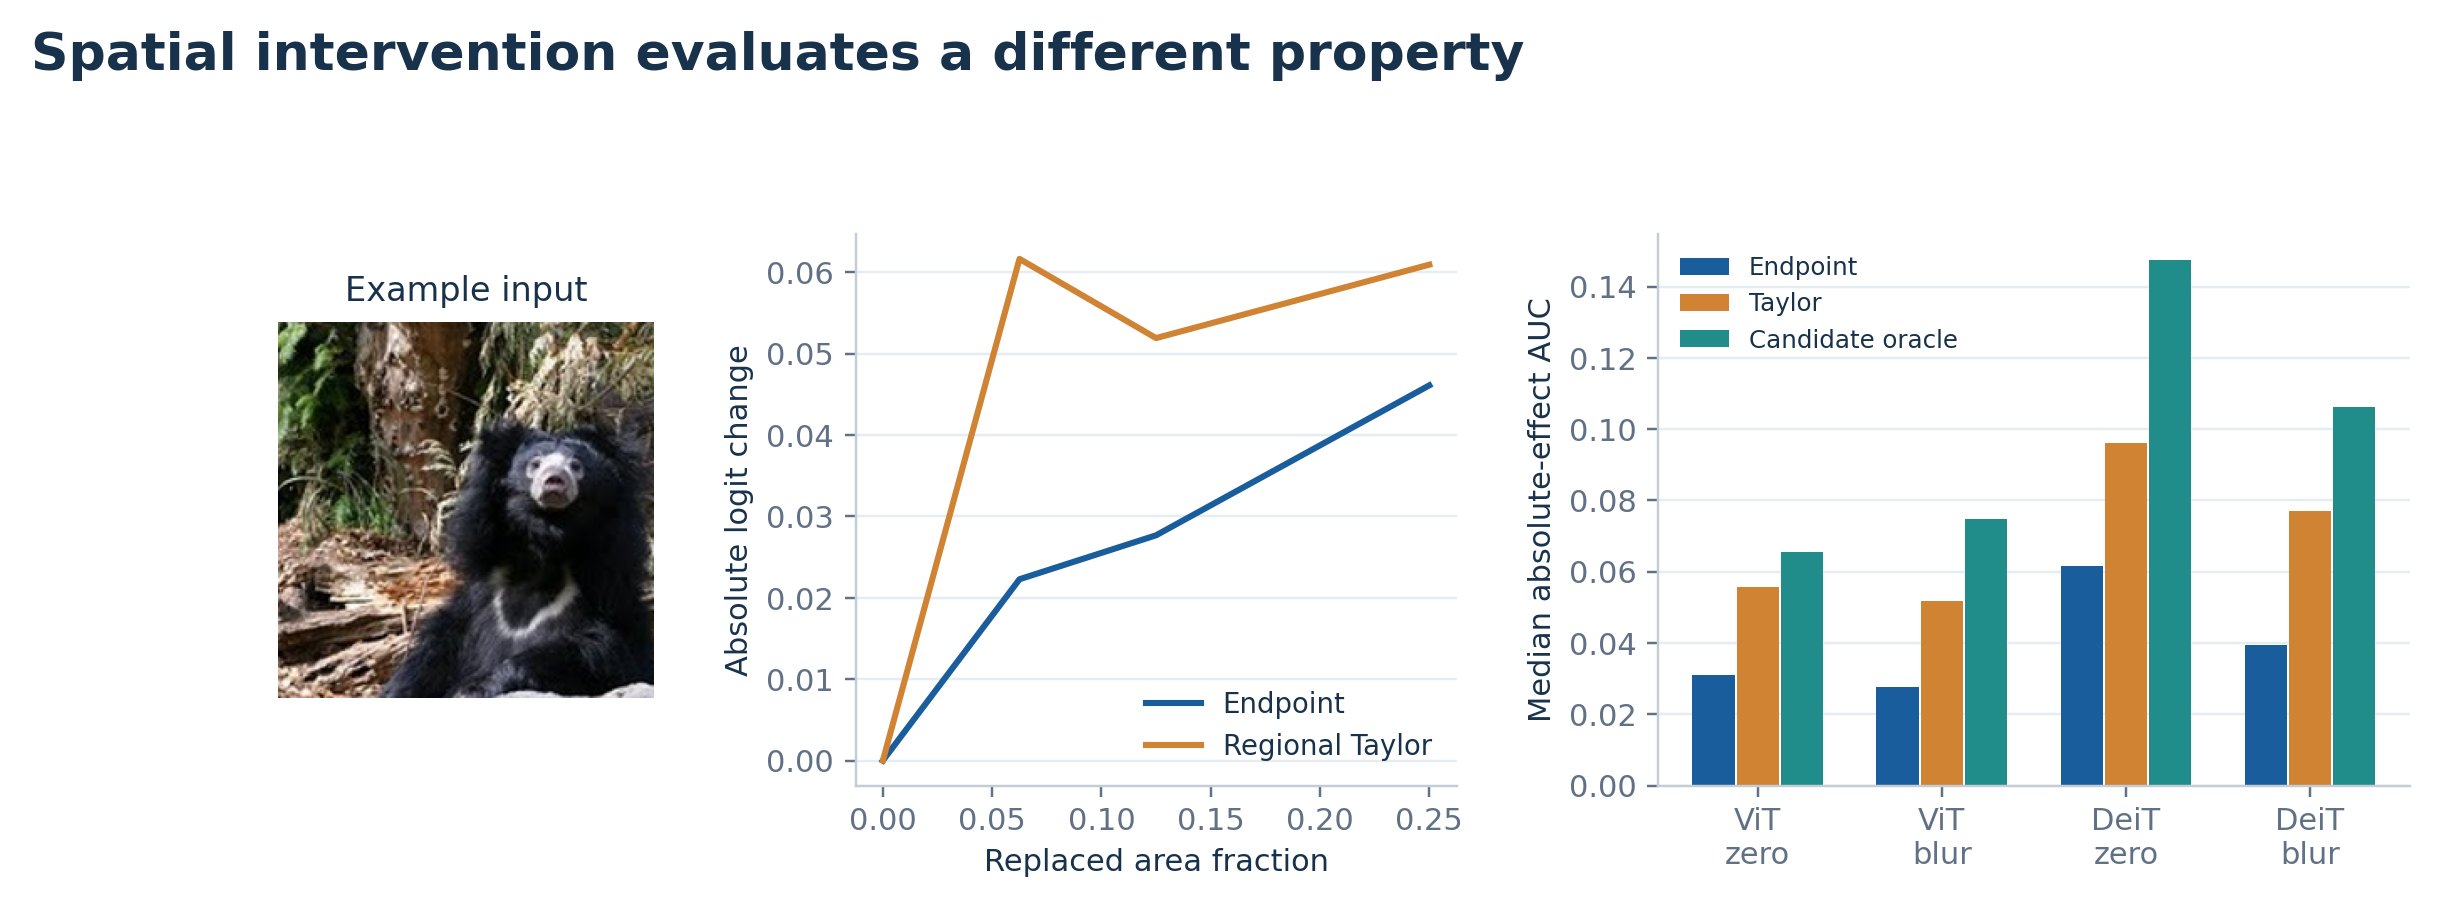
\includegraphics[keepaspectratio,alt={Figure 11}]{../figures/png/fig_21_intervention_boundary.png}}

\textbf{Figure 11.} 左 panel 为 DeiT-S/16 懒熊输入，中 panel 为
normalized-zero reference 下 block 5 三个固定 heads 的 absolute isolated
effect 均值，横轴为替换面积 0、1/16、2/16、4/16。右 panel 为两模型乘两
reference 共四个 family 的图像级 absolute-effect AUC 中位数，每个
n=400，AUC 先在图内按三个 heads 平均。柱图没有误差带，95\% 区间见 Tables
8--10。本图为固定任务的描述性展示；candidate envelope
在每个面积点取已评价候选的最大效果，非单条全局最优策略。

\refstepcounter{table}\label{tab:zh-manuscript-009}
\textbf{Table 8. 局部图 regional AUC 减基线；中位差 {[}95\% CI{]}}

{\def\LTcaptype{none} % do not increment counter
\begingroup\scriptsize
\setlength{\tabcolsep}{2pt}
\begin{longtable}[]{@{}
  >{\raggedright\arraybackslash}p{(\linewidth - 14\tabcolsep) * \real{0.1250}}
  >{\raggedright\arraybackslash}p{(\linewidth - 14\tabcolsep) * \real{0.1250}}
  >{\raggedright\arraybackslash}p{(\linewidth - 14\tabcolsep) * \real{0.1250}}
  >{\raggedright\arraybackslash}p{(\linewidth - 14\tabcolsep) * \real{0.1250}}
  >{\raggedright\arraybackslash}p{(\linewidth - 14\tabcolsep) * \real{0.1250}}
  >{\raggedright\arraybackslash}p{(\linewidth - 14\tabcolsep) * \real{0.1250}}
  >{\raggedright\arraybackslash}p{(\linewidth - 14\tabcolsep) * \real{0.1250}}
  >{\raggedright\arraybackslash}p{(\linewidth - 14\tabcolsep) * \real{0.1250}}@{}}
\toprule\noalign{}
\begin{minipage}[b]{\linewidth}\raggedright
Model
\end{minipage} & \begin{minipage}[b]{\linewidth}\raggedright
Reference
\end{minipage} & \begin{minipage}[b]{\linewidth}\raggedright
vs Total Endpoint regional score
\end{minipage} & \begin{minipage}[b]{\linewidth}\raggedright
vs normalized-coordinate gradient
\end{minipage} & \begin{minipage}[b]{\linewidth}\raggedright
vs reference-aware Taylor
\end{minipage} & \begin{minipage}[b]{\linewidth}\raggedright
vs random
\end{minipage} & \begin{minipage}[b]{\linewidth}\raggedright
Original composite
\end{minipage} & \begin{minipage}[b]{\linewidth}\raggedright
Inference
\end{minipage} \\
\midrule\noalign{}
\endhead
\bottomrule\noalign{}
\endlastfoot
vit\_b16 & normalized\_zero & -0.001 {[}-0.002, -0.0002{]} &
\(-3.1\times10^{-5}\) {[}-0.001, 0.0003{]} & -0.023 {[}-0.026, -0.022{]}
& -0.002 {[}-0.003, -0.001{]} & Unmet & 400 paired images; fixed 3
heads; descriptive intervals \\
vit\_b16 & blur\_rgb & -0.001 {[}-0.002, -0.0002{]} & -0.001 {[}-0.002,
\(3.1\times10^{-5}\){]} & -0.024 {[}-0.027, -0.022{]} & -0.003
{[}-0.005, -0.002{]} & Unmet & 400 paired images; fixed 3 heads;
descriptive intervals \\
deit\_s16 & normalized\_zero & -0.002 {[}-0.003, 0.000{]} & -0.001
{[}-0.002, 0.001{]} & -0.030 {[}-0.034, -0.026{]} & 0.001 {[}-0.001,
0.003{]} & Unmet & 400 paired images; fixed 3 heads; descriptive
intervals \\
deit\_s16 & blur\_rgb & 0.0002 {[}-0.0004, 0.001{]} & -0.0002 {[}-0.001,
0.0005{]} & -0.036 {[}-0.039, -0.031{]} & -0.001 {[}-0.002, 0.001{]} &
Unmet & 400 paired images; fixed 3 heads; descriptive intervals \\
\end{longtable}
\endgroup
}

\refstepcounter{table}\label{tab:zh-manuscript-010}
\textbf{Table 9. 绝对效应 AUC 与 logit；中位数 {[}95\% CI{]}}

{\def\LTcaptype{none} % do not increment counter
\begingroup\scriptsize
\setlength{\tabcolsep}{2pt}
\begin{longtable}[]{@{}
  >{\raggedright\arraybackslash}p{(\linewidth - 14\tabcolsep) * \real{0.1250}}
  >{\raggedright\arraybackslash}p{(\linewidth - 14\tabcolsep) * \real{0.1250}}
  >{\raggedright\arraybackslash}p{(\linewidth - 14\tabcolsep) * \real{0.1250}}
  >{\raggedright\arraybackslash}p{(\linewidth - 14\tabcolsep) * \real{0.1250}}
  >{\raggedright\arraybackslash}p{(\linewidth - 14\tabcolsep) * \real{0.1250}}
  >{\raggedright\arraybackslash}p{(\linewidth - 14\tabcolsep) * \real{0.1250}}
  >{\raggedright\arraybackslash}p{(\linewidth - 14\tabcolsep) * \real{0.1250}}
  >{\raggedright\arraybackslash}p{(\linewidth - 14\tabcolsep) * \real{0.1250}}@{}}
\toprule\noalign{}
\begin{minipage}[b]{\linewidth}\raggedright
Model
\end{minipage} & \begin{minipage}[b]{\linewidth}\raggedright
Reference
\end{minipage} & \begin{minipage}[b]{\linewidth}\raggedright
Local-map regional AUC
\end{minipage} & \begin{minipage}[b]{\linewidth}\raggedright
Taylor AUC
\end{minipage} & \begin{minipage}[b]{\linewidth}\raggedright
Random AUC
\end{minipage} & \begin{minipage}[b]{\linewidth}\raggedright
Candidate-envelope AUC
\end{minipage} & \begin{minipage}[b]{\linewidth}\raggedright
Clean GT logit
\end{minipage} & \begin{minipage}[b]{\linewidth}\raggedright
Inference
\end{minipage} \\
\midrule\noalign{}
\endhead
\bottomrule\noalign{}
\endlastfoot
vit\_b16 & normalized\_zero & 0.031 {[}0.029, 0.032{]} & 0.056 {[}0.053,
0.058{]} & 0.034 {[}0.031, 0.036{]} & 0.065 {[}0.063, 0.070{]} & 8.899
{[}8.842, 8.942{]} & 400 images; fixed 3 heads; descriptive \\
vit\_b16 & blur\_rgb & 0.028 {[}0.026, 0.029{]} & 0.052 {[}0.049,
0.055{]} & 0.031 {[}0.028, 0.033{]} & 0.075 {[}0.068, 0.079{]} & 8.899
{[}8.841, 8.943{]} & 400 images; fixed 3 heads; descriptive \\
deit\_s16 & normalized\_zero & 0.062 {[}0.056, 0.068{]} & 0.096
{[}0.087, 0.103{]} & 0.061 {[}0.057, 0.065{]} & 0.147 {[}0.137, 0.160{]}
& 8.797 {[}8.691, 8.856{]} & 400 images; fixed 3 heads; descriptive \\
deit\_s16 & blur\_rgb & 0.039 {[}0.035, 0.043{]} & 0.077 {[}0.068,
0.082{]} & 0.041 {[}0.038, 0.044{]} & 0.106 {[}0.098, 0.114{]} & 8.797
{[}8.691, 8.856{]} & 400 images; fixed 3 heads; descriptive \\
\end{longtable}
\endgroup
}

\refstepcounter{table}\label{tab:zh-manuscript-011}
\textbf{Table 10. 候选集合遗憾率与 logit 比；中位数 {[}95\% CI{]}}

{\def\LTcaptype{none} % do not increment counter
\begingroup\scriptsize
\setlength{\tabcolsep}{2pt}
\begin{longtable}[]{@{}
  >{\raggedright\arraybackslash}p{(\linewidth - 14\tabcolsep) * \real{0.1250}}
  >{\raggedright\arraybackslash}p{(\linewidth - 14\tabcolsep) * \real{0.1250}}
  >{\raggedright\arraybackslash}p{(\linewidth - 14\tabcolsep) * \real{0.1250}}
  >{\raggedright\arraybackslash}p{(\linewidth - 14\tabcolsep) * \real{0.1250}}
  >{\raggedright\arraybackslash}p{(\linewidth - 14\tabcolsep) * \real{0.1250}}
  >{\raggedright\arraybackslash}p{(\linewidth - 14\tabcolsep) * \real{0.1250}}
  >{\raggedright\arraybackslash}p{(\linewidth - 14\tabcolsep) * \real{0.1250}}
  >{\raggedright\arraybackslash}p{(\linewidth - 14\tabcolsep) * \real{0.1250}}@{}}
\toprule\noalign{}
\begin{minipage}[b]{\linewidth}\raggedright
Model
\end{minipage} & \begin{minipage}[b]{\linewidth}\raggedright
Reference
\end{minipage} & \begin{minipage}[b]{\linewidth}\raggedright
Local-map regional regret
\end{minipage} & \begin{minipage}[b]{\linewidth}\raggedright
Taylor regret
\end{minipage} & \begin{minipage}[b]{\linewidth}\raggedright
Random regret
\end{minipage} & \begin{minipage}[b]{\linewidth}\raggedright
Local-map AUC/abs(logit)
\end{minipage} & \begin{minipage}[b]{\linewidth}\raggedright
Taylor AUC/abs(logit)
\end{minipage} & \begin{minipage}[b]{\linewidth}\raggedright
Inference
\end{minipage} \\
\midrule\noalign{}
\endhead
\bottomrule\noalign{}
\endlastfoot
vit\_b16 & normalized\_zero & 0.530 {[}0.508, 0.555{]} & 0.144 {[}0.132,
0.155{]} & 0.506 {[}0.494, 0.524{]} & 0.004 {[}0.003, 0.004{]} & 0.006
{[}0.006, 0.007{]} & 400 images; fixed 3 heads; descriptive \\
vit\_b16 & blur\_rgb & 0.637 {[}0.607, 0.655{]} & 0.256 {[}0.244,
0.280{]} & 0.593 {[}0.585, 0.600{]} & 0.003 {[}0.003, 0.003{]} & 0.006
{[}0.006, 0.006{]} & 400 images; fixed 3 heads; descriptive \\
deit\_s16 & normalized\_zero & 0.565 {[}0.540, 0.586{]} & 0.335
{[}0.317, 0.357{]} & 0.595 {[}0.583, 0.601{]} & 0.007 {[}0.006, 0.008{]}
& 0.011 {[}0.010, 0.012{]} & 400 images; fixed 3 heads; descriptive \\
deit\_s16 & blur\_rgb & 0.629 {[}0.600, 0.640{]} & 0.271 {[}0.249,
0.295{]} & 0.615 {[}0.607, 0.624{]} & 0.005 {[}0.004, 0.005{]} & 0.009
{[}0.008, 0.010{]} & 400 images; fixed 3 heads; descriptive \\
\end{longtable}
\endgroup
}

修正随机基线后，Endpoint−random 的配对中位差为
−0.002、−0.003、0.001、−0.001；DeiT-S 两个区间跨零。Taylor−random
的四个区间均为正。原 block-5 三-head
结果对应本地预先规定协议；补充跨层全-head 分析覆盖 blocks
2/5/10，在完整输入替换的 11/12 family 与单-head 隔离替换的 12/12 family
显著偏向 Taylor，详见补充实验 S14。

\subsection{7.2 行为标定与 estimand
边界}\label{ux884cux4e3aux6807ux5b9aux4e0e-estimand-ux8fb9ux754c}

跨 reference 分析补充了这一结果的含义。Endpoint 使用观测输入处的 clean
map，而 Taylor 显式使用替换位移。对 163,200 个成分配对，Taylor magnitude
与 absolute effect 在原 atol=1e-12、rtol=0 标准下均发生变化；分布及 head
排名一致性见补充表。Reference
会改变干预相关排序，局部输入图与位移估计器因而适用于不同问题。

\section{8. 讨论与结论}\label{ux8ba8ux8bbaux4e0eux7ed3ux8bba}

\subsection{8.1 讨论}\label{ux8ba8ux8bba}

双索引图使指定 use
或微分分组的空间分布可直接比较。总图可描述整体空间扩展，component scalar
可描述尺度，Q/K/V entropy 与 residual output--identity TV
则需要路径标签和输入位置。全局切面包含 bypass，branch partition 只重构
attention contribution。该区分使闭合目标与后续解释保持一致。

架构图认证把这一合同落实到实际 target--cut
配对，而不从单点数值闭合反推图结构。三类 registry
则分别约束标量读出、局部微分分解和有限替换变量，避免用同一个``注册对象''名称混合不同数学对象。

经验结论以固定 checkpoint 和抽样目标上的 normalized-input Endpoint
为对象。单元扩展、K/V 熵与 residual TV
的主要方向对三种已测输入表示保持；DeiT-S Q 的 B11−B0
则存在坐标和区间敏感性。等价隐藏坐标变换也可改变分项而保持总
Endpoint，因而这些图描述指定实现的局部微分结构。

H4 在四个 checkpoint 上均低于 activation ×
gradient。双索引图增加结构分辨率与可审计性，没有自动提高有限干预预测。Taylor
直接使用 replacement displacement，在规定区域任务中更适合排序。旧 pooled
成分关联为正，但 v7 分层显示 A/V 与 attention/MLP 不是同质
family；类型和层级控制后的相关具有模型与 reference 依赖。原 all-family
判断仍未获支持，行为结果保持广泛但非普遍。

图像区间条件于固定 targets 和
checkpoint，不代表神经元或架构总体。独立图像队列仍由同团队和代码分析；公开
checkpoint 差异不识别训练过程的因果效应。Random
参数也出现空间扩展。显示正部用于阅读空间结构，数值推断使用完整
signed/absolute 数组。ViT-B Path IG 的历史校准失败保留，未进行跨模型
Endpoint--Path 推断。

\subsection{8.2 方法局限}\label{ux65b9ux6cd5ux5c40ux9650}

当前点一阶 Jacobian
描述局部响应，不刻画大位移下的非线性交互。分项依赖指定计算图、内部坐标和切面，不具一般实现不变性。极小梯度、饱和与归一化会改变空间形状指标，归一化后的
TV 不是功能重要性。实证范围限于 ImageNet、patch-16
ViT、固定标量目标和规定的 replacement
contracts；向量目标只能经预先声明的标量函数或逐坐标分析扩展，本文未验证序列模型和其他架构。不同
checkpoint
的训练、规模与数据因素没有被当前设计分离，因而模型异质性的原因未识别。

\subsection{8.3 结论}\label{ux7ed3ux8bba}

精确当前点导数传播下，标量 NNS learning image 等于 Gradient ×
Input。本文的技术贡献是目标条件化双索引表示、分支与全局闭合合同，以及针对实际
ViT 切面和具体 use 错误的结构与数值审计。固定抽样目标的 normalized-input
Endpoint 呈现与 block index
相关的空间轨迹；该扩展方向在总质量分层与截尾分析中保持，但熵数值具有质量依赖。Q
分项对模型和输入坐标更敏感，路径图在原聚合与匹配聚合下均未优于
activation × gradient 的 head
有限替换排序。规定替换的关联广泛但非普遍，不支持统一合并结论。结构分辨率和可审计性增加不自动转化为有限干预预测增益。

\section{参考文献与补充材料}\label{ux53c2ux8003ux6587ux732eux4e0eux8865ux5145ux6750ux6599}

参考文献列于文末；补充材料随稿提交。

\section*{参考文献}\label{bibliography}
\addcontentsline{toc}{section}{参考文献}

\protect\phantomsection\label{refs}
\begin{CSLReferences}{1}{1}
\bibitem[\citeproctext]{ref-abnar2020attention}
Abnar, Samira, and Willem Zuidema. 2020. {``Quantifying Attention Flow
in Transformers.''} \emph{ACL}.

\bibitem[\citeproctext]{ref-achtibat2024attnlrp}
Achtibat, Reduan, Sayed Mohammad Vakilzadeh Hatefi, Maximilian Dreyer,
et al. 2024. {``AttnLRP: Attention-Aware Layer-Wise Relevance
Propagation for Transformers.''} \emph{ICML}.

\bibitem[\citeproctext]{ref-buratti2026gradskip}
Buratti, Christopher, Michele Marchetti, Federico Parlapiano, Daniele
Traini, Domenico Ursino, and Luca Virgili. 2026. \emph{Gradient-Skipping
Relevance Propagation for Efficient Explainability of Vision
Transformers}. \url{https://doi.org/10.48550/arXiv.2607.10365}.

\bibitem[\citeproctext]{ref-chefer2021transformer}
Chefer, Hila, Shir Gur, and Lior Wolf. 2021. {``Transformer
Interpretability Beyond Attention Visualization.''} \emph{CVPR}.

\bibitem[\citeproctext]{ref-chen2026unpack}
Chen, Po-Kai, Aske Plaat, and Niki van Stein. 2026. \emph{Every
Component Is a Lookup: Token Attribution and Composition from a Single
Decomposition}. \url{https://doi.org/10.48550/arXiv.2605.23393}.

\bibitem[\citeproctext]{ref-dhamdhere2018conductance}
Dhamdhere, Kedar, Mukund Sundararajan, and Qiqi Yan. 2018. {``How
Important Is a Neuron?''} \emph{arXiv Preprint arXiv:1805.12233}.

\bibitem[\citeproctext]{ref-dosovitskiy2021vit}
{Dosovitskiy, Alexey, Lucas Beyer, Alexander Kolesnikov, et al.} 2021.
{``An Image Is Worth 16x16 Words: Transformers for Image Recognition at
Scale.''} \emph{ICLR}.

\bibitem[\citeproctext]{ref-dou2023nns}
Dou, Hongtao, Furao Shen, Jian Zhao, and Xiyu Mu. 2023. {``Understanding
Neural Network Through Neuron Level Visualization.''} \emph{Neural
Networks} 168: 484--95.
\url{https://doi.org/10.1016/j.neunet.2023.09.030}.

\bibitem[\citeproctext]{ref-ferrando2022alti}
Ferrando, Javier, Gerard I. Gallego, and Marta R. Costa-jussa. 2022.
{``Measuring the Mixing of Contextual Information in the Transformer.''}
\emph{EMNLP}.

\bibitem[\citeproctext]{ref-izadi2026caap}
Izadi, Amirhossein, Mohammad Banayeeanzade, Amin Mirrokni, et al. 2026.
\emph{Causal Attribution via Activation Patching}.
\url{https://doi.org/10.48550/arXiv.2603.13652}.

\bibitem[\citeproctext]{ref-kramar2024atp}
Kramar, Janos, Tom Lieberum, Rohin Shah, and Neel Nanda. 2024.
\emph{AtP*: An Efficient and Scalable Method for Localizing LLM
Behaviour to Components}. \url{https://arxiv.org/abs/2403.00745}.

\bibitem[\citeproctext]{ref-mehri2025libragrad}
Mehri, Faraz, Mahdieh Soleymani Baghshah, and Mohammad Taher Pilehvar.
2025. {``LibraGrad: Balancing Gradient Flow for Universally Better
Vision Transformer Attributions.''} \emph{CVPR}.

\bibitem[\citeproctext]{ref-modarressi2023decompx}
Modarressi, Ali, Mohsen Fayyaz, Ehsan Aghazadeh, Yadollah Yaghoobzadeh,
and Mohammad Taher Pilehvar. 2023. {``DecompX: Explaining Transformers
Decisions by Propagating Token Decomposition.''} \emph{ACL}.

\bibitem[\citeproctext]{ref-modarressi2022globenc}
Modarressi, Ali, Mohsen Fayyaz, Yadollah Yaghoobzadeh, and Mohammad
Taher Pilehvar. 2022. {``GlobEnc: Quantifying Global Token Attribution
by Incorporating the Whole Encoder Layer in Transformers.''}
\emph{NAACL-HLT}.

\bibitem[\citeproctext]{ref-nishankar2026hilrp}
Nishankar, S., P. Sanjeewani, A. Perera, and S. Thuseethan. 2026.
\emph{HiLRP: Toward One Trustworthy Explanation for Vision Transformer:
Conservation-Valid Attribution via Attention Primitives}.
\url{https://doi.org/10.48550/arXiv.2609.01282}.

\bibitem[\citeproctext]{ref-selvaraju2017gradcam}
Selvaraju, Ramprasaath R., Michael Cogswell, Abhishek Das, Ramakrishna
Vedantam, Devi Parikh, and Dhruv Batra. 2017. {``Grad-CAM: Visual
Explanations from Deep Networks via Gradient-Based Localization.''}
\emph{ICCV}.

\bibitem[\citeproctext]{ref-shrikumar2017deeplift}
Shrikumar, Avanti, Peyton Greenside, and Anshul Kundaje. 2017.
{``Learning Important Features Through Propagating Activation
Differences.''} \emph{ICML}.

\bibitem[\citeproctext]{ref-srinivas2019fullgrad}
Srinivas, Suraj, and Francois Fleuret. 2019. {``Full-Gradient
Representation for Neural Network Visualization.''} \emph{NeurIPS}.

\bibitem[\citeproctext]{ref-sundararajan2017ig}
Sundararajan, Mukund, Ankur Taly, and Qiqi Yan. 2017. {``Axiomatic
Attribution for Deep Networks.''} \emph{ICML}.

\bibitem[\citeproctext]{ref-syed2024eap}
Syed, Aaquib, Can Rager, and Arthur Conmy. 2024. {``Attribution Patching
Outperforms Automated Circuit Discovery.''} \emph{BlackboxNLP}.
\url{https://doi.org/10.18653/v1/2024.blackboxnlp-1.25}.

\bibitem[\citeproctext]{ref-wrobel2026dave}
Wrobel, Aleksandra, Siddhartha Gairola, Jacek Tabor, Bernt Schiele,
Bartosz Zielinski, and Dawid Rymarczyk. 2026. \emph{DAVE:
Distribution-Aware Attribution via ViT Gradient Decomposition}.
\url{https://doi.org/10.48550/arXiv.2602.06613}.

\bibitem[\citeproctext]{ref-zhang2023patching}
Zhang, Fred, and Neel Nanda. 2023. \emph{Towards Best Practices of
Activation Patching in Language Models: Metrics and Methods}.
\url{https://arxiv.org/abs/2309.16042}.

\bibitem[\citeproctext]{ref-zukowska2026vicd}
Zukowska, Natalia, Wolfgang Stammer, Bernt Schiele, and Jonas Fischer.
2026. \emph{Seeing Through Circuits: Faithful Mechanistic
Interpretability for Vision Transformers}.
\url{https://doi.org/10.48550/arXiv.2604.14477}.

\end{CSLReferences}


\begingroup\color{white}\fontsize{0.1pt}{0.1pt}\selectfont \ref{fig:zh-manuscript-001}; \ref{fig:zh-manuscript-011}; \ref{tab:zh-manuscript-001}; \ref{tab:zh-manuscript-011}; \ref{eq:zh-manuscript-001}; \ref{eq:zh-manuscript-021}\endgroup
\end{document}
